This section consist of a case study where a model is specified and estimated based on the method proposed in Section \ref{seq:mdp}.
As discussed in section XXX %TODO 
it can be very computationally demanding to estimate a model using NFXP. We have therefore chosen to restrict this case study to the special case when there is no uncertainty in the transition of the state variables in $x_k$ and when the scale of the random state variables $\epsilon$ is the same in all $x_k$ so that $\mu(x_k)=\mu=1$. As discussed in \ref{sec:estSampling}, this special case can be estimated using sampling of alternative sequences of actions. We further use the estimates to generate statistics of, e.g., the departure time of trips. 


% Description of what type of behaviour we set out to model in our case study.

People can have fixed or flexible working hours. People with fixed working hours must arrive at work when the workday start and leave when the workday ends. %Specify how this is done: +-10minutes is ok.
People with flexible working hours can choose to arrive between $6\unit{a.m.}$ and $10\unit{a.m.}$, but the length of a working day is still fixed. The individual specifications on working hour type, working length, start and end hours must be provided from elsewhere. Children can be dropped off between $6:30\unit{a.m.}$ and $12:00\unit{a.m.}$. Pick up trips must be completed between $12\unit{a.m.}$ and $6:30\unit{p.m.}$

\subsection{Model specification}
In this case study we will describe the daily planning of travel and activities of individuals with fairly regular working schedules on working days. We have assumed that 



\newcommand{\p}[1]{p_{\text{#1}}}
\newcommand{\m}[1]{m_{\text{#1}}}
\newcommand{\amemm}[1]{\amem_\text{#1}}


An individual has a set of mandatory activities which has to be performed during a day and for which the location is fixed. For all individuals $\p{work}$ is in this set, and depending on if they are observed to drop of or pick up children during the day those activities may also be mandatory.  
\subsubsection{Actions}
Remember that an action consisted of the choice of a location, activity and mode. We have used the so called EMME zonal system of the region of Stockholm, which is standard to use in models in the area and for which official statics are available. The Stockholm region consist of 1240 such zones, so $N_L = 1240$. The modes modelled are car, public transport, bike and walk. Activities are divided into home, work, child (pick up or drop off), social, recreational, grocery shopping and other.

\begin{equation} 
a_k = \begin{pmatrix}
\act{d} \\
\act{m} \\
\act{p}    
\end{pmatrix}
\subset
\begin{Bmatrix*}[l]
\{1,2,\dots, 1240\}, \\
\{m_{\text{stay}},\m{car},\m{pt},\m{walk},\m{bike}\}, \\
\{ p_{\text{travel}},p_{\text{end}},\p{home},\p{work},\p{child},\p{rec.},\p{social},\p{shop},\p{other}\} 
\end{Bmatrix*}
\end{equation}
\subsubsection{States}
We let a day start at $5\unit{am}$ and end at $11\unit{pm}$, and let $t$ define the number of $10\units{minute}$ intervals since $5\unit{am}$ so that $T=108$.
We will for the case study let the marginal utility of activity participation be constant, so $N_\atime=\max{N_{\atime,p}}=0$. The mode history will be dependent on whether the previous car is a car or not, which will influence the availability of a car. The mode history can thus be described by three values: $m_{\text{stay}},\m{car}$ and $\m{pt}$. The activity history will be described by whether any of the mandatory activities have been performed, where $\amemm{no}$ means that no mandatory activity has been performed and $\amemm{activity}$ means that 'activity' was the last previous mandatory activity to be performed. 
\begin{equation}
\s{k} = \begin{pmatrix}
t \\
l \\
p \\
\atime\\
m \\
\amem \\
\epsilon
\end{pmatrix}
\subset
\begin{Bmatrix*}[l]
[0,108] \\
\{1,2,\dots, 1240\} \\
\{ p_{\text{travel}},p_{\text{end}},\p{home},\p{work},\p{child},\p{rec.},\p{social},\p{shop},\p{other}\}  \\
\{0\} \\
\{m_{\text{stay}},\m{car},\m{pt} \}\\
\{\amemm{no},\amemm{drop off}, \amemm{work},\amemm{pickup}\}\\
\rr^{N_C}
\end{Bmatrix*}
\end{equation}

\subsubsection{Conditional choice-set}
The choice set $C(s_k)$ has been specified in \eqref{eq:choiceset} up to the opening hours of activities $t^{\text{open}}({l,p})$


\subsubsection{State transitions}

\subsubsection{One-stage utility functions}
\newcommand{\cost}{\text{cost}}
\newcommand{\car}{\text{car}}
\newcommand{\pt}{\text{PT}}
\newcommand{\walk}{\text{walk}}
\newcommand{\bike}{\text{bike}}
\newcommand{\dummy}[1]{\delta_{#1}}
\newcommand{\hi}{\text{h.i}}
\newcommand{\wait}{\text{wait}}
\newcommand{\geqfive}{\text{s.z.,walk}}
\newcommand{\mc}{\theta}
\newcommand{\ac}{C}
\newcommand{\acp}{\theta}
\newcommand{\dura}[1]{\Delta t_#1}
\newcommand{\TT}{TT}
\newcommand{\ustay}{\avgu_\text{stay}}
\newcommand{\stay}{\text{stay}}

The one-stage utility of a state-action pair was in \eqref{eq:mdponestage} dividable into one part for the (dis)utility of travelling and one part for the activity of utility participation. Below follows the specification of these two utility functions used in the case study, starting with the utility of travelling.
\paragraph{Utility of travelling}
The utility of travelling is given by:
\begin{equation}
u_{trav}(t,l,m,\act{d},\act{m}) = \mc_{\act{m}} + \theta_{tt,\act{m}} \cdot \TT_{\act{m}}(t,l,\act{d}) + \theta_{\cost} \cdot C_{\act{m}}(t,l,\act{d}) +\theta_{\geqfive} \dummy{\geqfive}
\end{equation}
where $\mc_{\act{m}}$ are mode specific constants; $\theta_{tt,\act{m}}$ are mode specific (dis)utilities for travel time  $\TT_{\act{m}}(t,l,\act{d})$ and $C_{\act{m}}(t,l,\act{d})$ denote the travel time and cost with mode $\act{m}$ at time $t$ for a trip from origin $l$ to destination $\act{d}$; and $\dummy{\geqfive}$ is a dummy indicating if the trip is done within the same zone with walk. Observe that the mode state $m$ does not influence the one-stage utility in the case-study specification.

\paragraph{Utility of activity participation}
From \eqref{eq:mdponestage}, the one-stage utility when participating in an activity is given is dependent on the state variables for location $l$, time $t$, purpose $p$, activity history $\atime$, and the number of time-steps an activity has been performed $\amem$. In the case study, the activity of utility participation will be given by:
\begin{equation}
	\avgu_{act}(l,t,p,\atime,\amem) = \ustay(t,\act{p},\dura{p}) + \begin{cases} 
	\ac_p(t) + u_{p,\text{size}}(l) &\cif p = p_{\text{travel}} \\
	0 & \celse
	\end{cases}
\end{equation}
where $\ustay(t,\act{p},\dura{p})$ is the potentially time-of-day dependent utility obtained when staying and continuing with the activity for a duration of $\dura{p}$; $\ac_p(t)$ is a time-of-day dependent utility for starting an activity; and $u_{p,\text{size}}(l)$ is a location dependent utility obtained when starting an activity in a specific location, modelling the availability of services. In order to keep down the number of parameters in the case study, the constant utility $\ac_p(t)$ is only time dependent for the work activity and the duration utility $\ustay(t,\act{p},\dura{p})$ is only time dependent for the home activity. Time-of-day varying parameters are specified on discrete time steps $T_k$ with values $\theta_{\stay,p,T_k}$ and $\acp_{C,p,T_k}$. The time-of-day dependent utility of starting an activity is given by linear interpolation between the closest defined parameters:
\begin{equation*}
\ac_p(t) = \frac{\acp_{C,p,T_k}\cdot (T_{k+1}-t)+\acp_{C,p,T_{k+1}}\cdot (t-T_k)}{T_{k+1}-T_{k}}
\end{equation*}
where $t\in(T_k,T_{k+1})$. For the duration utility we specify the \emph{marginal} utility of activity participation at time $t$ as given by linearly interpolation between the closest parameters, so:
\begin{equation*}
u_\text{stay,marg}(t,\act{p}) = \frac{\theta_{\stay,p,T_k}\cdot(T_{k+1}-T_k)+\theta_{\stay,p,T_{k+1}}\cdot(t-T_k) }{T_{k+1}-T_{k}}.
\end{equation*}
The stay-utility of an activity episode of duration $\dura{p}$, when $T_k\leq t$ and $t+\dura{p}\leq T_{k+1}$, then becomes:
\begin{equation} \label{eq:uacttime}
\begin{aligned}
\ustay(t,\act{p}) &= \int_t^{t+\dura{p}} u_\text{stay,marg}(\tau,p) % \frac{\theta_{p,T_k}(T_{k+1}-\tau)+\theta_{p,T_{k+1}}(\tau-T_k) }{T_{k+1}-T_{k}}
\ud{\tau} = \alpha_{T_k}\theta_{\stay,p,T_k} + \alpha_{T_{k+1}}\theta_{\stay,p,T_{k+1}}% \\
%&= \frac{\theta_{p,T_k}T_{k+1}-\theta_{p,T_{k+1}}T_k + (\theta_{p,T_{k+1}} - \theta_{p,T_{k}}) (2t\dura{p} + \dura{p}^2)}{T_{k+1}-T_{k}}.
\end{aligned}
\end{equation}
where:
\begin{align*}
\alpha_{T_k}&=\dura{p}\frac{T_{k+1} - t - 0.5 \dura{p}}{T_{k+1}-T_{k}}\\
\alpha_{T_{k+1}}&=\dura{p}\frac{t + 0.5\dura{p} - T_k}{T_{k+1}-T_{k}}.
\end{align*}
Observe that  $\alpha_{T_k} + \alpha_{T_{k+1}} = \dura{p}$, so if $\theta_{\stay,p,T_k} = \theta_{\stay,p,T_{k+1}}$ the stay-utility becomes $\dura{p} \cdot \theta_{\stay,p,T_{k+1}}$.
If $t+\dura{p}> T_{k+1}$, $u_t(\tau,p)$ in \refeq{eq:uacttime} becomes a stepwise linear function but is otherwise treated in the same way.

Besides activity specific constants, each location $l$ has size parameters representing the number of available opportunities for each activity at that location. This utility is given by:
\begin{equation*}
u_{p,\text{size}}(l) =\theta_{p,\text{size}}\log \left( \sum_{s=1}^{s=S_p} x_{p,l,s}e^{\theta_{p,s}} \right)
\end{equation*}
where $S_p$ is the number of size variables for activity $p$, and the size variables $x_{p,l,s}$ can be, e.g., the number of employees in a specific sector at location $l$. Since the model contains activity specific constants, one of the parameters $\theta_{p,s}$ should be fixed for all activities. This also provides an alternative interpretation of the activity specific constants as scales for the size variables $x_{p,l,s}$. A complete list of size variables included for respectively activity is given in table \ref{tab:est2}. 

\subsection{Data}
\subsection{Data}
We have estimated the model using the Stockholm travel survey from 2004, where individuals report a full day travel diary. Estimating using full day-paths puts a high demand on the reported diaries, since the information for all trips in an observation must be correct in order for it to be usable. Further, travel times as reported in the diaries are rarely the same as the data we have on travel times or the travel times we calculate for the same origin-destination, and sometimes the discrepancy is huge. This is always a problem, since the observed travel times only are available for the observed origin-destination pair with the observed mode. One common way of dealing with this is to use the calculated travel times rather than reported travel times, and this is how we choose to proceed. A static traffic assignment model with a nested-logit based travel demand model gives the travel times and costs used for peak and off-peak periods. It is worth noting that when considering day-paths changing the travel time of an observed trip will influence the starting time and/or duration of all remaining actions in the same day. Travel cost with car is calculated as $1.4\unit{kr/km}$, travel times with bike is calculated assuming a speed of $15\unit{km/h}$ and walk travel times assuming a speed of $4\unit{km/h}$.

We have so far restricted the model to individuals that go to work on a weekday. This leaves us with 5200 observations with sufficient information. Out of these, 3300 behave in a way that fits the model. The $\sim 2000$ observations that are removed at this stage behave in ways that the model cannot handle, for example by ending the work day with a business trip, and therefore not ending the work day at their work location; having longer than $2h$ breaks in the middle of their work day; working late (later than 8pm) or starting early (earlier than 6am); leaving the car somewhere or not returning home.

We have demanded that car should be used for either all or no trips on a tour. As passengers and drivers has been treated in the same way, this means that observations with passengers are likely to be removed. Besides individuals reporting that they were passengers, $3\%$ of the observations included a trip of this kind. It is hard to say what is happening here. It is possible that the individual is being dropped off or is being picked up but is driving the car to/from the activity. It is also possible that individuals leave their car for a later day. Parameterizing this behaviour without knowing if the car will be picked up on a later occasion or if someone else is driving it back, and thereby not knowing the attributes associated with such a choice, is likely make the model responds incorrectly to changes in traffic conditions. We have therefore chosen to exclude these observations.






%\subsection{Network data}


%\subsection{Travel diaries to day-paths}
%How are activity durations, arrival and departure time calculated from the travel diaries?

\subsection{Estimation}
%TODO Discuss how estimation is done

%\begin{landscape}
Table \ref{tab:est1} gives estimation result for all parameters except the size-parameters, which are given in \ref{tab:est2}. Most parameters are significant and have the expected sign. Cost is negative and spending time on activities is preferred to spending time on travelling. Home time is valued higher early in the morning and late in the evening. It is preferable to spend time on freetime activity than to be at home between 1-4PM and no significant difference between 5-9PM. Since not all time parameters can be identified, \param{Rec Time} is fixed, and the linear-in-time parameters can only be compared against each other. Although the choice of parameter to fix does not affect the theoretical properties of the estimates, it can impact the obtained standard deviation. When \param{PT Time} was fixed rather than \param{Rec Time}, the standard deviation of all time parameters was close to $0.006$, rather than varying between $0.001$ and $0.005$. Travel time parameters are significantly smaller than activity duration parameters, so participating in an activity is preferred to travelling. Since time parameters can only be interpreted in relation to each other, it is not possible to directly calculate the value of time. A travel time saving with car that gives one minute extra at home between $6\unit{p.m.}$ would be valued $(\param{Car Time} - \param{5-6PM Time})/\param{Cost} = 7.3\unit{SEK/minute}$.

The time-specific constants for work hours seem quite large in comparison to the time parameters, but this is mainly due to the scaling of the parameters. When comparing two alternative sequence, one that arrives at work at $6\unit{a.m.}$ and arrive back home at $4\unit{p.m.}$ and one that arrives at work at $7\unit{a.m.}$ and back home at $5\unit{p.m.}$, the difference in utility per minute at work from arriving at the different times will be $(\param{Work ASC 6AM}-\param{Work ASC 7AM})/60 = -0.007$. This is greater than the difference between \param{Home 6PM} and \param{Home 7PM} but smaller than the difference between \param{Home 5PM} and \param{Home 4PM}. The difference in the valuation of time spent at home at different times of the day and the difference in the valuation of time spent at work at different times of the day will therefore both have a big importance when determining departure time to work.

Interpreting the constants for mode and activities is not entirely straightforward. Firstly, they are all normalised by fixing \param{Home ASC} to zero. Further, the scale of the size parameters is arbitrary and obtained by fixing one of the size parameters to zero. 

\begin{table}
	\caption{Parameter estimates obtained using sampling of alternatives. \param{Rec. Time} is fixed and normalize all the time-parameters. \param{Work ASC 8AM} is fixed and normalize the work constants. There is no constant for arriving home (\param{Home ASC} is fixed to zero), and this normalize mode and activity constants can be identified. \label{tab:est1}}
\centering
\begin{tabular}{llll} 
\toprule
 \multicolumn{2}{c}{Parameter} & Estimate  & Rob. t-test       \\
\midrule
            Car &                     Time &     -0.084 &        -12 \\ 
                &                      ASC &       -2.7 &        -17 \\ 
\noalign{\smallskip}
             PT &                     Time &     -0.038 &       -2.9 \\ 
                &                      ASC &       -3.7 &        -21 \\ 
                &               Total Wait &     0.0041 &       0.25 \\ 
\noalign{\smallskip}
           Walk &                     Time &     -0.051 &        -13 \\ 
                &                same zone &      -0.53 &       -2.5 \\ 
                &                      ASC &       -1.7 &       -9.4 \\ 
\noalign{\smallskip}
           Bike &                     Time &     -0.057 &        -11 \\ 
                &                      ASC &       -4.2 &        -22 \\ 
\noalign{\smallskip}
           Cost &                          &     -0.012 &       -4.1 \\ 
\noalign{\smallskip}
           Home &                 6AM Time &      0.041 &        4.5 \\ 
                &                 7AM Time &      0.043 &          6 \\ 
                &                 8AM Time &       0.02 &          3 \\ 
                &              9-10AM Time &      0.015 &        1.5 \\   
                &		        1-4PM Time &     -0.011 &       -4.8 \\ 
                &                 5-6PM Time &     0.0036 &        1.8 \\ 
                &                 7-8PM Time &     0.0024 &        1.2 \\ 
                &                 9PM Time &      0.019 &        5.8 \\ 
\noalign{\smallskip}
           Work &                  ASC 6AM &        1.1 &        1.4 \\ 
                &                  ASC 7AM &       0.68 &        1.7 \\ 
				&				   ASC 8AM &         0  &     Fixed\\
                &                  ASC 9AM &       -1.3 &       -4.1 \\ 
                &                 ASC 10AM &       -5.1 &       -7.1 \\ 
\noalign{\smallskip}
         Social &                     Time &    0.00067 &       0.23 \\ 
                &                      ASC &       -9.2 &        -21 \\ 
                &                 LSM Size &       0.43 &        1.7 \\ 
\noalign{\smallskip}
           Shop &                     Time &     -0.021 &       -7.2 \\ 
                &                Small ASC &       -6.6 &        -22 \\ 
                &                 LSM Size &       0.51 &        4.7 \\ 
\noalign{\smallskip}
          Other &                     Time &    -0.0086 &       -3.2 \\ 
                &                      ASC &       -7.3 &        -21 \\ 
                &                 LSM Size &       0.34 &        2.8 \\ 
\noalign{\smallskip}
           Rec. &             		  Time &          0 &       Fixed\\          
		        &                      ASC &       -7.7 &        -24 \\ 
                &                 LSM Size &      0.083 &       0.98 

\end{tabular}
\end{table}

\begin{table}\caption{Estimates of size-parameters. Observe that as they enter the utility as $e^\gamma$, the t-test cannot be used to determine their significance. Population has been fixed to zero for Rec, Social and Shop wheras 'No employed OE' was fixed for Other. \label{tab:est2}}
\centering
\begin{tabular}{lllll}
\toprule
\noalign{\smallskip}
 \multicolumn{2}{c}{Parameter} & Estimate          \\
\midrule
Rec.        	& Population &          0 \\
                &   No Employed Rest. &        5.8  \\ 
 \noalign{\smallskip}
Social      & Population               & 0       \\ 
\noalign{\smallskip}
Shop       & Population               & 0         \\ 
                &             No Employed Shop &        3.4 \\
\noalign{\smallskip}
Other      & No employed OE               & 0           \\ 
               &        No Employed Rest. &          3 
\end{tabular}
\end{table}
%\end{landscape}

As estimation is performed using sampling of alternatives efficient estimates are not obtained. Since the number of alternatives of the universal choice set so immense, it would be possible that the obtained estimates were very inefficient or biased. When validating the estimation on simulated data with known parameters and sampling with parameters far from their true values, the estimation result was often very poor. It is also possible that the approximations used to calculate \aeutil would cause a bias when the model is used to simulate day-paths, as estimation does not take this approximation into account. To check if either of these factors influence the final result, 1000 day-paths per individual was simulated and their aggregated attributes was compared to the observed data. The resulting differences can be found in Table \ref{tab:check}. The simulated data deviates from the observed data by $0.1-1.7\%$, but relative difference over one percent is only observed for attributes small quantities (the number of other-activities are underpredicted by $0.002\unit{times/day}$, meaning 2$\%$). In absolute terms it translates to errors of $0.05\unit{min/day}$ in travel time, $0.14\unit{SEK/day}$ in travel cost and $0.005\unit{trips/day}$ per mode. We think that this remaining error is negligible in any practical applications. 


\begin{table}\caption{Average simulated and observed statistics. For each individual, 1000 alternatives are sampled. That the difference is very small indicates that the linear approximation of \aeutil works well and that enough alternatives are sampled to the choice set. \label{tab:check}}
	\centering
	\begin{tabular}{lllll}
		\toprule
		\noalign{\smallskip}
		 Attribute & Observed  & Simulated & Obs-Sim & \% difference  \\
		\midrule
	                  Home 6AM Time &      87.03 &      87.00 &      0.024 &     -0.028\% \\ 
	                  Home 7AM Time &      45.21 &      45.15 &      0.069 &     -0.152\% \\ 
	                  Home 8AM Time &      19.61 &      19.55 &      0.069 &     -0.354\% \\ 
	                  Home 9AM Time &       3.65 &       3.62 &      0.026 &     -0.726\% \\ 
	                  Home 1PM Time &      11.39 &      11.49 &     -0.097 &      0.844\% \\ 
	                  Home 5PM Time &      58.58 &      58.62 &     -0.038 &      0.065\% \\ 
	                  Home 7PM Time &     102.37 &     102.41 &     -0.039 &      0.038\% \\ 
	                  Home 9PM Time &     146.86 &     146.73 &      0.130 &     -0.089\% \\ 
	                  Car Time &      18.69 &      18.74 &     -0.049 &      0.263\% \\ 
	                  Car ASC &       0.99 &       0.99 &     -0.003 &      0.287\% \\ 
	                  PT Time &      29.96 &      29.97 &     -0.004 &      0.014\% \\ 
	                  PT ASC &       1.06 &       1.06 &     -0.001 &      0.077\% \\ 
	                  PT Total Wait &      22.49 &      22.50 &     -0.008 &      0.034\% \\ 
	                  Walk Time &       9.60 &       9.63 &     -0.030 &      0.315\% \\ 
	                  Walk same zone &       0.06 &       0.07 &     -0.001 &      1.645\% \\ 
	                  Walk ASC &       0.35 &       0.36 &     -0.002 &      0.672\% \\ 
	                  Bike Time &       5.28 &       5.25 &      0.033 &     -0.623\% \\ 
	                  Bike ASC &       0.24 &       0.24 &     -0.001 &      0.501\% \\ 
	                  Cost &      49.13 &      49.27 &     -0.140 &      0.285\% \\ 
	                  Work ASC 6AM &       0.01 &       0.01 &     -0.000 &      1.658\% \\ 
	                  Work ASC 7AM &       0.05 &       0.06 &     -0.000 &      0.900\% \\ 
	                  Work ASC 9AM &       0.15 &       0.15 &      0.001 &     -0.867\% \\ 
	                  Work ASC 10AM &       0.02 &       0.02 &     -0.000 &      0.164\% \\ 
	                  Shop Time &       7.20 &       7.25 &     -0.057 &      0.785\% \\ 
	                  Social Time &       2.82 &       2.77 &      0.047 &     -1.690\% \\ 
	                  Social ASC &       0.03 &       0.02 &      0.001 &     -2.287\% \\ 
	                  Rec. ASC &       0.12 &       0.12 &     -0.000 &      0.197\% \\ 
	                  Other Time &       5.29 &       5.41 &     -0.120 &      2.220\% \\ 
	                  Other ASC &       0.09 &       0.09 &     -0.002 &      2.590\% \\ 
	                  Shop Small ASC &       0.19 &       0.19 &     -0.002 &      1.312\% \\ 	                
\end{tabular}
\end{table}


\subsection{Simulation result}
To test how well the model manages to produce realistic behavior we simulated daily activity schedules for the observed individuals and compared some characteristics of the simulated data with the real data. Since we have parameters for travel time, travel cost, activity time, number of trips, etc., many quantities should be the same as in data (if we did not use sampling of alternatives). We are therefore focusing on quantities that we do not directly estimate but that are outcomes of the estimated parameters. Here we report result on activity timing, distribution of trips and tours, and trip length distribution.

Three factors determine the timing of activities: firstly, time constraints on working hours and child-errand times; secondly, preferences for when to arrive at work in the morning; and thirdly, preferences on when to be home. 
From figure \ref{fig:actstarttime} it seems as if these determinants are enough to predict when people go to work and when they get home. For child-errands, the start and end time for school is likely to play an important role, and this has not been included in the model. Start times for free time activities are quite well reproduced by the model, but slightly shifted towards later hours. This could also be due to the lack of opening hours in the model, or because only home-time utility is time-of-day dependent. Overall the model is able to reproduce the timing of activities very well.


\begin{figure}
	%% This file was created by matlab2tikz.
%
%The latest updates can be retrieved from
%  http://www.mathworks.com/matlabcentral/fileexchange/22022-matlab2tikz-matlab2tikz
%where you can also make suggestions and rate matlab2tikz.
%
\definecolor{mycolor1}{rgb}{0.34667,0.53600,0.69067}%
\definecolor{mycolor2}{rgb}{0.91529,0.28157,0.28784}%
\definecolor{mycolor3}{rgb}{0.44157,0.74902,0.43216}%
\definecolor{mycolor4}{rgb}{1.00000,0.59843,0.20000}%
%
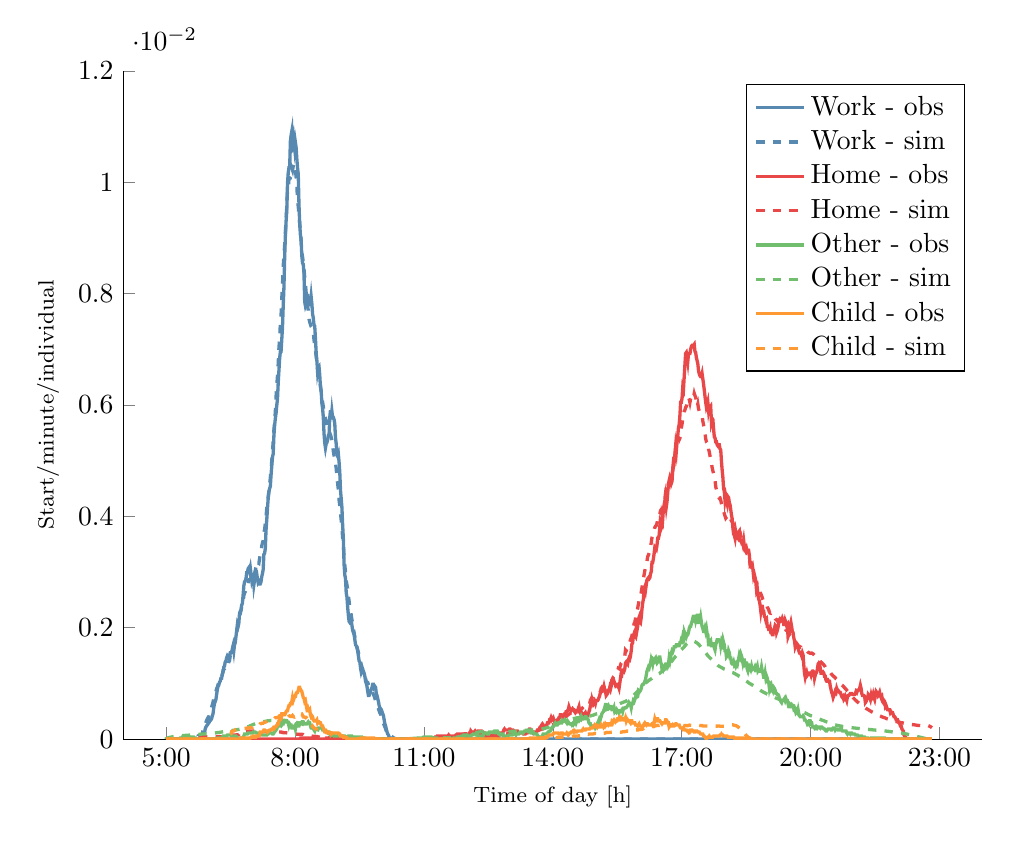
\begin{tikzpicture}

\begin{axis}[%
width=0.9\textwidth,
height=0.7\textwidth,
at={(0in,0in)},
scale only axis,
xmin=4,
xmax=24,
xtick={ 5,  8, 11, 14, 17, 20, 23},
xlabel style={font=\footnotesize},
xlabel={Time of day [h]},
ymin=0,
ymax=0.012,
ylabel style={font=\footnotesize},
ylabel={Start/minute/individual},
%axis background/.style={fill=white},
axis x line*=bottom,
axis y line*=left,
legend style={legend cell align=left, align=left},
every axis plot/.append style = {very thick},
xticklabels={5:00,8:00,11:00,14:00,17:00,20:00,23:00}
]
\addplot [color=mycolor1]
  table[row sep=crcr]{%
5	0\\
5.00083333333333	0\\
5.0025	0\\
5.005	0\\
5.00833333333333	0\\
5.0125	0\\
5.0175	0\\
5.02333333333333	0\\
5.03	0\\
5.0375	0\\
5.04583333333333	0\\
5.055	0\\
5.065	0\\
5.07583333333333	0\\
5.0875	0\\
5.1	0\\
5.11333333333333	0\\
5.1275	0\\
5.1425	0\\
5.15833333333333	0\\
5.175	0\\
5.19166666666667	0\\
5.20833333333333	0\\
5.225	0\\
5.24166666666667	0\\
5.25833333333333	0\\
5.275	0\\
5.29166666666667	0\\
5.30833333333333	0\\
5.325	0\\
5.34166666666667	0\\
5.35833333333333	0\\
5.375	0\\
5.39166666666667	0\\
5.40833333333333	0\\
5.425	0\\
5.44166666666667	0\\
5.45833333333333	0\\
5.475	0\\
5.49166666666667	0\\
5.50833333333333	0\\
5.525	0\\
5.54166666666667	0\\
5.55833333333333	0\\
5.575	0\\
5.59166666666667	0\\
5.60833333333333	0\\
5.625	0\\
5.64166666666667	0\\
5.65833333333333	0\\
5.675	0\\
5.69166666666667	0\\
5.70833333333333	0\\
5.725	0\\
5.74166666666667	0\\
5.75833333333333	0\\
5.775	0\\
5.79166666666667	0\\
5.80833333333333	1.82215743440233e-05\\
5.825	1.82215743440233e-05\\
5.84166666666667	3.64431486880466e-05\\
5.85833333333333	7.28862973760933e-05\\
5.875	7.28862973760933e-05\\
5.89166666666667	9.11078717201166e-05\\
5.90833333333333	0.000182215743440233\\
5.925	0.00021865889212828\\
5.94166666666667	0.000236880466472303\\
5.95833333333333	0.000255102040816327\\
5.975	0.00027332361516035\\
5.99166666666667	0.000291545189504373\\
6.00833333333333	0.000309766763848396\\
6.025	0.000346209912536443\\
6.04166666666667	0.000346209912536443\\
6.05833333333333	0.000364431486880466\\
6.075	0.000419096209912536\\
6.09166666666667	0.000455539358600583\\
6.10833333333333	0.000564868804664723\\
6.125	0.000637755102040816\\
6.14166666666667	0.000674198250728863\\
6.15833333333333	0.00071064139941691\\
6.175	0.000801749271137026\\
6.19166666666667	0.000892857142857143\\
6.20833333333333	0.000947521865889213\\
6.225	0.000965743440233236\\
6.24166666666667	0.00102040816326531\\
6.25833333333333	0.00103862973760933\\
6.275	0.0010932944606414\\
6.29166666666667	0.0010932944606414\\
6.30833333333333	0.00116618075801749\\
6.325	0.00120262390670554\\
6.34166666666667	0.00129373177842566\\
6.35833333333333	0.00131195335276968\\
6.375	0.00138483965014577\\
6.39166666666667	0.0014030612244898\\
6.40833333333333	0.00145772594752187\\
6.425	0.00149416909620991\\
6.44166666666667	0.00147594752186589\\
6.45833333333333	0.00147594752186589\\
6.475	0.00149416909620991\\
6.49166666666667	0.00154883381924198\\
6.50833333333333	0.00154883381924198\\
6.525	0.00156705539358601\\
6.54166666666667	0.00162172011661808\\
6.55833333333333	0.00167638483965015\\
6.575	0.00158527696793003\\
6.59166666666667	0.00169460641399417\\
6.60833333333333	0.00173104956268222\\
6.625	0.00184037900874636\\
6.64166666666667	0.0019497084548105\\
6.65833333333333	0.00205903790087464\\
6.675	0.00202259475218659\\
6.69166666666667	0.00207725947521866\\
6.70833333333333	0.00225947521865889\\
6.725	0.00229591836734694\\
6.74166666666667	0.00231413994169096\\
6.75833333333333	0.00240524781341108\\
6.775	0.00244169096209913\\
6.79166666666667	0.00258746355685131\\
6.80833333333333	0.00275145772594752\\
6.825	0.00282434402332362\\
6.84166666666667	0.00284256559766764\\
6.85833333333333	0.00287900874635569\\
6.875	0.00298833819241983\\
6.89166666666667	0.00298833819241983\\
6.90833333333333	0.00306122448979592\\
6.925	0.00307944606413994\\
6.94166666666667	0.00302478134110787\\
6.95833333333333	0.00307944606413994\\
6.975	0.0029701166180758\\
6.99166666666667	0.00286078717201166\\
7.00833333333333	0.00291545189504373\\
7.025	0.00293367346938776\\
7.04166666666667	0.00276967930029155\\
7.05833333333333	0.00286078717201166\\
7.075	0.00289723032069971\\
7.09166666666667	0.00295189504373178\\
7.10833333333333	0.0029701166180758\\
7.125	0.00287900874635569\\
7.14166666666667	0.00280612244897959\\
7.15833333333333	0.00282434402332362\\
7.175	0.00278790087463557\\
7.19166666666667	0.00278790087463557\\
7.20833333333333	0.00282434402332362\\
7.225	0.00291545189504373\\
7.24166666666667	0.0029701166180758\\
7.25833333333333	0.00304300291545189\\
7.275	0.00331632653061224\\
7.29166666666667	0.00333454810495627\\
7.30833333333333	0.00342565597667638\\
7.325	0.00375364431486881\\
7.34166666666667	0.00393586005830904\\
7.35833333333333	0.00413629737609329\\
7.375	0.00431851311953353\\
7.39166666666667	0.00444606413994169\\
7.40833333333333	0.00450072886297376\\
7.425	0.00453717201166181\\
7.44166666666667	0.00473760932944606\\
7.45833333333333	0.00490160349854227\\
7.475	0.00506559766763848\\
7.49166666666667	0.00512026239067055\\
7.50833333333333	0.00544825072886297\\
7.525	0.00563046647230321\\
7.54166666666667	0.00575801749271137\\
7.55833333333333	0.00584912536443149\\
7.575	0.00599489795918367\\
7.59166666666667	0.00610422740524781\\
7.60833333333333	0.00639577259475219\\
7.625	0.00661443148688047\\
7.64166666666667	0.00683309037900875\\
7.65833333333333	0.00696064139941691\\
7.675	0.00696064139941691\\
7.69166666666667	0.00717930029154519\\
7.70833333333333	0.00739795918367347\\
7.725	0.00778061224489796\\
7.74166666666667	0.00810860058309038\\
7.75833333333333	0.00863702623906706\\
7.775	0.00903790087463557\\
7.79166666666667	0.00929300291545189\\
7.80833333333333	0.00949344023323615\\
7.825	0.00998542274052478\\
7.84166666666667	0.010167638483965\\
7.85833333333333	0.0102587463556851\\
7.875	0.0102587463556851\\
7.89166666666667	0.0107325072886297\\
7.90833333333333	0.0108418367346939\\
7.925	0.01091472303207\\
7.94166666666667	0.0105867346938776\\
7.95833333333333	0.0106049562682216\\
7.975	0.0107325072886297\\
7.99166666666667	0.0106049562682216\\
8.00833333333333	0.0107142857142857\\
8.025	0.0106231778425656\\
8.04166666666667	0.0104227405247813\\
8.05833333333333	0.0102587463556851\\
8.075	0.010149416909621\\
8.09166666666667	0.00960276967930029\\
8.10833333333333	0.00925655976676385\\
8.125	0.00905612244897959\\
8.14166666666667	0.00896501457725947\\
8.15833333333333	0.0086734693877551\\
8.175	0.00854591836734694\\
8.19166666666667	0.00852769679300291\\
8.20833333333333	0.0083637026239067\\
8.225	0.00785349854227405\\
8.24166666666667	0.00778061224489796\\
8.25833333333333	0.00781705539358601\\
8.275	0.00796282798833819\\
8.29166666666667	0.00796282798833819\\
8.30833333333333	0.00781705539358601\\
8.325	0.00779883381924198\\
8.34166666666667	0.00779883381924198\\
8.35833333333333	0.00781705539358601\\
8.375	0.00794460641399417\\
8.39166666666667	0.00781705539358601\\
8.40833333333333	0.00763483965014577\\
8.425	0.00756195335276968\\
8.44166666666667	0.00743440233236152\\
8.45833333333333	0.00741618075801749\\
8.475	0.00719752186588921\\
8.49166666666667	0.00694241982507289\\
8.50833333333333	0.0067966472303207\\
8.525	0.00659620991253644\\
8.54166666666667	0.00666909620991254\\
8.55833333333333	0.00668731778425656\\
8.575	0.00654154518950437\\
8.59166666666667	0.00632288629737609\\
8.60833333333333	0.00625\\
8.625	0.00603134110787172\\
8.64166666666667	0.0059402332361516\\
8.65833333333333	0.00577623906705539\\
8.675	0.00548469387755102\\
8.69166666666667	0.00532069970845481\\
8.70833333333333	0.00522959183673469\\
8.725	0.00530247813411079\\
8.74166666666667	0.00532069970845481\\
8.75833333333333	0.00537536443148688\\
8.775	0.00544825072886297\\
8.79166666666667	0.00544825072886297\\
8.80833333333333	0.00577623906705539\\
8.825	0.00590379008746356\\
8.84166666666667	0.00573979591836735\\
8.85833333333333	0.00588556851311953\\
8.875	0.00577623906705539\\
8.89166666666667	0.00577623906705539\\
8.90833333333333	0.00573979591836735\\
8.925	0.00566690962099125\\
8.94166666666667	0.00541180758017493\\
8.95833333333333	0.00530247813411079\\
8.975	0.00512026239067055\\
8.99166666666667	0.00508381924198251\\
9.00833333333333	0.00512026239067055\\
9.025	0.00497448979591837\\
9.04166666666667	0.00479227405247813\\
9.05833333333333	0.00446428571428571\\
9.075	0.00431851311953353\\
9.09166666666667	0.00415451895043732\\
9.10833333333333	0.00384475218658892\\
9.125	0.00358965014577259\\
9.14166666666667	0.00313411078717201\\
9.15833333333333	0.00295189504373178\\
9.175	0.00287900874635569\\
9.19166666666667	0.00262390670553936\\
9.20833333333333	0.00255102040816327\\
9.225	0.00236880466472303\\
9.24166666666667	0.00222303206997085\\
9.25833333333333	0.00211370262390671\\
9.275	0.00209548104956268\\
9.29166666666667	0.00211370262390671\\
9.30833333333333	0.00213192419825073\\
9.325	0.00204081632653061\\
9.34166666666667	0.0019497084548105\\
9.35833333333333	0.00191326530612245\\
9.375	0.0018768221574344\\
9.39166666666667	0.00178571428571429\\
9.40833333333333	0.00169460641399417\\
9.425	0.00167638483965015\\
9.44166666666667	0.0016399416909621\\
9.45833333333333	0.00158527696793003\\
9.475	0.00149416909620991\\
9.49166666666667	0.0014030612244898\\
9.50833333333333	0.00138483965014577\\
9.525	0.00127551020408163\\
9.54166666666667	0.00120262390670554\\
9.55833333333333	0.00123906705539359\\
9.575	0.00123906705539359\\
9.59166666666667	0.00122084548104956\\
9.60833333333333	0.00118440233236152\\
9.625	0.00112973760932945\\
9.64166666666667	0.00103862973760933\\
9.65833333333333	0.00100218658892128\\
9.675	0.000947521865889213\\
9.69166666666667	0.000856413994169096\\
9.70833333333333	0.000783527696793003\\
9.725	0.000783527696793003\\
9.74166666666667	0.00081997084548105\\
9.75833333333333	0.000856413994169096\\
9.775	0.000892857142857143\\
9.79166666666667	0.000929300291545189\\
9.80833333333333	0.00098396501457726\\
9.825	0.00098396501457726\\
9.84166666666667	0.000929300291545189\\
9.85833333333333	0.000947521865889213\\
9.875	0.000929300291545189\\
9.89166666666667	0.00081997084548105\\
9.90833333333333	0.000783527696793003\\
9.925	0.000728862973760933\\
9.94166666666667	0.000674198250728863\\
9.95833333333333	0.00060131195335277\\
9.975	0.000564868804664723\\
9.99166666666667	0.0005466472303207\\
10.0083333333333	0.000528425655976676\\
10.025	0.00049198250728863\\
10.0416666666667	0.000455539358600583\\
10.0583333333333	0.000419096209912536\\
10.075	0.000346209912536443\\
10.0916666666667	0.00027332361516035\\
10.1083333333333	0.000236880466472303\\
10.125	0.000182215743440233\\
10.1416666666667	0.000127551020408163\\
10.1583333333333	9.11078717201166e-05\\
10.175	7.28862973760933e-05\\
10.1916666666667	3.64431486880466e-05\\
10.2083333333333	1.82215743440233e-05\\
10.225	1.82215743440233e-05\\
10.2416666666667	1.82215743440233e-05\\
10.2583333333333	1.82215743440233e-05\\
10.275	1.82215743440233e-05\\
10.2916666666667	1.82215743440233e-05\\
10.3083333333333	1.82215743440233e-05\\
10.325	0\\
10.3416666666667	0\\
10.3583333333333	0\\
10.375	0\\
10.3916666666667	0\\
10.4083333333333	0\\
10.425	0\\
10.4416666666667	0\\
10.4583333333333	0\\
10.475	0\\
10.4916666666667	0\\
10.5083333333333	0\\
10.525	0\\
10.5416666666667	0\\
10.5583333333333	0\\
10.575	0\\
10.5916666666667	0\\
10.6083333333333	0\\
10.625	0\\
10.6416666666667	0\\
10.6583333333333	0\\
10.675	0\\
10.6916666666667	0\\
10.7083333333333	0\\
10.725	0\\
10.7416666666667	0\\
10.7583333333333	0\\
10.775	0\\
10.7916666666667	0\\
10.8083333333333	0\\
10.825	0\\
10.8416666666667	0\\
10.8583333333333	0\\
10.875	0\\
10.8916666666667	0\\
10.9083333333333	0\\
10.925	0\\
10.9416666666667	0\\
10.9583333333333	0\\
10.975	1.82215743440233e-05\\
10.9916666666667	1.82215743440233e-05\\
11.0083333333333	1.82215743440233e-05\\
11.025	1.82215743440233e-05\\
11.0416666666667	1.82215743440233e-05\\
11.0583333333333	1.82215743440233e-05\\
11.075	1.82215743440233e-05\\
11.0916666666667	1.82215743440233e-05\\
11.1083333333333	1.82215743440233e-05\\
11.125	1.82215743440233e-05\\
11.1416666666667	1.82215743440233e-05\\
11.1583333333333	1.82215743440233e-05\\
11.175	1.82215743440233e-05\\
11.1916666666667	1.82215743440233e-05\\
11.2083333333333	1.82215743440233e-05\\
11.225	1.82215743440233e-05\\
11.2416666666667	1.82215743440233e-05\\
11.2583333333333	1.82215743440233e-05\\
11.275	1.82215743440233e-05\\
11.2916666666667	1.82215743440233e-05\\
11.3083333333333	0\\
11.325	0\\
11.3416666666667	0\\
11.3583333333333	0\\
11.375	0\\
11.3916666666667	0\\
11.4083333333333	0\\
11.425	0\\
11.4416666666667	0\\
11.4583333333333	0\\
11.475	0\\
11.4916666666667	0\\
11.5083333333333	0\\
11.525	0\\
11.5416666666667	0\\
11.5583333333333	0\\
11.575	0\\
11.5916666666667	0\\
11.6083333333333	0\\
11.625	0\\
11.6416666666667	0\\
11.6583333333333	0\\
11.675	0\\
11.6916666666667	0\\
11.7083333333333	0\\
11.725	0\\
11.7416666666667	0\\
11.7583333333333	0\\
11.775	0\\
11.7916666666667	0\\
11.8083333333333	0\\
11.825	0\\
11.8416666666667	0\\
11.8583333333333	0\\
11.875	0\\
11.8916666666667	0\\
11.9083333333333	0\\
11.925	0\\
11.9416666666667	0\\
11.9583333333333	0\\
11.975	0\\
11.9916666666667	0\\
12.0083333333333	0\\
12.025	0\\
12.0416666666667	0\\
12.0583333333333	0\\
12.075	0\\
12.0916666666667	0\\
12.1083333333333	0\\
12.125	0\\
12.1416666666667	0\\
12.1583333333333	0\\
12.175	0\\
12.1916666666667	0\\
12.2083333333333	0\\
12.225	0\\
12.2416666666667	0\\
12.2583333333333	0\\
12.275	0\\
12.2916666666667	0\\
12.3083333333333	0\\
12.325	0\\
12.3416666666667	0\\
12.3583333333333	0\\
12.375	0\\
12.3916666666667	0\\
12.4083333333333	0\\
12.425	0\\
12.4416666666667	0\\
12.4583333333333	0\\
12.475	0\\
12.4916666666667	0\\
12.5083333333333	0\\
12.525	0\\
12.5416666666667	0\\
12.5583333333333	0\\
12.575	0\\
12.5916666666667	0\\
12.6083333333333	0\\
12.625	0\\
12.6416666666667	0\\
12.6583333333333	0\\
12.675	0\\
12.6916666666667	0\\
12.7083333333333	0\\
12.725	0\\
12.7416666666667	0\\
12.7583333333333	0\\
12.775	0\\
12.7916666666667	0\\
12.8083333333333	0\\
12.825	0\\
12.8416666666667	0\\
12.8583333333333	0\\
12.875	0\\
12.8916666666667	0\\
12.9083333333333	0\\
12.925	0\\
12.9416666666667	0\\
12.9583333333333	0\\
12.975	0\\
12.9916666666667	0\\
13.0083333333333	0\\
13.025	0\\
13.0416666666667	0\\
13.0583333333333	0\\
13.075	0\\
13.0916666666667	0\\
13.1083333333333	0\\
13.125	0\\
13.1416666666667	0\\
13.1583333333333	0\\
13.175	0\\
13.1916666666667	0\\
13.2083333333333	0\\
13.225	0\\
13.2416666666667	0\\
13.2583333333333	0\\
13.275	0\\
13.2916666666667	0\\
13.3083333333333	0\\
13.325	0\\
13.3416666666667	0\\
13.3583333333333	0\\
13.375	0\\
13.3916666666667	0\\
13.4083333333333	0\\
13.425	0\\
13.4416666666667	0\\
13.4583333333333	0\\
13.475	0\\
13.4916666666667	0\\
13.5083333333333	0\\
13.525	0\\
13.5416666666667	0\\
13.5583333333333	0\\
13.575	0\\
13.5916666666667	0\\
13.6083333333333	0\\
13.625	0\\
13.6416666666667	0\\
13.6583333333333	0\\
13.675	0\\
13.6916666666667	0\\
13.7083333333333	0\\
13.725	0\\
13.7416666666667	0\\
13.7583333333333	0\\
13.775	0\\
13.7916666666667	0\\
13.8083333333333	0\\
13.825	0\\
13.8416666666667	0\\
13.8583333333333	0\\
13.875	0\\
13.8916666666667	0\\
13.9083333333333	0\\
13.925	0\\
13.9416666666667	0\\
13.9583333333333	0\\
13.975	0\\
13.9916666666667	0\\
14.0083333333333	0\\
14.025	0\\
14.0416666666667	0\\
14.0583333333333	0\\
14.075	0\\
14.0916666666667	0\\
14.1083333333333	0\\
14.125	0\\
14.1416666666667	0\\
14.1583333333333	0\\
14.175	0\\
14.1916666666667	0\\
14.2083333333333	0\\
14.225	0\\
14.2416666666667	0\\
14.2583333333333	0\\
14.275	0\\
14.2916666666667	0\\
14.3083333333333	0\\
14.325	0\\
14.3416666666667	0\\
14.3583333333333	0\\
14.375	0\\
14.3916666666667	0\\
14.4083333333333	0\\
14.425	0\\
14.4416666666667	0\\
14.4583333333333	0\\
14.475	0\\
14.4916666666667	0\\
14.5083333333333	0\\
14.525	0\\
14.5416666666667	0\\
14.5583333333333	0\\
14.575	0\\
14.5916666666667	0\\
14.6083333333333	0\\
14.625	0\\
14.6416666666667	0\\
14.6583333333333	0\\
14.675	0\\
14.6916666666667	0\\
14.7083333333333	0\\
14.725	0\\
14.7416666666667	0\\
14.7583333333333	0\\
14.775	0\\
14.7916666666667	0\\
14.8083333333333	0\\
14.825	0\\
14.8416666666667	0\\
14.8583333333333	0\\
14.875	0\\
14.8916666666667	0\\
14.9083333333333	0\\
14.925	0\\
14.9416666666667	0\\
14.9583333333333	0\\
14.975	0\\
14.9916666666667	0\\
15.0083333333333	0\\
15.025	0\\
15.0416666666667	0\\
15.0583333333333	0\\
15.075	0\\
15.0916666666667	0\\
15.1083333333333	0\\
15.125	0\\
15.1416666666667	0\\
15.1583333333333	0\\
15.175	0\\
15.1916666666667	0\\
15.2083333333333	0\\
15.225	0\\
15.2416666666667	0\\
15.2583333333333	0\\
15.275	0\\
15.2916666666667	0\\
15.3083333333333	0\\
15.325	0\\
15.3416666666667	0\\
15.3583333333333	0\\
15.375	0\\
15.3916666666667	0\\
15.4083333333333	0\\
15.425	0\\
15.4416666666667	0\\
15.4583333333333	0\\
15.475	0\\
15.4916666666667	0\\
15.5083333333333	0\\
15.525	0\\
15.5416666666667	0\\
15.5583333333333	0\\
15.575	0\\
15.5916666666667	0\\
15.6083333333333	0\\
15.625	0\\
15.6416666666667	0\\
15.6583333333333	0\\
15.675	0\\
15.6916666666667	0\\
15.7083333333333	0\\
15.725	0\\
15.7416666666667	0\\
15.7583333333333	0\\
15.775	0\\
15.7916666666667	0\\
15.8083333333333	0\\
15.825	0\\
15.8416666666667	0\\
15.8583333333333	0\\
15.875	0\\
15.8916666666667	0\\
15.9083333333333	0\\
15.925	0\\
15.9416666666667	0\\
15.9583333333333	0\\
15.975	0\\
15.9916666666667	0\\
16.0083333333333	0\\
16.025	0\\
16.0416666666667	0\\
16.0583333333333	0\\
16.075	0\\
16.0916666666667	0\\
16.1083333333333	0\\
16.125	0\\
16.1416666666667	0\\
16.1583333333333	0\\
16.175	0\\
16.1916666666667	0\\
16.2083333333333	0\\
16.225	0\\
16.2416666666667	0\\
16.2583333333333	0\\
16.275	0\\
16.2916666666667	0\\
16.3083333333333	0\\
16.325	0\\
16.3416666666667	0\\
16.3583333333333	0\\
16.375	0\\
16.3916666666667	0\\
16.4083333333333	0\\
16.425	0\\
16.4416666666667	0\\
16.4583333333333	0\\
16.475	0\\
16.4916666666667	0\\
16.5083333333333	0\\
16.525	0\\
16.5416666666667	0\\
16.5583333333333	0\\
16.575	0\\
16.5916666666667	0\\
16.6083333333333	0\\
16.625	0\\
16.6416666666667	0\\
16.6583333333333	0\\
16.675	0\\
16.6916666666667	0\\
16.7083333333333	0\\
16.725	0\\
16.7416666666667	0\\
16.7583333333333	0\\
16.775	0\\
16.7916666666667	0\\
16.8083333333333	0\\
16.825	0\\
16.8416666666667	0\\
16.8583333333333	0\\
16.875	0\\
16.8916666666667	0\\
16.9083333333333	0\\
16.925	0\\
16.9416666666667	0\\
16.9583333333333	0\\
16.975	0\\
16.9916666666667	0\\
17.0083333333333	0\\
17.025	0\\
17.0416666666667	0\\
17.0583333333333	0\\
17.075	0\\
17.0916666666667	0\\
17.1083333333333	0\\
17.125	0\\
17.1416666666667	0\\
17.1583333333333	0\\
17.175	0\\
17.1916666666667	0\\
17.2083333333333	0\\
17.225	0\\
17.2416666666667	0\\
17.2583333333333	0\\
17.275	0\\
17.2916666666667	0\\
17.3083333333333	0\\
17.325	0\\
17.3416666666667	0\\
17.3583333333333	0\\
17.375	0\\
17.3916666666667	0\\
17.4083333333333	0\\
17.425	0\\
17.4416666666667	0\\
17.4583333333333	0\\
17.475	0\\
17.4916666666667	0\\
17.5083333333333	0\\
17.525	0\\
17.5416666666667	0\\
17.5583333333333	0\\
17.575	0\\
17.5916666666667	0\\
17.6083333333333	0\\
17.625	0\\
17.6416666666667	0\\
17.6583333333333	0\\
17.675	0\\
17.6916666666667	0\\
17.7083333333333	0\\
17.725	0\\
17.7416666666667	0\\
17.7583333333333	0\\
17.775	0\\
17.7916666666667	0\\
17.8083333333333	0\\
17.825	0\\
17.8416666666667	0\\
17.8583333333333	0\\
17.875	0\\
17.8916666666667	0\\
17.9083333333333	0\\
17.925	0\\
17.9416666666667	0\\
17.9583333333333	0\\
17.975	0\\
17.9916666666667	0\\
18.0083333333333	0\\
18.025	0\\
18.0416666666667	0\\
18.0583333333333	0\\
18.075	0\\
18.0916666666667	0\\
18.1083333333333	0\\
18.125	0\\
18.1416666666667	0\\
18.1583333333333	0\\
18.175	0\\
18.1916666666667	0\\
18.2083333333333	0\\
18.225	0\\
18.2416666666667	0\\
18.2583333333333	0\\
18.275	0\\
18.2916666666667	0\\
18.3083333333333	0\\
18.325	0\\
18.3416666666667	0\\
18.3583333333333	0\\
18.375	0\\
18.3916666666667	0\\
18.4083333333333	0\\
18.425	0\\
18.4416666666667	0\\
18.4583333333333	0\\
18.475	0\\
18.4916666666667	0\\
18.5083333333333	0\\
18.525	0\\
18.5416666666667	0\\
18.5583333333333	0\\
18.575	0\\
18.5916666666667	0\\
18.6083333333333	0\\
18.625	0\\
18.6416666666667	0\\
18.6583333333333	0\\
18.675	0\\
18.6916666666667	0\\
18.7083333333333	0\\
18.725	0\\
18.7416666666667	0\\
18.7583333333333	0\\
18.775	0\\
18.7916666666667	0\\
18.8083333333333	0\\
18.825	0\\
18.8416666666667	0\\
18.8583333333333	0\\
18.875	0\\
18.8916666666667	0\\
18.9083333333333	0\\
18.925	0\\
18.9416666666667	0\\
18.9583333333333	0\\
18.975	0\\
18.9916666666667	0\\
19.0083333333333	0\\
19.025	0\\
19.0416666666667	0\\
19.0583333333333	0\\
19.075	0\\
19.0916666666667	0\\
19.1083333333333	0\\
19.125	0\\
19.1416666666667	0\\
19.1583333333333	0\\
19.175	0\\
19.1916666666667	0\\
19.2083333333333	0\\
19.225	0\\
19.2416666666667	0\\
19.2583333333333	0\\
19.275	0\\
19.2916666666667	0\\
19.3083333333333	0\\
19.325	0\\
19.3416666666667	0\\
19.3583333333333	0\\
19.375	0\\
19.3916666666667	0\\
19.4083333333333	0\\
19.425	0\\
19.4416666666667	0\\
19.4583333333333	0\\
19.475	0\\
19.4916666666667	0\\
19.5083333333333	0\\
19.525	0\\
19.5416666666667	0\\
19.5583333333333	0\\
19.575	0\\
19.5916666666667	0\\
19.6083333333333	0\\
19.625	0\\
19.6416666666667	0\\
19.6583333333333	0\\
19.675	0\\
19.6916666666667	0\\
19.7083333333333	0\\
19.725	0\\
19.7416666666667	0\\
19.7583333333333	0\\
19.775	0\\
19.7916666666667	0\\
19.8083333333333	0\\
19.825	0\\
19.8416666666667	0\\
19.8583333333333	0\\
19.875	0\\
19.8916666666667	0\\
19.9083333333333	0\\
19.925	0\\
19.9416666666667	0\\
19.9583333333333	0\\
19.975	0\\
19.9916666666667	0\\
20.0083333333333	0\\
20.025	0\\
20.0416666666667	0\\
20.0583333333333	0\\
20.075	0\\
20.0916666666667	0\\
20.1083333333333	0\\
20.125	0\\
20.1416666666667	0\\
20.1583333333333	0\\
20.175	0\\
20.1916666666667	0\\
20.2083333333333	0\\
20.225	0\\
20.2416666666667	0\\
20.2583333333333	0\\
20.275	0\\
20.2916666666667	0\\
20.3083333333333	0\\
20.325	0\\
20.3416666666667	0\\
20.3583333333333	0\\
20.375	0\\
20.3916666666667	0\\
20.4083333333333	0\\
20.425	0\\
20.4416666666667	0\\
20.4583333333333	0\\
20.475	0\\
20.4916666666667	0\\
20.5083333333333	0\\
20.525	0\\
20.5416666666667	0\\
20.5583333333333	0\\
20.575	0\\
20.5916666666667	0\\
20.6083333333333	0\\
20.625	0\\
20.6416666666667	0\\
20.6583333333333	0\\
20.675	0\\
20.6916666666667	0\\
20.7083333333333	0\\
20.725	0\\
20.7416666666667	0\\
20.7583333333333	0\\
20.775	0\\
20.7916666666667	0\\
20.8083333333333	0\\
20.825	0\\
20.8416666666667	0\\
20.8583333333333	0\\
20.875	0\\
20.8916666666667	0\\
20.9083333333333	0\\
20.925	0\\
20.9416666666667	0\\
20.9583333333333	0\\
20.975	0\\
20.9916666666667	0\\
21.0083333333333	0\\
21.025	0\\
21.0416666666667	0\\
21.0583333333333	0\\
21.075	0\\
21.0916666666667	0\\
21.1083333333333	0\\
21.125	0\\
21.1416666666667	0\\
21.1583333333333	0\\
21.175	0\\
21.1916666666667	0\\
21.2083333333333	0\\
21.225	0\\
21.2416666666667	0\\
21.2583333333333	0\\
21.275	0\\
21.2916666666667	0\\
21.3083333333333	0\\
21.325	0\\
21.3416666666667	0\\
21.3583333333333	0\\
21.375	0\\
21.3916666666667	0\\
21.4083333333333	0\\
21.425	0\\
21.4416666666667	0\\
21.4583333333333	0\\
21.475	0\\
21.4916666666667	0\\
21.5083333333333	0\\
21.525	0\\
21.5416666666667	0\\
21.5583333333333	0\\
21.575	0\\
21.5916666666667	0\\
21.6083333333333	0\\
21.625	0\\
21.6416666666667	0\\
21.6583333333333	0\\
21.675	0\\
21.6916666666667	0\\
21.7083333333333	0\\
21.725	0\\
21.7416666666667	0\\
21.7583333333333	0\\
21.775	0\\
21.7916666666667	0\\
21.8083333333333	0\\
21.825	0\\
21.8416666666667	0\\
21.8583333333333	0\\
21.875	0\\
21.8916666666667	0\\
21.9083333333333	0\\
21.925	0\\
21.9416666666667	0\\
21.9583333333333	0\\
21.975	0\\
21.9916666666667	0\\
22.0083333333333	0\\
22.025	0\\
22.0416666666667	0\\
22.0583333333333	0\\
22.075	0\\
22.0916666666667	0\\
22.1083333333333	0\\
22.125	0\\
22.1416666666667	0\\
22.1583333333333	0\\
22.175	0\\
22.1916666666667	0\\
22.2083333333333	0\\
22.225	0\\
22.2416666666667	0\\
22.2583333333333	0\\
22.275	0\\
22.2916666666667	0\\
22.3083333333333	0\\
22.325	0\\
22.3416666666667	0\\
22.3583333333333	0\\
22.375	0\\
22.3916666666667	0\\
22.4083333333333	0\\
22.425	0\\
22.4416666666667	0\\
22.4583333333333	0\\
22.475	0\\
22.4916666666667	0\\
22.5083333333333	0\\
22.525	0\\
22.5416666666667	0\\
22.5583333333333	0\\
22.575	0\\
22.5916666666667	0\\
22.6083333333333	0\\
22.625	0\\
22.6416666666667	0\\
22.6583333333333	0\\
22.675	0\\
22.6916666666667	0\\
22.7083333333333	0\\
22.725	0\\
22.7416666666667	0\\
22.7583333333333	0\\
22.775	0\\
22.7916666666667	0\\
22.8083333333333	0\\
22.825	0\\
};
\addlegendentry{Work - obs}

\addplot [color=mycolor1, dashed]
  table[row sep=crcr]{%
5	0\\
5.00083333333333	0\\
5.0025	0\\
5.005	0\\
5.00833333333333	0\\
5.0125	0\\
5.0175	0\\
5.02333333333333	0\\
5.03	0\\
5.0375	0\\
5.04583333333333	0\\
5.055	0\\
5.065	0\\
5.07583333333333	0\\
5.0875	0\\
5.1	0\\
5.11333333333333	0\\
5.1275	0\\
5.1425	0\\
5.15833333333333	0\\
5.175	0\\
5.19166666666667	0\\
5.20833333333333	0\\
5.225	0\\
5.24166666666667	0\\
5.25833333333333	0\\
5.275	0\\
5.29166666666667	0\\
5.30833333333333	0\\
5.325	0\\
5.34166666666667	0\\
5.35833333333333	0\\
5.375	0\\
5.39166666666667	0\\
5.40833333333333	0\\
5.425	0\\
5.44166666666667	0\\
5.45833333333333	0\\
5.475	0\\
5.49166666666667	0\\
5.50833333333333	0\\
5.525	0\\
5.54166666666667	0\\
5.55833333333333	0\\
5.575	0\\
5.59166666666667	0\\
5.60833333333333	0\\
5.625	0\\
5.64166666666667	0\\
5.65833333333333	9.11078717201166e-08\\
5.675	1.51846452866861e-07\\
5.69166666666667	1.70675413022352e-05\\
5.70833333333333	2.37184159378037e-05\\
5.725	2.95796890184645e-05\\
5.74166666666667	5.8096452866861e-05\\
5.75833333333333	6.44740038872692e-05\\
5.775	6.95760447035957e-05\\
5.79166666666667	7.55284256559767e-05\\
5.80833333333333	8.14200680272109e-05\\
5.825	8.39710884353741e-05\\
5.84166666666667	0.000106960641399417\\
5.85833333333333	0.000155004859086492\\
5.875	0.000172862001943635\\
5.89166666666667	0.000196732264334305\\
5.90833333333333	0.000265640184645287\\
5.925	0.000298530126336249\\
5.94166666666667	0.000334942905733722\\
5.95833333333333	0.000362761175898931\\
5.975	0.000386479591836735\\
5.99166666666667	0.000401967930029155\\
6.00833333333333	0.000457422254616132\\
6.025	0.000510143343051506\\
6.04166666666667	0.00053088556851312\\
6.05833333333333	0.000571975218658892\\
6.075	0.000617316569484937\\
6.09166666666667	0.000664328231292517\\
6.10833333333333	0.000728954081632653\\
6.125	0.000767523080660836\\
6.14166666666667	0.000814018464528669\\
6.15833333333333	0.000852405247813411\\
6.175	0.000906037414965986\\
6.19166666666667	0.000935617103984451\\
6.20833333333333	0.000980594023323615\\
6.225	0.00101236030126336\\
6.24166666666667	0.00103334548104956\\
6.25833333333333	0.00105654761904762\\
6.275	0.00107665208940719\\
6.29166666666667	0.00112697400388727\\
6.30833333333333	0.00116147351797862\\
6.325	0.00123530126336249\\
6.34166666666667	0.00125012147716229\\
6.35833333333333	0.0012626639941691\\
6.375	0.00132756316812439\\
6.39166666666667	0.00132710762876579\\
6.40833333333333	0.0013189990281827\\
6.425	0.0013316630223518\\
6.44166666666667	0.00133965014577259\\
6.45833333333333	0.00138714771622935\\
6.475	0.00140576409135083\\
6.49166666666667	0.00149325801749271\\
6.50833333333333	0.0015228073372206\\
6.525	0.00157121598639456\\
6.54166666666667	0.00164619776482021\\
6.55833333333333	0.00166530004859086\\
6.575	0.0016799684159378\\
6.59166666666667	0.00172142249757046\\
6.60833333333333	0.00178626093294461\\
6.625	0.00182950680272109\\
6.64166666666667	0.00192343901846453\\
6.65833333333333	0.00198979591836735\\
6.675	0.00205296404275996\\
6.69166666666667	0.00213414115646259\\
6.70833333333333	0.00221771744412051\\
6.725	0.00224857264334305\\
6.74166666666667	0.00230961491739553\\
6.75833333333333	0.00236716472303207\\
6.775	0.00238988095238095\\
6.79166666666667	0.00246531827016521\\
6.80833333333333	0.0025756195335277\\
6.825	0.00262354227405248\\
6.84166666666667	0.00264938654033042\\
6.85833333333333	0.00268950437317784\\
6.875	0.00270617711370262\\
6.89166666666667	0.00274939261418853\\
6.90833333333333	0.00278844752186589\\
6.925	0.00286191083576288\\
6.94166666666667	0.00286121234207969\\
6.95833333333333	0.00287247934888241\\
6.975	0.00289337342079689\\
6.99166666666667	0.00285659620991254\\
7.00833333333333	0.00290069241982507\\
7.025	0.00289996355685131\\
7.04166666666667	0.00287846209912536\\
7.05833333333333	0.00298217322643343\\
7.075	0.00302918488824101\\
7.09166666666667	0.00309463070942663\\
7.10833333333333	0.00319333090379009\\
7.125	0.0031693695335277\\
7.14166666666667	0.00316265792031098\\
7.15833333333333	0.00315491375121477\\
7.175	0.00324413872691934\\
7.19166666666667	0.00332182337220602\\
7.20833333333333	0.00336145529640428\\
7.225	0.00346750485908649\\
7.24166666666667	0.00352156219630709\\
7.25833333333333	0.0035658102526725\\
7.275	0.00371194727891156\\
7.29166666666667	0.00376059888241011\\
7.30833333333333	0.00387178085519922\\
7.325	0.00399113216715258\\
7.34166666666667	0.00414218901846453\\
7.35833333333333	0.00425747084548105\\
7.375	0.00434715136054422\\
7.39166666666667	0.0044445760447036\\
7.40833333333333	0.00455943270165209\\
7.425	0.00469366496598639\\
7.44166666666667	0.00484314261418853\\
7.45833333333333	0.00499158770651118\\
7.475	0.00517079689018465\\
7.49166666666667	0.00533788872691934\\
7.50833333333333	0.00554947157434402\\
7.525	0.00569302721088435\\
7.54166666666667	0.00588584183673469\\
7.55833333333333	0.00614671404275996\\
7.575	0.00634794096209913\\
7.59166666666667	0.00652168367346939\\
7.60833333333333	0.00673514941690962\\
7.625	0.00701515427599611\\
7.64166666666667	0.00719454567541302\\
7.65833333333333	0.00745663265306123\\
7.675	0.0076142796404276\\
7.69166666666667	0.00791715257531584\\
7.70833333333333	0.00815081389698737\\
7.725	0.00848961370262391\\
7.74166666666667	0.00868422011661808\\
7.75833333333333	0.00886640549076774\\
7.775	0.00907777575315841\\
7.79166666666667	0.0093511601068999\\
7.80833333333333	0.00957419217687075\\
7.825	0.00985510811467444\\
7.84166666666667	0.00987336005830904\\
7.85833333333333	0.0100524781341108\\
7.875	0.0100813289601555\\
7.89166666666667	0.0100790208940719\\
7.90833333333333	0.0101356292517007\\
7.925	0.010249574829932\\
7.94166666666667	0.0102124635568513\\
7.95833333333333	0.0102910896501458\\
7.975	0.010332574101069\\
7.99166666666667	0.0103244655004859\\
8.00833333333333	0.0102264941690962\\
8.025	0.0100918671039845\\
8.04166666666667	0.00995402089407191\\
8.05833333333333	0.00966408527696793\\
8.075	0.00956574951409135\\
8.09166666666667	0.00939914358600583\\
8.10833333333333	0.00927204810495627\\
8.125	0.00910462220602527\\
8.14166666666667	0.00895034620991254\\
8.15833333333333	0.00873032069970845\\
8.175	0.0086636601068999\\
8.19166666666667	0.00855754980563654\\
8.20833333333333	0.00845001214771623\\
8.225	0.00829576652089407\\
8.24166666666667	0.00817957361516035\\
8.25833333333333	0.00802049927113703\\
8.275	0.00797063289601555\\
8.29166666666667	0.0077738398931001\\
8.30833333333333	0.00769733965014577\\
8.325	0.0075433369776482\\
8.34166666666667	0.00749243804664723\\
8.35833333333333	0.00744396865889213\\
8.375	0.00740706997084548\\
8.39166666666667	0.00738875728862974\\
8.40833333333333	0.00736330782312925\\
8.425	0.00729813532555879\\
8.44166666666667	0.00716903547133139\\
8.45833333333333	0.00706474732750243\\
8.475	0.00698785228377065\\
8.49166666666667	0.00687017128279883\\
8.50833333333333	0.00676445578231293\\
8.525	0.00664306972789116\\
8.54166666666667	0.00656918124392614\\
8.55833333333333	0.00652775753158406\\
8.575	0.00647370019436346\\
8.59166666666667	0.0063497934888241\\
8.60833333333333	0.00624076773566569\\
8.625	0.00616016763848397\\
8.64166666666667	0.0060540573372206\\
8.65833333333333	0.00596808187560739\\
8.675	0.00590154275996113\\
8.69166666666667	0.00584174562682216\\
8.70833333333333	0.00576466836734694\\
8.725	0.00572093658892128\\
8.74166666666667	0.00563547740524781\\
8.75833333333333	0.00558630952380952\\
8.775	0.00558889091350826\\
8.79166666666667	0.00554956268221574\\
8.80833333333333	0.0054963556851312\\
8.825	0.00546319241982507\\
8.84166666666667	0.00542018950437318\\
8.85833333333333	0.005354925898931\\
8.875	0.00529285106899903\\
8.89166666666667	0.00516760811467444\\
8.90833333333333	0.00509217079689018\\
8.925	0.00503006559766764\\
8.94166666666667	0.00495383867832847\\
8.95833333333333	0.00486385447035957\\
8.975	0.00468941326530612\\
8.99166666666667	0.00459684766763848\\
9.00833333333333	0.00447506681243926\\
9.025	0.00429048226433431\\
9.04166666666667	0.00419281462585034\\
9.05833333333333	0.00406146744412051\\
9.075	0.0039254130223518\\
9.09166666666667	0.00380235665694849\\
9.10833333333333	0.0036081146744412\\
9.125	0.00346838556851312\\
9.14166666666667	0.0032737184159378\\
9.15833333333333	0.00312518221574344\\
9.175	0.00299647716229349\\
9.19166666666667	0.00284381073858115\\
9.20833333333333	0.00276755344995141\\
9.225	0.00270080174927114\\
9.24166666666667	0.00257258260447036\\
9.25833333333333	0.00247852891156463\\
9.275	0.0023582361516035\\
9.29166666666667	0.00229874271137026\\
9.30833333333333	0.00222530976676385\\
9.325	0.00214425413022352\\
9.34166666666667	0.00206189261418853\\
9.35833333333333	0.00198022959183673\\
9.375	0.00191241496598639\\
9.39166666666667	0.00184037900874636\\
9.40833333333333	0.00176570092322643\\
9.425	0.00170362609329446\\
9.44166666666667	0.00165688775510204\\
9.45833333333333	0.00160225340136054\\
9.475	0.00155472546161322\\
9.49166666666667	0.00151011297376093\\
9.50833333333333	0.00145137876579203\\
9.525	0.00139079203109815\\
9.54166666666667	0.00134022716229349\\
9.55833333333333	0.00129351919339164\\
9.575	0.00126011297376093\\
9.59166666666667	0.00123250728862974\\
9.60833333333333	0.00118209426627794\\
9.625	0.00111977648202138\\
9.64166666666667	0.00108664358600583\\
9.65833333333333	0.00103890306122449\\
9.675	0.00101715864917396\\
9.69166666666667	0.00101731049562682\\
9.70833333333333	0.000983813168124393\\
9.725	0.000945851554907677\\
9.74166666666667	0.000915694849368319\\
9.75833333333333	0.000907252186588921\\
9.775	0.000875637755102041\\
9.79166666666667	0.000854713313896987\\
9.80833333333333	0.000831723760932945\\
9.825	0.000800230806608358\\
9.84166666666667	0.000771319241982507\\
9.85833333333333	0.000733327259475219\\
9.875	0.000688654033041788\\
9.89166666666667	0.000641217201166181\\
9.90833333333333	0.000595116618075802\\
9.925	0.000563896987366375\\
9.94166666666667	0.000545310981535471\\
9.95833333333333	0.000505284256559767\\
9.975	0.000469782555879495\\
9.99166666666667	0.000447643343051506\\
10.0083333333333	0.000404610058309038\\
10.025	0.000332817055393586\\
10.0416666666667	0.000305940233236152\\
10.0583333333333	0.000281978862973761\\
10.075	0.000248937074829932\\
10.0916666666667	0.000217990767735666\\
10.1083333333333	0.000184311224489796\\
10.125	0.000145347424684159\\
10.1416666666667	0.000118106171039845\\
10.1583333333333	9.70298833819242e-05\\
10.175	7.77453838678328e-05\\
10.1916666666667	5.52417395529641e-05\\
10.2083333333333	5.44521379980564e-05\\
10.225	5.36929057337221e-05\\
10.2416666666667	5.16885325558795e-05\\
10.2583333333333	4.67079689018465e-05\\
10.275	2.8152332361516e-05\\
10.2916666666667	1.75230806608358e-05\\
10.3083333333333	1.15403304178814e-05\\
10.325	2.70286686103013e-06\\
10.3416666666667	8.1997084548105e-07\\
10.3583333333333	8.1997084548105e-07\\
10.375	7.89601554907677e-07\\
10.3916666666667	8.1997084548105e-07\\
10.4083333333333	7.28862973760933e-07\\
10.425	7.28862973760933e-07\\
10.4416666666667	8.80709426627794e-07\\
10.4583333333333	8.80709426627794e-07\\
10.475	8.50340136054422e-07\\
10.4916666666667	8.1997084548105e-07\\
10.5083333333333	8.50340136054422e-07\\
10.525	9.11078717201166e-07\\
10.5416666666667	9.11078717201166e-07\\
10.5583333333333	9.11078717201166e-07\\
10.575	9.71817298347911e-07\\
10.5916666666667	9.71817298347911e-07\\
10.6083333333333	1.21477162293489e-06\\
10.625	1.24514091350826e-06\\
10.6416666666667	1.24514091350826e-06\\
10.6583333333333	1.24514091350826e-06\\
10.675	1.21477162293489e-06\\
10.6916666666667	1.21477162293489e-06\\
10.7083333333333	1.21477162293489e-06\\
10.725	1.18440233236152e-06\\
10.7416666666667	1.21477162293489e-06\\
10.7583333333333	1.24514091350826e-06\\
10.775	1.24514091350826e-06\\
10.7916666666667	1.36661807580175e-06\\
10.8083333333333	1.39698736637512e-06\\
10.825	1.42735665694849e-06\\
10.8416666666667	1.42735665694849e-06\\
10.8583333333333	1.36661807580175e-06\\
10.875	1.36661807580175e-06\\
10.8916666666667	1.39698736637512e-06\\
10.9083333333333	1.33624878522838e-06\\
10.925	1.33624878522838e-06\\
10.9416666666667	9.41448007774538e-07\\
10.9583333333333	1.00218658892128e-06\\
10.975	1.00218658892128e-06\\
10.9916666666667	1.00218658892128e-06\\
11.0083333333333	9.41448007774538e-07\\
11.025	9.41448007774538e-07\\
11.0416666666667	9.41448007774538e-07\\
11.0583333333333	9.41448007774538e-07\\
11.075	9.11078717201166e-07\\
11.0916666666667	8.80709426627794e-07\\
11.1083333333333	6.37755102040816e-07\\
11.125	4.85908649173955e-07\\
11.1416666666667	4.55539358600583e-07\\
11.1583333333333	4.25170068027211e-07\\
11.175	3.34062196307094e-07\\
11.1916666666667	3.34062196307094e-07\\
11.2083333333333	3.34062196307094e-07\\
11.225	3.03692905733722e-07\\
11.2416666666667	2.12585034013605e-07\\
11.2583333333333	2.12585034013605e-07\\
11.275	1.82215743440233e-07\\
11.2916666666667	0\\
11.3083333333333	0\\
11.325	0\\
11.3416666666667	0\\
11.3583333333333	0\\
11.375	0\\
11.3916666666667	0\\
11.4083333333333	0\\
11.425	0\\
11.4416666666667	0\\
11.4583333333333	0\\
11.475	0\\
11.4916666666667	0\\
11.5083333333333	0\\
11.525	0\\
11.5416666666667	0\\
11.5583333333333	0\\
11.575	0\\
11.5916666666667	0\\
11.6083333333333	0\\
11.625	0\\
11.6416666666667	0\\
11.6583333333333	0\\
11.675	0\\
11.6916666666667	0\\
11.7083333333333	0\\
11.725	0\\
11.7416666666667	0\\
11.7583333333333	0\\
11.775	0\\
11.7916666666667	0\\
11.8083333333333	0\\
11.825	0\\
11.8416666666667	0\\
11.8583333333333	0\\
11.875	0\\
11.8916666666667	0\\
11.9083333333333	0\\
11.925	0\\
11.9416666666667	0\\
11.9583333333333	0\\
11.975	0\\
11.9916666666667	0\\
12.0083333333333	0\\
12.025	0\\
12.0416666666667	0\\
12.0583333333333	0\\
12.075	0\\
12.0916666666667	0\\
12.1083333333333	0\\
12.125	0\\
12.1416666666667	0\\
12.1583333333333	0\\
12.175	0\\
12.1916666666667	0\\
12.2083333333333	0\\
12.225	0\\
12.2416666666667	0\\
12.2583333333333	0\\
12.275	0\\
12.2916666666667	0\\
12.3083333333333	0\\
12.325	0\\
12.3416666666667	0\\
12.3583333333333	0\\
12.375	0\\
12.3916666666667	0\\
12.4083333333333	0\\
12.425	0\\
12.4416666666667	0\\
12.4583333333333	0\\
12.475	0\\
12.4916666666667	0\\
12.5083333333333	0\\
12.525	0\\
12.5416666666667	0\\
12.5583333333333	0\\
12.575	0\\
12.5916666666667	0\\
12.6083333333333	0\\
12.625	0\\
12.6416666666667	0\\
12.6583333333333	0\\
12.675	0\\
12.6916666666667	0\\
12.7083333333333	0\\
12.725	0\\
12.7416666666667	0\\
12.7583333333333	0\\
12.775	0\\
12.7916666666667	0\\
12.8083333333333	0\\
12.825	0\\
12.8416666666667	0\\
12.8583333333333	0\\
12.875	0\\
12.8916666666667	0\\
12.9083333333333	0\\
12.925	0\\
12.9416666666667	0\\
12.9583333333333	0\\
12.975	0\\
12.9916666666667	0\\
13.0083333333333	0\\
13.025	0\\
13.0416666666667	0\\
13.0583333333333	0\\
13.075	0\\
13.0916666666667	0\\
13.1083333333333	0\\
13.125	0\\
13.1416666666667	0\\
13.1583333333333	0\\
13.175	0\\
13.1916666666667	0\\
13.2083333333333	0\\
13.225	0\\
13.2416666666667	0\\
13.2583333333333	0\\
13.275	0\\
13.2916666666667	0\\
13.3083333333333	0\\
13.325	0\\
13.3416666666667	0\\
13.3583333333333	0\\
13.375	0\\
13.3916666666667	0\\
13.4083333333333	0\\
13.425	0\\
13.4416666666667	0\\
13.4583333333333	0\\
13.475	0\\
13.4916666666667	0\\
13.5083333333333	0\\
13.525	0\\
13.5416666666667	0\\
13.5583333333333	0\\
13.575	0\\
13.5916666666667	0\\
13.6083333333333	0\\
13.625	0\\
13.6416666666667	0\\
13.6583333333333	0\\
13.675	0\\
13.6916666666667	0\\
13.7083333333333	0\\
13.725	0\\
13.7416666666667	0\\
13.7583333333333	0\\
13.775	0\\
13.7916666666667	0\\
13.8083333333333	0\\
13.825	0\\
13.8416666666667	0\\
13.8583333333333	0\\
13.875	0\\
13.8916666666667	0\\
13.9083333333333	0\\
13.925	0\\
13.9416666666667	0\\
13.9583333333333	0\\
13.975	0\\
13.9916666666667	0\\
14.0083333333333	0\\
14.025	0\\
14.0416666666667	0\\
14.0583333333333	0\\
14.075	0\\
14.0916666666667	0\\
14.1083333333333	0\\
14.125	0\\
14.1416666666667	0\\
14.1583333333333	0\\
14.175	0\\
14.1916666666667	0\\
14.2083333333333	0\\
14.225	0\\
14.2416666666667	0\\
14.2583333333333	0\\
14.275	0\\
14.2916666666667	0\\
14.3083333333333	0\\
14.325	0\\
14.3416666666667	0\\
14.3583333333333	0\\
14.375	0\\
14.3916666666667	0\\
14.4083333333333	0\\
14.425	0\\
14.4416666666667	0\\
14.4583333333333	0\\
14.475	0\\
14.4916666666667	0\\
14.5083333333333	0\\
14.525	0\\
14.5416666666667	0\\
14.5583333333333	0\\
14.575	0\\
14.5916666666667	0\\
14.6083333333333	0\\
14.625	0\\
14.6416666666667	0\\
14.6583333333333	0\\
14.675	0\\
14.6916666666667	0\\
14.7083333333333	0\\
14.725	0\\
14.7416666666667	0\\
14.7583333333333	0\\
14.775	0\\
14.7916666666667	0\\
14.8083333333333	0\\
14.825	0\\
14.8416666666667	0\\
14.8583333333333	0\\
14.875	0\\
14.8916666666667	0\\
14.9083333333333	0\\
14.925	0\\
14.9416666666667	0\\
14.9583333333333	0\\
14.975	0\\
14.9916666666667	0\\
15.0083333333333	0\\
15.025	0\\
15.0416666666667	0\\
15.0583333333333	0\\
15.075	0\\
15.0916666666667	0\\
15.1083333333333	0\\
15.125	0\\
15.1416666666667	0\\
15.1583333333333	0\\
15.175	0\\
15.1916666666667	0\\
15.2083333333333	0\\
15.225	0\\
15.2416666666667	0\\
15.2583333333333	0\\
15.275	0\\
15.2916666666667	0\\
15.3083333333333	0\\
15.325	0\\
15.3416666666667	0\\
15.3583333333333	0\\
15.375	0\\
15.3916666666667	0\\
15.4083333333333	0\\
15.425	0\\
15.4416666666667	0\\
15.4583333333333	0\\
15.475	0\\
15.4916666666667	0\\
15.5083333333333	0\\
15.525	0\\
15.5416666666667	0\\
15.5583333333333	0\\
15.575	0\\
15.5916666666667	0\\
15.6083333333333	0\\
15.625	0\\
15.6416666666667	0\\
15.6583333333333	0\\
15.675	0\\
15.6916666666667	0\\
15.7083333333333	0\\
15.725	0\\
15.7416666666667	0\\
15.7583333333333	0\\
15.775	0\\
15.7916666666667	0\\
15.8083333333333	0\\
15.825	0\\
15.8416666666667	0\\
15.8583333333333	0\\
15.875	0\\
15.8916666666667	0\\
15.9083333333333	0\\
15.925	0\\
15.9416666666667	0\\
15.9583333333333	0\\
15.975	0\\
15.9916666666667	0\\
16.0083333333333	0\\
16.025	0\\
16.0416666666667	0\\
16.0583333333333	0\\
16.075	0\\
16.0916666666667	0\\
16.1083333333333	0\\
16.125	0\\
16.1416666666667	0\\
16.1583333333333	0\\
16.175	0\\
16.1916666666667	0\\
16.2083333333333	0\\
16.225	0\\
16.2416666666667	0\\
16.2583333333333	0\\
16.275	0\\
16.2916666666667	0\\
16.3083333333333	0\\
16.325	0\\
16.3416666666667	0\\
16.3583333333333	0\\
16.375	0\\
16.3916666666667	0\\
16.4083333333333	0\\
16.425	0\\
16.4416666666667	0\\
16.4583333333333	0\\
16.475	0\\
16.4916666666667	0\\
16.5083333333333	0\\
16.525	0\\
16.5416666666667	0\\
16.5583333333333	0\\
16.575	0\\
16.5916666666667	0\\
16.6083333333333	0\\
16.625	0\\
16.6416666666667	0\\
16.6583333333333	0\\
16.675	0\\
16.6916666666667	0\\
16.7083333333333	0\\
16.725	0\\
16.7416666666667	0\\
16.7583333333333	0\\
16.775	0\\
16.7916666666667	0\\
16.8083333333333	0\\
16.825	0\\
16.8416666666667	0\\
16.8583333333333	0\\
16.875	0\\
16.8916666666667	0\\
16.9083333333333	0\\
16.925	0\\
16.9416666666667	0\\
16.9583333333333	0\\
16.975	0\\
16.9916666666667	0\\
17.0083333333333	0\\
17.025	0\\
17.0416666666667	0\\
17.0583333333333	0\\
17.075	0\\
17.0916666666667	0\\
17.1083333333333	0\\
17.125	0\\
17.1416666666667	0\\
17.1583333333333	0\\
17.175	0\\
17.1916666666667	0\\
17.2083333333333	0\\
17.225	0\\
17.2416666666667	0\\
17.2583333333333	0\\
17.275	0\\
17.2916666666667	0\\
17.3083333333333	0\\
17.325	0\\
17.3416666666667	0\\
17.3583333333333	0\\
17.375	0\\
17.3916666666667	0\\
17.4083333333333	0\\
17.425	0\\
17.4416666666667	0\\
17.4583333333333	0\\
17.475	0\\
17.4916666666667	0\\
17.5083333333333	0\\
17.525	0\\
17.5416666666667	0\\
17.5583333333333	0\\
17.575	0\\
17.5916666666667	0\\
17.6083333333333	0\\
17.625	0\\
17.6416666666667	0\\
17.6583333333333	0\\
17.675	0\\
17.6916666666667	0\\
17.7083333333333	0\\
17.725	0\\
17.7416666666667	0\\
17.7583333333333	0\\
17.775	0\\
17.7916666666667	0\\
17.8083333333333	0\\
17.825	0\\
17.8416666666667	0\\
17.8583333333333	0\\
17.875	0\\
17.8916666666667	0\\
17.9083333333333	0\\
17.925	0\\
17.9416666666667	0\\
17.9583333333333	0\\
17.975	0\\
17.9916666666667	0\\
18.0083333333333	0\\
18.025	0\\
18.0416666666667	0\\
18.0583333333333	0\\
18.075	0\\
18.0916666666667	0\\
18.1083333333333	0\\
18.125	0\\
18.1416666666667	0\\
18.1583333333333	0\\
18.175	0\\
18.1916666666667	0\\
18.2083333333333	0\\
18.225	0\\
18.2416666666667	0\\
18.2583333333333	0\\
18.275	0\\
18.2916666666667	0\\
18.3083333333333	0\\
18.325	0\\
18.3416666666667	0\\
18.3583333333333	0\\
18.375	0\\
18.3916666666667	0\\
18.4083333333333	0\\
18.425	0\\
18.4416666666667	0\\
18.4583333333333	0\\
18.475	0\\
18.4916666666667	0\\
18.5083333333333	0\\
18.525	0\\
18.5416666666667	0\\
18.5583333333333	0\\
18.575	0\\
18.5916666666667	0\\
18.6083333333333	0\\
18.625	0\\
18.6416666666667	0\\
18.6583333333333	0\\
18.675	0\\
18.6916666666667	0\\
18.7083333333333	0\\
18.725	0\\
18.7416666666667	0\\
18.7583333333333	0\\
18.775	0\\
18.7916666666667	0\\
18.8083333333333	0\\
18.825	0\\
18.8416666666667	0\\
18.8583333333333	0\\
18.875	0\\
18.8916666666667	0\\
18.9083333333333	0\\
18.925	0\\
18.9416666666667	0\\
18.9583333333333	0\\
18.975	0\\
18.9916666666667	0\\
19.0083333333333	0\\
19.025	0\\
19.0416666666667	0\\
19.0583333333333	0\\
19.075	0\\
19.0916666666667	0\\
19.1083333333333	0\\
19.125	0\\
19.1416666666667	0\\
19.1583333333333	0\\
19.175	0\\
19.1916666666667	0\\
19.2083333333333	0\\
19.225	0\\
19.2416666666667	0\\
19.2583333333333	0\\
19.275	0\\
19.2916666666667	0\\
19.3083333333333	0\\
19.325	0\\
19.3416666666667	0\\
19.3583333333333	0\\
19.375	0\\
19.3916666666667	0\\
19.4083333333333	0\\
19.425	0\\
19.4416666666667	0\\
19.4583333333333	0\\
19.475	0\\
19.4916666666667	0\\
19.5083333333333	0\\
19.525	0\\
19.5416666666667	0\\
19.5583333333333	0\\
19.575	0\\
19.5916666666667	0\\
19.6083333333333	0\\
19.625	0\\
19.6416666666667	0\\
19.6583333333333	0\\
19.675	0\\
19.6916666666667	0\\
19.7083333333333	0\\
19.725	0\\
19.7416666666667	0\\
19.7583333333333	0\\
19.775	0\\
19.7916666666667	0\\
19.8083333333333	0\\
19.825	0\\
19.8416666666667	0\\
19.8583333333333	0\\
19.875	0\\
19.8916666666667	0\\
19.9083333333333	0\\
19.925	0\\
19.9416666666667	0\\
19.9583333333333	0\\
19.975	0\\
19.9916666666667	0\\
20.0083333333333	0\\
20.025	0\\
20.0416666666667	0\\
20.0583333333333	0\\
20.075	0\\
20.0916666666667	0\\
20.1083333333333	0\\
20.125	0\\
20.1416666666667	0\\
20.1583333333333	0\\
20.175	0\\
20.1916666666667	0\\
20.2083333333333	0\\
20.225	0\\
20.2416666666667	0\\
20.2583333333333	0\\
20.275	0\\
20.2916666666667	0\\
20.3083333333333	0\\
20.325	0\\
20.3416666666667	0\\
20.3583333333333	0\\
20.375	0\\
20.3916666666667	0\\
20.4083333333333	0\\
20.425	0\\
20.4416666666667	0\\
20.4583333333333	0\\
20.475	0\\
20.4916666666667	0\\
20.5083333333333	0\\
20.525	0\\
20.5416666666667	0\\
20.5583333333333	0\\
20.575	0\\
20.5916666666667	0\\
20.6083333333333	0\\
20.625	0\\
20.6416666666667	0\\
20.6583333333333	0\\
20.675	0\\
20.6916666666667	0\\
20.7083333333333	0\\
20.725	0\\
20.7416666666667	0\\
20.7583333333333	0\\
20.775	0\\
20.7916666666667	0\\
20.8083333333333	0\\
20.825	0\\
20.8416666666667	0\\
20.8583333333333	0\\
20.875	0\\
20.8916666666667	0\\
20.9083333333333	0\\
20.925	0\\
20.9416666666667	0\\
20.9583333333333	0\\
20.975	0\\
20.9916666666667	0\\
21.0083333333333	0\\
21.025	0\\
21.0416666666667	0\\
21.0583333333333	0\\
21.075	0\\
21.0916666666667	0\\
21.1083333333333	0\\
21.125	0\\
21.1416666666667	0\\
21.1583333333333	0\\
21.175	0\\
21.1916666666667	0\\
21.2083333333333	0\\
21.225	0\\
21.2416666666667	0\\
21.2583333333333	0\\
21.275	0\\
21.2916666666667	0\\
21.3083333333333	0\\
21.325	0\\
21.3416666666667	0\\
21.3583333333333	0\\
21.375	0\\
21.3916666666667	0\\
21.4083333333333	0\\
21.425	0\\
21.4416666666667	0\\
21.4583333333333	0\\
21.475	0\\
21.4916666666667	0\\
21.5083333333333	0\\
21.525	0\\
21.5416666666667	0\\
21.5583333333333	0\\
21.575	0\\
21.5916666666667	0\\
21.6083333333333	0\\
21.625	0\\
21.6416666666667	0\\
21.6583333333333	0\\
21.675	0\\
21.6916666666667	0\\
21.7083333333333	0\\
21.725	0\\
21.7416666666667	0\\
21.7583333333333	0\\
21.775	0\\
21.7916666666667	0\\
21.8083333333333	0\\
21.825	0\\
21.8416666666667	0\\
21.8583333333333	0\\
21.875	0\\
21.8916666666667	0\\
21.9083333333333	0\\
21.925	0\\
21.9416666666667	0\\
21.9583333333333	0\\
21.975	0\\
21.9916666666667	0\\
22.0083333333333	0\\
22.025	0\\
22.0416666666667	0\\
22.0583333333333	0\\
22.075	0\\
22.0916666666667	0\\
22.1083333333333	0\\
22.125	0\\
22.1416666666667	0\\
22.1583333333333	0\\
22.175	0\\
22.1916666666667	0\\
22.2083333333333	0\\
22.225	0\\
22.2416666666667	0\\
22.2583333333333	0\\
22.275	0\\
22.2916666666667	0\\
22.3083333333333	0\\
22.325	0\\
22.3416666666667	0\\
22.3583333333333	0\\
22.375	0\\
22.3916666666667	0\\
22.4083333333333	0\\
22.425	0\\
22.4416666666667	0\\
22.4583333333333	0\\
22.475	0\\
22.4916666666667	0\\
22.5083333333333	0\\
22.525	0\\
22.5416666666667	0\\
22.5583333333333	0\\
22.575	0\\
22.5916666666667	0\\
22.6083333333333	0\\
22.625	0\\
22.6416666666667	0\\
22.6583333333333	0\\
22.675	0\\
22.6916666666667	0\\
22.7083333333333	0\\
22.725	0\\
22.7416666666667	0\\
22.7583333333333	0\\
22.775	0\\
22.7916666666667	0\\
22.8083333333333	0\\
22.825	0\\
};
\addlegendentry{Work - sim}

\addplot [color=mycolor2]
  table[row sep=crcr]{%
5	0\\
5.00083333333333	0\\
5.0025	0\\
5.005	0\\
5.00833333333333	0\\
5.0125	0\\
5.0175	0\\
5.02333333333333	0\\
5.03	0\\
5.0375	0\\
5.04583333333333	0\\
5.055	0\\
5.065	0\\
5.07583333333333	0\\
5.0875	0\\
5.1	0\\
5.11333333333333	0\\
5.1275	0\\
5.1425	0\\
5.15833333333333	0\\
5.175	0\\
5.19166666666667	0\\
5.20833333333333	0\\
5.225	0\\
5.24166666666667	0\\
5.25833333333333	0\\
5.275	0\\
5.29166666666667	0\\
5.30833333333333	0\\
5.325	0\\
5.34166666666667	0\\
5.35833333333333	0\\
5.375	0\\
5.39166666666667	0\\
5.40833333333333	0\\
5.425	0\\
5.44166666666667	0\\
5.45833333333333	0\\
5.475	0\\
5.49166666666667	0\\
5.50833333333333	0\\
5.525	0\\
5.54166666666667	0\\
5.55833333333333	0\\
5.575	0\\
5.59166666666667	0\\
5.60833333333333	0\\
5.625	0\\
5.64166666666667	0\\
5.65833333333333	0\\
5.675	0\\
5.69166666666667	0\\
5.70833333333333	0\\
5.725	0\\
5.74166666666667	0\\
5.75833333333333	0\\
5.775	0\\
5.79166666666667	0\\
5.80833333333333	0\\
5.825	0\\
5.84166666666667	0\\
5.85833333333333	0\\
5.875	0\\
5.89166666666667	0\\
5.90833333333333	0\\
5.925	0\\
5.94166666666667	0\\
5.95833333333333	0\\
5.975	0\\
5.99166666666667	0\\
6.00833333333333	0\\
6.025	0\\
6.04166666666667	0\\
6.05833333333333	0\\
6.075	0\\
6.09166666666667	0\\
6.10833333333333	0\\
6.125	0\\
6.14166666666667	0\\
6.15833333333333	0\\
6.175	0\\
6.19166666666667	0\\
6.20833333333333	0\\
6.225	0\\
6.24166666666667	0\\
6.25833333333333	0\\
6.275	0\\
6.29166666666667	0\\
6.30833333333333	0\\
6.325	0\\
6.34166666666667	0\\
6.35833333333333	0\\
6.375	0\\
6.39166666666667	0\\
6.40833333333333	0\\
6.425	0\\
6.44166666666667	0\\
6.45833333333333	0\\
6.475	0\\
6.49166666666667	0\\
6.50833333333333	0\\
6.525	0\\
6.54166666666667	0\\
6.55833333333333	0\\
6.575	0\\
6.59166666666667	0\\
6.60833333333333	0\\
6.625	0\\
6.64166666666667	0\\
6.65833333333333	0\\
6.675	0\\
6.69166666666667	0\\
6.70833333333333	0\\
6.725	0\\
6.74166666666667	0\\
6.75833333333333	0\\
6.775	0\\
6.79166666666667	0\\
6.80833333333333	0\\
6.825	0\\
6.84166666666667	0\\
6.85833333333333	0\\
6.875	0\\
6.89166666666667	0\\
6.90833333333333	0\\
6.925	0\\
6.94166666666667	0\\
6.95833333333333	0\\
6.975	0\\
6.99166666666667	0\\
7.00833333333333	0\\
7.025	0\\
7.04166666666667	0\\
7.05833333333333	0\\
7.075	0\\
7.09166666666667	0\\
7.10833333333333	0\\
7.125	0\\
7.14166666666667	0\\
7.15833333333333	0\\
7.175	0\\
7.19166666666667	0\\
7.20833333333333	0\\
7.225	0\\
7.24166666666667	0\\
7.25833333333333	0\\
7.275	0\\
7.29166666666667	0\\
7.30833333333333	0\\
7.325	0\\
7.34166666666667	0\\
7.35833333333333	0\\
7.375	0\\
7.39166666666667	0\\
7.40833333333333	0\\
7.425	0\\
7.44166666666667	0\\
7.45833333333333	0\\
7.475	0\\
7.49166666666667	0\\
7.50833333333333	0\\
7.525	0\\
7.54166666666667	0\\
7.55833333333333	0\\
7.575	0\\
7.59166666666667	0\\
7.60833333333333	0\\
7.625	0\\
7.64166666666667	0\\
7.65833333333333	0\\
7.675	0\\
7.69166666666667	0\\
7.70833333333333	0\\
7.725	0\\
7.74166666666667	0\\
7.75833333333333	0\\
7.775	0\\
7.79166666666667	0\\
7.80833333333333	0\\
7.825	0\\
7.84166666666667	0\\
7.85833333333333	0\\
7.875	0\\
7.89166666666667	0\\
7.90833333333333	0\\
7.925	0\\
7.94166666666667	0\\
7.95833333333333	0\\
7.975	0\\
7.99166666666667	0\\
8.00833333333333	0\\
8.025	0\\
8.04166666666667	0\\
8.05833333333333	0\\
8.075	0\\
8.09166666666667	0\\
8.10833333333333	0\\
8.125	1.82215743440233e-05\\
8.14166666666667	1.82215743440233e-05\\
8.15833333333333	1.82215743440233e-05\\
8.175	1.82215743440233e-05\\
8.19166666666667	1.82215743440233e-05\\
8.20833333333333	1.82215743440233e-05\\
8.225	1.82215743440233e-05\\
8.24166666666667	1.82215743440233e-05\\
8.25833333333333	1.82215743440233e-05\\
8.275	1.82215743440233e-05\\
8.29166666666667	1.82215743440233e-05\\
8.30833333333333	1.82215743440233e-05\\
8.325	1.82215743440233e-05\\
8.34166666666667	1.82215743440233e-05\\
8.35833333333333	1.82215743440233e-05\\
8.375	1.82215743440233e-05\\
8.39166666666667	1.82215743440233e-05\\
8.40833333333333	1.82215743440233e-05\\
8.425	1.82215743440233e-05\\
8.44166666666667	1.82215743440233e-05\\
8.45833333333333	0\\
8.475	0\\
8.49166666666667	0\\
8.50833333333333	0\\
8.525	0\\
8.54166666666667	0\\
8.55833333333333	0\\
8.575	0\\
8.59166666666667	0\\
8.60833333333333	0\\
8.625	0\\
8.64166666666667	0\\
8.65833333333333	0\\
8.675	0\\
8.69166666666667	0\\
8.70833333333333	0\\
8.725	1.82215743440233e-05\\
8.74166666666667	1.82215743440233e-05\\
8.75833333333333	1.82215743440233e-05\\
8.775	1.82215743440233e-05\\
8.79166666666667	1.82215743440233e-05\\
8.80833333333333	1.82215743440233e-05\\
8.825	1.82215743440233e-05\\
8.84166666666667	1.82215743440233e-05\\
8.85833333333333	1.82215743440233e-05\\
8.875	1.82215743440233e-05\\
8.89166666666667	1.82215743440233e-05\\
8.90833333333333	1.82215743440233e-05\\
8.925	1.82215743440233e-05\\
8.94166666666667	1.82215743440233e-05\\
8.95833333333333	1.82215743440233e-05\\
8.975	1.82215743440233e-05\\
8.99166666666667	1.82215743440233e-05\\
9.00833333333333	1.82215743440233e-05\\
9.025	1.82215743440233e-05\\
9.04166666666667	1.82215743440233e-05\\
9.05833333333333	0\\
9.075	0\\
9.09166666666667	0\\
9.10833333333333	0\\
9.125	0\\
9.14166666666667	0\\
9.15833333333333	0\\
9.175	0\\
9.19166666666667	0\\
9.20833333333333	0\\
9.225	0\\
9.24166666666667	0\\
9.25833333333333	0\\
9.275	0\\
9.29166666666667	0\\
9.30833333333333	0\\
9.325	0\\
9.34166666666667	0\\
9.35833333333333	0\\
9.375	0\\
9.39166666666667	0\\
9.40833333333333	0\\
9.425	0\\
9.44166666666667	0\\
9.45833333333333	0\\
9.475	0\\
9.49166666666667	0\\
9.50833333333333	0\\
9.525	0\\
9.54166666666667	0\\
9.55833333333333	0\\
9.575	0\\
9.59166666666667	0\\
9.60833333333333	0\\
9.625	0\\
9.64166666666667	0\\
9.65833333333333	0\\
9.675	0\\
9.69166666666667	0\\
9.70833333333333	0\\
9.725	0\\
9.74166666666667	0\\
9.75833333333333	0\\
9.775	0\\
9.79166666666667	0\\
9.80833333333333	0\\
9.825	0\\
9.84166666666667	0\\
9.85833333333333	0\\
9.875	0\\
9.89166666666667	0\\
9.90833333333333	0\\
9.925	0\\
9.94166666666667	0\\
9.95833333333333	0\\
9.975	0\\
9.99166666666667	0\\
10.0083333333333	0\\
10.025	0\\
10.0416666666667	0\\
10.0583333333333	0\\
10.075	0\\
10.0916666666667	0\\
10.1083333333333	0\\
10.125	0\\
10.1416666666667	0\\
10.1583333333333	0\\
10.175	0\\
10.1916666666667	0\\
10.2083333333333	0\\
10.225	0\\
10.2416666666667	0\\
10.2583333333333	0\\
10.275	0\\
10.2916666666667	0\\
10.3083333333333	0\\
10.325	0\\
10.3416666666667	0\\
10.3583333333333	0\\
10.375	0\\
10.3916666666667	0\\
10.4083333333333	0\\
10.425	0\\
10.4416666666667	0\\
10.4583333333333	0\\
10.475	0\\
10.4916666666667	0\\
10.5083333333333	0\\
10.525	0\\
10.5416666666667	0\\
10.5583333333333	0\\
10.575	0\\
10.5916666666667	0\\
10.6083333333333	0\\
10.625	0\\
10.6416666666667	0\\
10.6583333333333	0\\
10.675	0\\
10.6916666666667	0\\
10.7083333333333	0\\
10.725	0\\
10.7416666666667	0\\
10.7583333333333	0\\
10.775	0\\
10.7916666666667	0\\
10.8083333333333	0\\
10.825	0\\
10.8416666666667	0\\
10.8583333333333	0\\
10.875	0\\
10.8916666666667	0\\
10.9083333333333	0\\
10.925	0\\
10.9416666666667	0\\
10.9583333333333	0\\
10.975	0\\
10.9916666666667	0\\
11.0083333333333	0\\
11.025	0\\
11.0416666666667	0\\
11.0583333333333	0\\
11.075	0\\
11.0916666666667	0\\
11.1083333333333	0\\
11.125	0\\
11.1416666666667	0\\
11.1583333333333	0\\
11.175	1.82215743440233e-05\\
11.1916666666667	1.82215743440233e-05\\
11.2083333333333	1.82215743440233e-05\\
11.225	1.82215743440233e-05\\
11.2416666666667	1.82215743440233e-05\\
11.2583333333333	3.64431486880466e-05\\
11.275	3.64431486880466e-05\\
11.2916666666667	3.64431486880466e-05\\
11.3083333333333	5.466472303207e-05\\
11.325	5.466472303207e-05\\
11.3416666666667	5.466472303207e-05\\
11.3583333333333	5.466472303207e-05\\
11.375	5.466472303207e-05\\
11.3916666666667	5.466472303207e-05\\
11.4083333333333	5.466472303207e-05\\
11.425	5.466472303207e-05\\
11.4416666666667	5.466472303207e-05\\
11.4583333333333	5.466472303207e-05\\
11.475	5.466472303207e-05\\
11.4916666666667	5.466472303207e-05\\
11.5083333333333	3.64431486880466e-05\\
11.525	5.466472303207e-05\\
11.5416666666667	5.466472303207e-05\\
11.5583333333333	5.466472303207e-05\\
11.575	7.28862973760933e-05\\
11.5916666666667	5.466472303207e-05\\
11.6083333333333	5.466472303207e-05\\
11.625	5.466472303207e-05\\
11.6416666666667	3.64431486880466e-05\\
11.6583333333333	3.64431486880466e-05\\
11.675	5.466472303207e-05\\
11.6916666666667	5.466472303207e-05\\
11.7083333333333	5.466472303207e-05\\
11.725	5.466472303207e-05\\
11.7416666666667	7.28862973760933e-05\\
11.7583333333333	7.28862973760933e-05\\
11.775	9.11078717201166e-05\\
11.7916666666667	9.11078717201166e-05\\
11.8083333333333	9.11078717201166e-05\\
11.825	9.11078717201166e-05\\
11.8416666666667	9.11078717201166e-05\\
11.8583333333333	7.28862973760933e-05\\
11.875	9.11078717201166e-05\\
11.8916666666667	9.11078717201166e-05\\
11.9083333333333	7.28862973760933e-05\\
11.925	7.28862973760933e-05\\
11.9416666666667	7.28862973760933e-05\\
11.9583333333333	7.28862973760933e-05\\
11.975	7.28862973760933e-05\\
11.9916666666667	7.28862973760933e-05\\
12.0083333333333	5.466472303207e-05\\
12.025	7.28862973760933e-05\\
12.0416666666667	9.11078717201166e-05\\
12.0583333333333	0.00010932944606414\\
12.075	9.11078717201166e-05\\
12.0916666666667	0.000145772594752187\\
12.1083333333333	0.000127551020408163\\
12.125	0.000127551020408163\\
12.1416666666667	0.000127551020408163\\
12.1583333333333	0.000127551020408163\\
12.175	0.000127551020408163\\
12.1916666666667	0.000145772594752187\\
12.2083333333333	0.000127551020408163\\
12.225	0.000127551020408163\\
12.2416666666667	0.000127551020408163\\
12.2583333333333	0.000145772594752187\\
12.275	0.000145772594752187\\
12.2916666666667	0.000145772594752187\\
12.3083333333333	0.000145772594752187\\
12.325	0.000145772594752187\\
12.3416666666667	0.000145772594752187\\
12.3583333333333	0.000127551020408163\\
12.375	0.000127551020408163\\
12.3916666666667	0.00010932944606414\\
12.4083333333333	0.00010932944606414\\
12.425	5.466472303207e-05\\
12.4416666666667	5.466472303207e-05\\
12.4583333333333	5.466472303207e-05\\
12.475	5.466472303207e-05\\
12.4916666666667	5.466472303207e-05\\
12.5083333333333	7.28862973760933e-05\\
12.525	5.466472303207e-05\\
12.5416666666667	5.466472303207e-05\\
12.5583333333333	7.28862973760933e-05\\
12.575	7.28862973760933e-05\\
12.5916666666667	5.466472303207e-05\\
12.6083333333333	5.466472303207e-05\\
12.625	5.466472303207e-05\\
12.6416666666667	5.466472303207e-05\\
12.6583333333333	5.466472303207e-05\\
12.675	5.466472303207e-05\\
12.6916666666667	7.28862973760933e-05\\
12.7083333333333	5.466472303207e-05\\
12.725	5.466472303207e-05\\
12.7416666666667	5.466472303207e-05\\
12.7583333333333	7.28862973760933e-05\\
12.775	9.11078717201166e-05\\
12.7916666666667	0.00010932944606414\\
12.8083333333333	0.00010932944606414\\
12.825	0.00010932944606414\\
12.8416666666667	0.000127551020408163\\
12.8583333333333	0.00016399416909621\\
12.875	0.000182215743440233\\
12.8916666666667	0.00016399416909621\\
12.9083333333333	0.00016399416909621\\
12.925	0.00016399416909621\\
12.9416666666667	0.00016399416909621\\
12.9583333333333	0.00016399416909621\\
12.975	0.00016399416909621\\
12.9916666666667	0.000182215743440233\\
13.0083333333333	0.000182215743440233\\
13.025	0.00016399416909621\\
13.0416666666667	0.00016399416909621\\
13.0583333333333	0.00016399416909621\\
13.075	0.00016399416909621\\
13.0916666666667	0.000145772594752187\\
13.1083333333333	0.000127551020408163\\
13.125	0.00010932944606414\\
13.1416666666667	0.00010932944606414\\
13.1583333333333	0.000145772594752187\\
13.175	0.000145772594752187\\
13.1916666666667	0.00010932944606414\\
13.2083333333333	0.00010932944606414\\
13.225	0.00010932944606414\\
13.2416666666667	0.00010932944606414\\
13.2583333333333	0.00010932944606414\\
13.275	0.00010932944606414\\
13.2916666666667	0.00010932944606414\\
13.3083333333333	0.00010932944606414\\
13.325	9.11078717201166e-05\\
13.3416666666667	9.11078717201166e-05\\
13.3583333333333	9.11078717201166e-05\\
13.375	0.00010932944606414\\
13.3916666666667	0.000127551020408163\\
13.4083333333333	0.000127551020408163\\
13.425	0.000127551020408163\\
13.4416666666667	0.000145772594752187\\
13.4583333333333	0.000182215743440233\\
13.475	0.000182215743440233\\
13.4916666666667	0.00016399416909621\\
13.5083333333333	0.000127551020408163\\
13.525	0.000127551020408163\\
13.5416666666667	0.00010932944606414\\
13.5583333333333	0.000127551020408163\\
13.575	0.000127551020408163\\
13.5916666666667	0.000127551020408163\\
13.6083333333333	0.000127551020408163\\
13.625	0.000127551020408163\\
13.6416666666667	0.00016399416909621\\
13.6583333333333	0.00016399416909621\\
13.675	0.00016399416909621\\
13.6916666666667	0.000200437317784257\\
13.7083333333333	0.00021865889212828\\
13.725	0.00021865889212828\\
13.7416666666667	0.000255102040816327\\
13.7583333333333	0.00027332361516035\\
13.775	0.000255102040816327\\
13.7916666666667	0.00021865889212828\\
13.8083333333333	0.00021865889212828\\
13.825	0.000236880466472303\\
13.8416666666667	0.000236880466472303\\
13.8583333333333	0.000255102040816327\\
13.875	0.000291545189504373\\
13.8916666666667	0.000291545189504373\\
13.9083333333333	0.000291545189504373\\
13.925	0.000346209912536443\\
13.9416666666667	0.000346209912536443\\
13.9583333333333	0.00038265306122449\\
13.975	0.000346209912536443\\
13.9916666666667	0.000364431486880466\\
14.0083333333333	0.00038265306122449\\
14.025	0.000346209912536443\\
14.0416666666667	0.000309766763848396\\
14.0583333333333	0.00032798833819242\\
14.075	0.00032798833819242\\
14.0916666666667	0.00032798833819242\\
14.1083333333333	0.000346209912536443\\
14.125	0.000346209912536443\\
14.1416666666667	0.00038265306122449\\
14.1583333333333	0.00038265306122449\\
14.175	0.00043731778425656\\
14.1916666666667	0.00043731778425656\\
14.2083333333333	0.000400874635568513\\
14.225	0.000400874635568513\\
14.2416666666667	0.000419096209912536\\
14.2583333333333	0.00038265306122449\\
14.275	0.000400874635568513\\
14.2916666666667	0.00043731778425656\\
14.3083333333333	0.00049198250728863\\
14.325	0.00049198250728863\\
14.3416666666667	0.000510204081632653\\
14.3583333333333	0.000528425655976676\\
14.375	0.000583090379008746\\
14.3916666666667	0.0005466472303207\\
14.4083333333333	0.000528425655976676\\
14.425	0.000510204081632653\\
14.4416666666667	0.000528425655976676\\
14.4583333333333	0.0005466472303207\\
14.475	0.000528425655976676\\
14.4916666666667	0.000528425655976676\\
14.5083333333333	0.00049198250728863\\
14.525	0.000473760932944606\\
14.5416666666667	0.00049198250728863\\
14.5583333333333	0.000510204081632653\\
14.575	0.000510204081632653\\
14.5916666666667	0.0005466472303207\\
14.6083333333333	0.000583090379008746\\
14.625	0.000510204081632653\\
14.6416666666667	0.000473760932944606\\
14.6583333333333	0.00049198250728863\\
14.675	0.000455539358600583\\
14.6916666666667	0.000455539358600583\\
14.7083333333333	0.000419096209912536\\
14.725	0.000455539358600583\\
14.7416666666667	0.000455539358600583\\
14.7583333333333	0.000473760932944606\\
14.775	0.00043731778425656\\
14.7916666666667	0.000419096209912536\\
14.8083333333333	0.000419096209912536\\
14.825	0.00043731778425656\\
14.8416666666667	0.00049198250728863\\
14.8583333333333	0.000528425655976676\\
14.875	0.00060131195335277\\
14.8916666666667	0.000637755102040816\\
14.9083333333333	0.00071064139941691\\
14.925	0.00065597667638484\\
14.9416666666667	0.000619533527696793\\
14.9583333333333	0.000637755102040816\\
14.975	0.000674198250728863\\
14.9916666666667	0.000637755102040816\\
15.0083333333333	0.000692419825072886\\
15.025	0.000692419825072886\\
15.0416666666667	0.000692419825072886\\
15.0583333333333	0.00071064139941691\\
15.075	0.000747084548104956\\
15.0916666666667	0.000783527696793003\\
15.1083333333333	0.000838192419825073\\
15.125	0.000911078717201166\\
15.1416666666667	0.000929300291545189\\
15.1583333333333	0.000911078717201166\\
15.175	0.000892857142857143\\
15.1916666666667	0.000947521865889213\\
15.2083333333333	0.000892857142857143\\
15.225	0.000856413994169096\\
15.2416666666667	0.000783527696793003\\
15.2583333333333	0.000801749271137026\\
15.275	0.00081997084548105\\
15.2916666666667	0.00087463556851312\\
15.3083333333333	0.00087463556851312\\
15.325	0.000929300291545189\\
15.3416666666667	0.000892857142857143\\
15.3583333333333	0.000947521865889213\\
15.375	0.00105685131195335\\
15.3916666666667	0.00107507288629738\\
15.4083333333333	0.00107507288629738\\
15.425	0.00103862973760933\\
15.4416666666667	0.00100218658892128\\
15.4583333333333	0.000965743440233236\\
15.475	0.00098396501457726\\
15.4916666666667	0.00098396501457726\\
15.5083333333333	0.000947521865889213\\
15.525	0.000947521865889213\\
15.5416666666667	0.000911078717201166\\
15.5583333333333	0.00100218658892128\\
15.575	0.0010932944606414\\
15.5916666666667	0.00118440233236152\\
15.6083333333333	0.00116618075801749\\
15.625	0.00123906705539359\\
15.6416666666667	0.00123906705539359\\
15.6583333333333	0.00122084548104956\\
15.675	0.00125728862973761\\
15.6916666666667	0.00136661807580175\\
15.7083333333333	0.00138483965014577\\
15.725	0.00136661807580175\\
15.7416666666667	0.00134839650145773\\
15.7583333333333	0.00142128279883382\\
15.775	0.00145772594752187\\
15.7916666666667	0.00143950437317784\\
15.8083333333333	0.00149416909620991\\
15.825	0.00158527696793003\\
15.8416666666667	0.00171282798833819\\
15.8583333333333	0.00173104956268222\\
15.875	0.00185860058309038\\
15.8916666666667	0.00189504373177843\\
15.9083333333333	0.00185860058309038\\
15.925	0.00184037900874636\\
15.9416666666667	0.00200437317784257\\
15.9583333333333	0.0019497084548105\\
15.975	0.00202259475218659\\
15.9916666666667	0.00215014577259475\\
16.0083333333333	0.0021865889212828\\
16.025	0.00211370262390671\\
16.0416666666667	0.00209548104956268\\
16.0583333333333	0.0021865889212828\\
16.075	0.00233236151603499\\
16.0916666666667	0.00244169096209913\\
16.1083333333333	0.00251457725947522\\
16.125	0.00269679300291545\\
16.1416666666667	0.0027332361516035\\
16.1583333333333	0.00267857142857143\\
16.175	0.00276967930029155\\
16.1916666666667	0.00286078717201166\\
16.2083333333333	0.00287900874635569\\
16.225	0.00289723032069971\\
16.2416666666667	0.00287900874635569\\
16.2583333333333	0.00289723032069971\\
16.275	0.0029701166180758\\
16.2916666666667	0.00300655976676385\\
16.3083333333333	0.00317055393586006\\
16.325	0.00317055393586006\\
16.3416666666667	0.00324344023323615\\
16.3583333333333	0.00333454810495627\\
16.375	0.00344387755102041\\
16.3916666666667	0.00342565597667638\\
16.4083333333333	0.00340743440233236\\
16.425	0.00348032069970846\\
16.4416666666667	0.00360787172011662\\
16.4583333333333	0.00360787172011662\\
16.475	0.00366253644314869\\
16.4916666666667	0.0038265306122449\\
16.5083333333333	0.00375364431486881\\
16.525	0.00379008746355685\\
16.5416666666667	0.00400874635568513\\
16.5583333333333	0.00395408163265306\\
16.575	0.00413629737609329\\
16.5916666666667	0.00420918367346939\\
16.6083333333333	0.00417274052478134\\
16.625	0.00430029154518951\\
16.6416666666667	0.00417274052478134\\
16.6583333333333	0.00426384839650146\\
16.675	0.00442784256559767\\
16.6916666666667	0.00457361516034985\\
16.7083333333333	0.00464650145772595\\
16.725	0.00470116618075802\\
16.7416666666667	0.00466472303206997\\
16.7583333333333	0.00459183673469388\\
16.775	0.00462827988338192\\
16.7916666666667	0.00486516034985423\\
16.8083333333333	0.00499271137026239\\
16.825	0.00497448979591837\\
16.8416666666667	0.00512026239067055\\
16.8583333333333	0.00526603498542274\\
16.875	0.00517492711370262\\
16.8916666666667	0.00533892128279883\\
16.9083333333333	0.00544825072886297\\
16.925	0.00559402332361516\\
16.9416666666667	0.00564868804664723\\
16.9583333333333	0.00581268221574344\\
16.975	0.00604956268221574\\
16.9916666666667	0.00604956268221574\\
17.0083333333333	0.00612244897959184\\
17.025	0.00632288629737609\\
17.0416666666667	0.00628644314868805\\
17.0583333333333	0.00650510204081633\\
17.075	0.00672376093294461\\
17.0916666666667	0.00692419825072886\\
17.1083333333333	0.00694241982507289\\
17.125	0.00686953352769679\\
17.1416666666667	0.00677842565597668\\
17.1583333333333	0.00692419825072886\\
17.175	0.00692419825072886\\
17.1916666666667	0.00692419825072886\\
17.2083333333333	0.00699708454810496\\
17.225	0.00705174927113703\\
17.2416666666667	0.00706997084548105\\
17.2583333333333	0.00706997084548105\\
17.275	0.00706997084548105\\
17.2916666666667	0.00708819241982507\\
17.3083333333333	0.00696064139941691\\
17.325	0.00694241982507289\\
17.3416666666667	0.00685131195335277\\
17.3583333333333	0.0067966472303207\\
17.375	0.00674198250728863\\
17.3916666666667	0.00661443148688047\\
17.4083333333333	0.0065597667638484\\
17.425	0.00652332361516035\\
17.4416666666667	0.00650510204081633\\
17.4583333333333	0.00650510204081633\\
17.475	0.0065597667638484\\
17.4916666666667	0.00646865889212828\\
17.5083333333333	0.00637755102040816\\
17.525	0.00626822157434402\\
17.5416666666667	0.00615889212827988\\
17.5583333333333	0.00604956268221574\\
17.575	0.00595845481049563\\
17.5916666666667	0.00599489795918367\\
17.6083333333333	0.00604956268221574\\
17.625	0.00590379008746356\\
17.6416666666667	0.00597667638483965\\
17.6583333333333	0.00595845481049563\\
17.675	0.00597667638483965\\
17.6916666666667	0.0057033527696793\\
17.7083333333333	0.00575801749271137\\
17.725	0.00573979591836735\\
17.7416666666667	0.00557580174927114\\
17.7583333333333	0.00543002915451895\\
17.775	0.00541180758017493\\
17.7916666666667	0.00533892128279883\\
17.8083333333333	0.00533892128279883\\
17.825	0.00528425655976676\\
17.8416666666667	0.00526603498542274\\
17.8583333333333	0.00528425655976676\\
17.875	0.00528425655976676\\
17.8916666666667	0.00521137026239067\\
17.9083333333333	0.00519314868804665\\
17.925	0.00499271137026239\\
17.9416666666667	0.00482871720116618\\
17.9583333333333	0.00470116618075802\\
17.975	0.00450072886297376\\
17.9916666666667	0.00444606413994169\\
18.0083333333333	0.00428206997084548\\
18.025	0.00435495626822157\\
18.0416666666667	0.00428206997084548\\
18.0583333333333	0.00422740524781341\\
18.075	0.00435495626822157\\
18.0916666666667	0.00433673469387755\\
18.1083333333333	0.00424562682215743\\
18.125	0.00420918367346939\\
18.1416666666667	0.00411807580174927\\
18.1583333333333	0.00402696793002915\\
18.175	0.00395408163265306\\
18.1916666666667	0.00379008746355685\\
18.2083333333333	0.00368075801749271\\
18.225	0.00366253644314869\\
18.2416666666667	0.00360787172011662\\
18.2583333333333	0.00371720116618076\\
18.275	0.00364431486880466\\
18.2916666666667	0.00362609329446064\\
18.3083333333333	0.00360787172011662\\
18.325	0.00371720116618076\\
18.3416666666667	0.00373542274052478\\
18.3583333333333	0.00357142857142857\\
18.375	0.00357142857142857\\
18.3916666666667	0.00353498542274052\\
18.4083333333333	0.00355320699708455\\
18.425	0.00349854227405248\\
18.4416666666667	0.00357142857142857\\
18.4583333333333	0.00346209912536443\\
18.475	0.00342565597667638\\
18.4916666666667	0.00338921282798834\\
18.5083333333333	0.00342565597667638\\
18.525	0.00337099125364432\\
18.5416666666667	0.00338921282798834\\
18.5583333333333	0.00338921282798834\\
18.575	0.00329810495626822\\
18.5916666666667	0.00313411078717201\\
18.6083333333333	0.00315233236151604\\
18.625	0.00311588921282799\\
18.6416666666667	0.00313411078717201\\
18.6583333333333	0.00304300291545189\\
18.675	0.00291545189504373\\
18.6916666666667	0.00295189504373178\\
18.7083333333333	0.00289723032069971\\
18.725	0.00282434402332362\\
18.7416666666667	0.00267857142857143\\
18.7583333333333	0.00271501457725948\\
18.775	0.00258746355685131\\
18.7916666666667	0.00251457725947522\\
18.8083333333333	0.00247813411078717\\
18.825	0.00240524781341108\\
18.8416666666667	0.00229591836734694\\
18.8583333333333	0.00238702623906706\\
18.875	0.00238702623906706\\
18.8916666666667	0.00231413994169096\\
18.9083333333333	0.00229591836734694\\
18.925	0.00220481049562682\\
18.9416666666667	0.0021865889212828\\
18.9583333333333	0.00213192419825073\\
18.975	0.00215014577259475\\
18.9916666666667	0.00202259475218659\\
19.0083333333333	0.00202259475218659\\
19.025	0.00196793002915452\\
19.0416666666667	0.00196793002915452\\
19.0583333333333	0.00200437317784257\\
19.075	0.00191326530612245\\
19.0916666666667	0.00191326530612245\\
19.1083333333333	0.0018768221574344\\
19.125	0.0018768221574344\\
19.1416666666667	0.00196793002915452\\
19.1583333333333	0.00198615160349854\\
19.175	0.00204081632653061\\
19.1916666666667	0.00202259475218659\\
19.2083333333333	0.00191326530612245\\
19.225	0.0019497084548105\\
19.2416666666667	0.00200437317784257\\
19.2583333333333	0.00209548104956268\\
19.275	0.00211370262390671\\
19.2916666666667	0.00215014577259475\\
19.3083333333333	0.00213192419825073\\
19.325	0.00213192419825073\\
19.3416666666667	0.00216836734693878\\
19.3583333333333	0.00213192419825073\\
19.375	0.00205903790087464\\
19.3916666666667	0.00205903790087464\\
19.4083333333333	0.00213192419825073\\
19.425	0.00209548104956268\\
19.4416666666667	0.00204081632653061\\
19.4583333333333	0.00205903790087464\\
19.475	0.00184037900874636\\
19.4916666666667	0.0018768221574344\\
19.5083333333333	0.00198615160349854\\
19.525	0.00204081632653061\\
19.5416666666667	0.00209548104956268\\
19.5583333333333	0.00202259475218659\\
19.575	0.00193148688046647\\
19.5916666666667	0.00191326530612245\\
19.6083333333333	0.00182215743440233\\
19.625	0.00176749271137026\\
19.6416666666667	0.00165816326530612\\
19.6583333333333	0.00169460641399417\\
19.675	0.00167638483965015\\
19.6916666666667	0.00165816326530612\\
19.7083333333333	0.0016399416909621\\
19.725	0.00158527696793003\\
19.7416666666667	0.00154883381924198\\
19.7583333333333	0.00154883381924198\\
19.775	0.00153061224489796\\
19.7916666666667	0.00149416909620991\\
19.8083333333333	0.00154883381924198\\
19.825	0.00151239067055394\\
19.8416666666667	0.0013301749271137\\
19.8583333333333	0.00118440233236152\\
19.875	0.00111151603498542\\
19.8916666666667	0.00116618075801749\\
19.9083333333333	0.00120262390670554\\
19.925	0.00114795918367347\\
19.9416666666667	0.00116618075801749\\
19.9583333333333	0.00118440233236152\\
19.975	0.00118440233236152\\
19.9916666666667	0.00118440233236152\\
20.0083333333333	0.00114795918367347\\
20.025	0.00120262390670554\\
20.0416666666667	0.00122084548104956\\
20.0583333333333	0.00122084548104956\\
20.075	0.00120262390670554\\
20.0916666666667	0.0010932944606414\\
20.1083333333333	0.00114795918367347\\
20.125	0.00118440233236152\\
20.1416666666667	0.00120262390670554\\
20.1583333333333	0.00125728862973761\\
20.175	0.00134839650145773\\
20.1916666666667	0.00136661807580175\\
20.2083333333333	0.00134839650145773\\
20.225	0.00127551020408163\\
20.2416666666667	0.00118440233236152\\
20.2583333333333	0.00118440233236152\\
20.275	0.00118440233236152\\
20.2916666666667	0.00120262390670554\\
20.3083333333333	0.00118440233236152\\
20.325	0.00112973760932945\\
20.3416666666667	0.00112973760932945\\
20.3583333333333	0.00105685131195335\\
20.375	0.00103862973760933\\
20.3916666666667	0.00103862973760933\\
20.4083333333333	0.00105685131195335\\
20.425	0.00103862973760933\\
20.4416666666667	0.00103862973760933\\
20.4583333333333	0.000947521865889213\\
20.475	0.000892857142857143\\
20.4916666666667	0.000838192419825073\\
20.5083333333333	0.000801749271137026\\
20.525	0.000747084548104956\\
20.5416666666667	0.000783527696793003\\
20.5583333333333	0.000801749271137026\\
20.575	0.000856413994169096\\
20.5916666666667	0.000838192419825073\\
20.6083333333333	0.000911078717201166\\
20.625	0.00087463556851312\\
20.6416666666667	0.00087463556851312\\
20.6583333333333	0.000856413994169096\\
20.675	0.000838192419825073\\
20.6916666666667	0.000838192419825073\\
20.7083333333333	0.000801749271137026\\
20.725	0.00076530612244898\\
20.7416666666667	0.000747084548104956\\
20.7583333333333	0.00076530612244898\\
20.775	0.00071064139941691\\
20.7916666666667	0.000728862973760933\\
20.8083333333333	0.00076530612244898\\
20.825	0.000728862973760933\\
20.8416666666667	0.000692419825072886\\
20.8583333333333	0.00076530612244898\\
20.875	0.000783527696793003\\
20.8916666666667	0.000783527696793003\\
20.9083333333333	0.000801749271137026\\
20.925	0.00081997084548105\\
20.9416666666667	0.00081997084548105\\
20.9583333333333	0.00081997084548105\\
20.975	0.000801749271137026\\
20.9916666666667	0.000801749271137026\\
21.0083333333333	0.000801749271137026\\
21.025	0.000801749271137026\\
21.0416666666667	0.00081997084548105\\
21.0583333333333	0.000856413994169096\\
21.075	0.000838192419825073\\
21.0916666666667	0.00087463556851312\\
21.1083333333333	0.00087463556851312\\
21.125	0.000892857142857143\\
21.1416666666667	0.000911078717201166\\
21.1583333333333	0.000965743440233236\\
21.175	0.000911078717201166\\
21.1916666666667	0.00081997084548105\\
21.2083333333333	0.000783527696793003\\
21.225	0.000783527696793003\\
21.2416666666667	0.000783527696793003\\
21.2583333333333	0.00076530612244898\\
21.275	0.00065597667638484\\
21.2916666666667	0.000674198250728863\\
21.3083333333333	0.000728862973760933\\
21.325	0.000728862973760933\\
21.3416666666667	0.000801749271137026\\
21.3583333333333	0.000783527696793003\\
21.375	0.000747084548104956\\
21.3916666666667	0.00071064139941691\\
21.4083333333333	0.000783527696793003\\
21.425	0.000728862973760933\\
21.4416666666667	0.000747084548104956\\
21.4583333333333	0.000801749271137026\\
21.475	0.000747084548104956\\
21.4916666666667	0.00071064139941691\\
21.5083333333333	0.000783527696793003\\
21.525	0.000856413994169096\\
21.5416666666667	0.000838192419825073\\
21.5583333333333	0.000838192419825073\\
21.575	0.000783527696793003\\
21.5916666666667	0.000801749271137026\\
21.6083333333333	0.000838192419825073\\
21.625	0.000783527696793003\\
21.6416666666667	0.000747084548104956\\
21.6583333333333	0.00076530612244898\\
21.675	0.000674198250728863\\
21.6916666666667	0.00065597667638484\\
21.7083333333333	0.000692419825072886\\
21.725	0.000674198250728863\\
21.7416666666667	0.000583090379008746\\
21.7583333333333	0.00060131195335277\\
21.775	0.000564868804664723\\
21.7916666666667	0.000528425655976676\\
21.8083333333333	0.000528425655976676\\
21.825	0.000528425655976676\\
21.8416666666667	0.000528425655976676\\
21.8583333333333	0.000473760932944606\\
21.875	0.00049198250728863\\
21.8916666666667	0.000473760932944606\\
21.9083333333333	0.000473760932944606\\
21.925	0.00043731778425656\\
21.9416666666667	0.000400874635568513\\
21.9583333333333	0.000400874635568513\\
21.975	0.00038265306122449\\
21.9916666666667	0.000346209912536443\\
22.0083333333333	0.000346209912536443\\
22.025	0.000346209912536443\\
22.0416666666667	0.000309766763848396\\
22.0583333333333	0.000291545189504373\\
22.075	0.00027332361516035\\
22.0916666666667	0.000236880466472303\\
22.1083333333333	0.000236880466472303\\
22.125	0.000182215743440233\\
22.1416666666667	0.00016399416909621\\
22.1583333333333	0.000145772594752187\\
22.175	7.28862973760933e-05\\
22.1916666666667	5.466472303207e-05\\
22.2083333333333	3.64431486880466e-05\\
22.225	1.82215743440233e-05\\
22.2416666666667	0\\
22.2583333333333	0\\
22.275	0\\
22.2916666666667	0\\
22.3083333333333	0\\
22.325	0\\
22.3416666666667	0\\
22.3583333333333	0\\
22.375	0\\
22.3916666666667	0\\
22.4083333333333	0\\
22.425	0\\
22.4416666666667	0\\
22.4583333333333	0\\
22.475	0\\
22.4916666666667	0\\
22.5083333333333	0\\
22.525	0\\
22.5416666666667	0\\
22.5583333333333	0\\
22.575	0\\
22.5916666666667	0\\
22.6083333333333	0\\
22.625	0\\
22.6416666666667	0\\
22.6583333333333	0\\
22.675	0\\
22.6916666666667	0\\
22.7083333333333	0\\
22.725	0\\
22.7416666666667	0\\
22.7583333333333	0\\
22.775	0\\
22.7916666666667	0\\
22.8083333333333	0\\
22.825	0\\
};
\addlegendentry{Home - obs}

\addplot [color=mycolor2, dashed]
  table[row sep=crcr]{%
5	0\\
5.00083333333333	0\\
5.0025	0\\
5.005	0\\
5.00833333333333	0\\
5.0125	0\\
5.0175	0\\
5.02333333333333	0\\
5.03	0\\
5.0375	0\\
5.04583333333333	0\\
5.055	0\\
5.065	2.85471331389699e-06\\
5.07583333333333	2.85471331389699e-06\\
5.0875	2.88508260447036e-06\\
5.1	3.00655976676385e-06\\
5.11333333333333	3.09766763848396e-06\\
5.1275	3.12803692905734e-06\\
5.1425	3.40136054421769e-06\\
5.15833333333333	3.58357628765792e-06\\
5.175	3.76579203109815e-06\\
5.19166666666667	4.09985422740525e-06\\
5.20833333333333	8.44266277939747e-06\\
5.225	8.89820213799806e-06\\
5.24166666666667	9.44484936831876e-06\\
5.25833333333333	9.65743440233236e-06\\
5.275	1.02648202137998e-05\\
5.29166666666667	1.0689990281827e-05\\
5.30833333333333	1.11151603498542e-05\\
5.325	1.17225461613217e-05\\
5.34166666666667	1.26639941690962e-05\\
5.35833333333333	1.31802721088435e-05\\
5.375	1.60653547133139e-05\\
5.39166666666667	1.68853255587949e-05\\
5.40833333333333	1.76749271137026e-05\\
5.425	1.84948979591837e-05\\
5.44166666666667	1.90719144800777e-05\\
5.45833333333333	1.99222546161322e-05\\
5.475	2.05903790087464e-05\\
5.49166666666667	2.13192419825073e-05\\
5.50833333333333	2.20177356656948e-05\\
5.525	2.85775024295432e-05\\
5.54166666666667	2.55102040816327e-05\\
5.55833333333333	2.63605442176871e-05\\
5.575	2.70590379008746e-05\\
5.59166666666667	2.81219630709427e-05\\
5.60833333333333	2.87597181729835e-05\\
5.625	2.95493197278912e-05\\
5.64166666666667	3.02478134110787e-05\\
5.65833333333333	3.10374149659864e-05\\
5.675	3.15536929057337e-05\\
5.69166666666667	3.73542274052478e-05\\
5.70833333333333	3.29810495626822e-05\\
5.725	3.35884353741497e-05\\
5.74166666666667	3.42869290573372e-05\\
5.75833333333333	3.54409620991254e-05\\
5.775	3.63824101068999e-05\\
5.79166666666667	3.74757045675413e-05\\
5.80833333333333	3.79616132167153e-05\\
5.825	3.87815840621963e-05\\
5.84166666666667	3.96926627793975e-05\\
5.85833333333333	3.97534013605442e-05\\
5.875	4.00874635568513e-05\\
5.89166666666667	4.05733722060253e-05\\
5.90833333333333	4.09378036929057e-05\\
5.925	4.15755587949466e-05\\
5.94166666666667	4.17881438289602e-05\\
5.95833333333333	4.21525753158406e-05\\
5.975	4.2425898931001e-05\\
5.99166666666667	4.2425898931001e-05\\
6.00833333333333	4.26688532555879e-05\\
6.025	3.8508260447036e-05\\
6.04166666666667	4.42480563654033e-05\\
6.05833333333333	4.46428571428571e-05\\
6.075	4.49161807580175e-05\\
6.09166666666667	4.47339650145773e-05\\
6.10833333333333	4.47643343051506e-05\\
6.125	4.43999028182702e-05\\
6.14166666666667	4.43087949465501e-05\\
6.15833333333333	4.40051020408163e-05\\
6.175	4.40354713313897e-05\\
6.19166666666667	3.90245383867833e-05\\
6.20833333333333	4.39139941690962e-05\\
6.225	4.42176870748299e-05\\
6.24166666666667	4.44606413994169e-05\\
6.25833333333333	4.41265792031098e-05\\
6.275	4.41569484936832e-05\\
6.29166666666667	4.39443634596696e-05\\
6.30833333333333	4.41873177842566e-05\\
6.325	4.38836248785228e-05\\
6.34166666666667	4.39139941690962e-05\\
6.35833333333333	4.36103012633625e-05\\
6.375	4.38228862973761e-05\\
6.39166666666667	4.37621477162294e-05\\
6.40833333333333	4.36710398445092e-05\\
6.425	4.35799319727891e-05\\
6.44166666666667	4.34584548104956e-05\\
6.45833333333333	4.32762390670554e-05\\
6.475	4.33673469387755e-05\\
6.49166666666667	4.34584548104956e-05\\
6.50833333333333	4.34584548104956e-05\\
6.525	4.31243926141885e-05\\
6.54166666666667	7.26737123420797e-05\\
6.55833333333333	7.28255587949465e-05\\
6.575	7.32507288629738e-05\\
6.59166666666667	7.39492225461613e-05\\
6.60833333333333	7.4495869776482e-05\\
6.625	7.56499028182702e-05\\
6.64166666666667	7.67128279883382e-05\\
6.65833333333333	7.85957240038873e-05\\
6.675	8.02356656948494e-05\\
6.69166666666667	8.31511175898931e-05\\
6.70833333333333	0.000115646258503401\\
6.725	0.000119928328474247\\
6.74166666666667	0.000120809037900875\\
6.75833333333333	0.000121871963070943\\
6.775	0.000124787414965986\\
6.79166666666667	0.000125668124392614\\
6.80833333333333	0.000126882896015549\\
6.825	0.000128644314868805\\
6.84166666666667	0.00013031462585034\\
6.85833333333333	0.000133381924198251\\
6.875	0.000135598882410107\\
6.89166666666667	0.000139486151603499\\
6.90833333333333	0.000141612001943635\\
6.925	0.00014337342079689\\
6.94166666666667	0.000146137026239067\\
6.95833333333333	0.000146228134110787\\
6.975	0.00014616739552964\\
6.99166666666667	0.000146471088435374\\
7.00833333333333	0.000146896258503401\\
7.025	0.000147291059280855\\
7.04166666666667	0.000142067541302235\\
7.05833333333333	0.000141854956268222\\
7.075	0.00014355563654033\\
7.09166666666667	0.000144466715257532\\
7.10833333333333	0.000144588192419825\\
7.125	0.000144709669582119\\
7.14166666666667	0.000145347424684159\\
7.15833333333333	0.000145408163265306\\
7.175	0.000145317055393586\\
7.19166666666667	0.000145256316812439\\
7.20833333333333	0.0001408527696793\\
7.225	0.00014057944606414\\
7.24166666666667	0.000140336491739553\\
7.25833333333333	0.000140154275996113\\
7.275	0.000139789844509232\\
7.29166666666667	0.000139607628765792\\
7.30833333333333	0.000140154275996113\\
7.325	0.000139911321671526\\
7.34166666666667	0.000139698736637512\\
7.35833333333333	0.000139060981535471\\
7.375	0.000136267006802721\\
7.39166666666667	0.000134596695821186\\
7.40833333333333	0.000134475218658892\\
7.425	0.000134657434402332\\
7.44166666666667	0.000133746355685131\\
7.45833333333333	0.000133260447035957\\
7.475	0.000133655247813411\\
7.49166666666667	0.000133473032069971\\
7.50833333333333	0.000134778911564626\\
7.525	0.000134535957240039\\
7.54166666666667	0.000130102040816327\\
7.55833333333333	0.000129099854227405\\
7.575	0.000129099854227405\\
7.59166666666667	0.000128249514091351\\
7.60833333333333	0.000128036929057337\\
7.625	0.000127216958211856\\
7.64166666666667	0.000126791788143829\\
7.65833333333333	0.000126457725947522\\
7.675	0.000126002186588921\\
7.69166666666667	0.000125242954324587\\
7.70833333333333	0.000117407677356657\\
7.725	0.000116769922254616\\
7.74166666666667	0.000115676627793975\\
7.75833333333333	0.000114674441205053\\
7.775	0.000113884839650146\\
7.79166666666667	0.000113945578231293\\
7.80833333333333	0.000112791545189504\\
7.825	0.000112184159378037\\
7.84166666666667	0.000110027939747328\\
7.85833333333333	0.000108965014577259\\
7.875	9.99149659863946e-05\\
7.89166666666667	9.8153547133139e-05\\
7.90833333333333	9.70298833819242e-05\\
7.925	9.64224975704568e-05\\
7.94166666666667	9.47825558794947e-05\\
7.95833333333333	9.51773566569485e-05\\
7.975	9.54506802721089e-05\\
7.99166666666667	9.52380952380953e-05\\
8.00833333333333	9.4812925170068e-05\\
8.025	9.36588921282799e-05\\
8.04166666666667	8.8283527696793e-05\\
8.05833333333333	8.82531584062196e-05\\
8.075	8.76761418853256e-05\\
8.09166666666667	8.73117103984451e-05\\
8.10833333333333	8.71294946550048e-05\\
8.125	8.66132167152575e-05\\
8.14166666666667	8.58236151603499e-05\\
8.15833333333333	8.5185860058309e-05\\
8.175	8.47303206997085e-05\\
8.19166666666667	8.36066569484937e-05\\
8.20833333333333	7.48603012633625e-05\\
8.225	7.38884839650146e-05\\
8.24166666666667	7.29774052478134e-05\\
8.25833333333333	7.25218658892128e-05\\
8.275	7.19448493683188e-05\\
8.29166666666667	7.10034013605442e-05\\
8.30833333333333	6.95760447035957e-05\\
8.325	6.84827502429543e-05\\
8.34166666666667	6.70250242954324e-05\\
8.35833333333333	6.63568999028183e-05\\
8.375	5.6213556851312e-05\\
8.39166666666667	5.40877065111759e-05\\
8.40833333333333	5.29033041788144e-05\\
8.425	5.17189018464529e-05\\
8.44166666666667	5.01396987366375e-05\\
8.45833333333333	4.98056365403304e-05\\
8.475	4.91071428571429e-05\\
8.49166666666667	4.81960641399417e-05\\
8.50833333333333	4.73153547133139e-05\\
8.525	4.62524295432459e-05\\
8.54166666666667	3.9814139941691e-05\\
8.55833333333333	3.92371234207969e-05\\
8.575	3.81741982507289e-05\\
8.59166666666667	3.73238581146744e-05\\
8.60833333333333	3.61698250728863e-05\\
8.625	3.56231778425656e-05\\
8.64166666666667	3.48639455782313e-05\\
8.65833333333333	3.4104713313897e-05\\
8.675	3.35276967930029e-05\\
8.69166666666667	3.22218172983479e-05\\
8.70833333333333	2.76056851311953e-05\\
8.725	2.69982993197279e-05\\
8.74166666666667	2.62086977648202e-05\\
8.75833333333333	2.52672497570457e-05\\
8.775	2.48420796890185e-05\\
8.79166666666667	2.40524781341108e-05\\
8.80833333333333	2.341472303207e-05\\
8.825	2.30502915451895e-05\\
8.84166666666667	2.23821671525753e-05\\
8.85833333333333	2.15014577259475e-05\\
8.875	1.84948979591837e-05\\
8.89166666666667	1.75838192419825e-05\\
8.90833333333333	1.71890184645287e-05\\
8.925	1.64905247813411e-05\\
8.94166666666667	1.58224003887269e-05\\
8.95833333333333	1.56401846452867e-05\\
8.975	1.49113216715258e-05\\
8.99166666666667	1.44861516034985e-05\\
9.00833333333333	1.40002429543246e-05\\
9.025	1.36358114674441e-05\\
9.04166666666667	1.05685131195335e-05\\
9.05833333333333	1.02040816326531e-05\\
9.075	9.96112730806608e-06\\
9.09166666666667	9.62706511175899e-06\\
9.10833333333333	9.08041788143829e-06\\
9.125	8.86783284742468e-06\\
9.14166666666667	8.65524781341108e-06\\
9.15833333333333	8.13896987366375e-06\\
9.175	7.68343051506317e-06\\
9.19166666666667	7.56195335276968e-06\\
9.20833333333333	5.73979591836735e-06\\
9.225	5.34499514091351e-06\\
9.24166666666667	4.76797862001944e-06\\
9.25833333333333	4.46428571428571e-06\\
9.275	4.43391642371234e-06\\
9.29166666666667	4.13022351797862e-06\\
9.30833333333333	4.09985422740525e-06\\
9.325	3.88726919339164e-06\\
9.34166666666667	3.73542274052478e-06\\
9.35833333333333	3.55320699708455e-06\\
9.375	2.82434402332362e-06\\
9.39166666666667	2.52065111758989e-06\\
9.40833333333333	2.24732750242954e-06\\
9.425	2.1865889212828e-06\\
9.44166666666667	2.09548104956268e-06\\
9.45833333333333	1.94363459669582e-06\\
9.475	1.76141885325559e-06\\
9.49166666666667	1.6399416909621e-06\\
9.50833333333333	1.54883381924198e-06\\
9.525	1.42735665694849e-06\\
9.54166666666667	1.06292517006803e-06\\
9.55833333333333	8.1997084548105e-07\\
9.575	7.28862973760933e-07\\
9.59166666666667	6.68124392614189e-07\\
9.60833333333333	5.16277939747327e-07\\
9.625	5.16277939747327e-07\\
9.64166666666667	4.25170068027211e-07\\
9.65833333333333	4.25170068027211e-07\\
9.675	3.94800777453839e-07\\
9.69166666666667	3.03692905733722e-07\\
9.70833333333333	2.7332361516035e-07\\
9.725	1.82215743440233e-07\\
9.74166666666667	1.82215743440233e-07\\
9.75833333333333	9.11078717201166e-08\\
9.775	6.07385811467444e-08\\
9.79166666666667	6.07385811467444e-08\\
9.80833333333333	6.07385811467444e-08\\
9.825	6.07385811467444e-08\\
9.84166666666667	6.07385811467444e-08\\
9.85833333333333	6.07385811467444e-08\\
9.875	6.07385811467444e-08\\
9.89166666666667	6.07385811467444e-08\\
9.90833333333333	6.07385811467444e-08\\
9.925	3.03692905733722e-08\\
9.94166666666667	3.03692905733722e-08\\
9.95833333333333	0\\
9.975	0\\
9.99166666666667	0\\
10.0083333333333	0\\
10.025	0\\
10.0416666666667	0\\
10.0583333333333	0\\
10.075	0\\
10.0916666666667	0\\
10.1083333333333	0\\
10.125	0\\
10.1416666666667	0\\
10.1583333333333	0\\
10.175	3.03692905733722e-08\\
10.1916666666667	6.07385811467444e-08\\
10.2083333333333	6.07385811467444e-08\\
10.225	1.82215743440233e-07\\
10.2416666666667	2.12585034013605e-07\\
10.2583333333333	2.12585034013605e-07\\
10.275	2.12585034013605e-07\\
10.2916666666667	2.12585034013605e-07\\
10.3083333333333	2.12585034013605e-07\\
10.325	2.12585034013605e-07\\
10.3416666666667	2.12585034013605e-07\\
10.3583333333333	3.03692905733722e-07\\
10.375	3.03692905733722e-07\\
10.3916666666667	3.34062196307094e-07\\
10.4083333333333	3.94800777453839e-07\\
10.425	3.94800777453839e-07\\
10.4416666666667	3.94800777453839e-07\\
10.4583333333333	3.94800777453839e-07\\
10.475	4.85908649173955e-07\\
10.4916666666667	4.85908649173955e-07\\
10.5083333333333	4.85908649173955e-07\\
10.525	6.07385811467444e-07\\
10.5416666666667	6.07385811467444e-07\\
10.5583333333333	5.16277939747327e-07\\
10.575	6.37755102040816e-07\\
10.5916666666667	6.37755102040816e-07\\
10.6083333333333	6.68124392614189e-07\\
10.625	6.68124392614189e-07\\
10.6416666666667	6.68124392614189e-07\\
10.6583333333333	9.11078717201166e-07\\
10.675	9.11078717201166e-07\\
10.6916666666667	2.45991253644315e-06\\
10.7083333333333	2.55102040816327e-06\\
10.725	2.64212827988338e-06\\
10.7416666666667	2.7332361516035e-06\\
10.7583333333333	3.24951409135083e-06\\
10.775	3.31025267249757e-06\\
10.7916666666667	3.31025267249757e-06\\
10.8083333333333	3.40136054421769e-06\\
10.825	3.76579203109815e-06\\
10.8416666666667	3.79616132167153e-06\\
10.8583333333333	6.34718172983479e-06\\
10.875	6.40792031098154e-06\\
10.8916666666667	6.62050534499514e-06\\
10.9083333333333	6.62050534499514e-06\\
10.925	6.98493683187561e-06\\
10.9416666666667	7.04567541302235e-06\\
10.9583333333333	7.04567541302235e-06\\
10.975	7.22789115646259e-06\\
10.9916666666667	7.1064139941691e-06\\
11.0083333333333	7.25826044703596e-06\\
11.025	6.0131195335277e-06\\
11.0416666666667	6.13459669582119e-06\\
11.0583333333333	6.13459669582119e-06\\
11.075	6.34718172983479e-06\\
11.0916666666667	6.83309037900875e-06\\
11.1083333333333	6.80272108843537e-06\\
11.125	6.83309037900875e-06\\
11.1416666666667	6.71161321671526e-06\\
11.1583333333333	8.7463556851312e-06\\
11.175	1.13581146744412e-05\\
11.1916666666667	9.59669582118562e-06\\
11.2083333333333	9.96112730806608e-06\\
11.225	9.87001943634597e-06\\
11.2416666666667	9.90038872691934e-06\\
11.2583333333333	1.08722060252672e-05\\
11.275	1.11455296404276e-05\\
11.2916666666667	1.11455296404276e-05\\
11.3083333333333	1.10240524781341e-05\\
11.325	1.43950437317784e-05\\
11.3416666666667	1.82519436345967e-05\\
11.3583333333333	1.88896987366375e-05\\
11.375	1.95881924198251e-05\\
11.3916666666667	2.08333333333333e-05\\
11.4083333333333	2.15318270165209e-05\\
11.425	2.10155490767736e-05\\
11.4416666666667	2.15621963070943e-05\\
11.4583333333333	2.15621963070943e-05\\
11.475	2.16533041788144e-05\\
11.4916666666667	2.14710884353741e-05\\
11.5083333333333	2.02866861030126e-05\\
11.525	2.06814868804665e-05\\
11.5416666666667	2.11066569484937e-05\\
11.5583333333333	2.28073372206025e-05\\
11.575	2.40221088435374e-05\\
11.5916666666667	2.37791545189504e-05\\
11.6083333333333	2.3657677356657e-05\\
11.625	2.41132167152575e-05\\
11.6416666666667	2.45687560738581e-05\\
11.6583333333333	2.52368804664723e-05\\
11.675	2.43258017492711e-05\\
11.6916666666667	2.54798347910593e-05\\
11.7083333333333	3.62913022351798e-05\\
11.725	3.61394557823129e-05\\
11.7416666666667	3.61698250728863e-05\\
11.7583333333333	4.19096209912536e-05\\
11.775	4.26081146744412e-05\\
11.7916666666667	4.37925170068027e-05\\
11.8083333333333	4.44302721088435e-05\\
11.825	4.96537900874636e-05\\
11.8416666666667	5.06256073858115e-05\\
11.8583333333333	5.25388726919339e-05\\
11.875	7.6287657920311e-05\\
11.8916666666667	7.67128279883382e-05\\
11.9083333333333	7.70165208940719e-05\\
11.925	9.2444120505345e-05\\
11.9416666666667	9.68780369290573e-05\\
11.9583333333333	9.76068999028183e-05\\
11.975	9.76068999028183e-05\\
11.9916666666667	9.7424684159378e-05\\
12.0083333333333	9.54810495626822e-05\\
12.025	0.000101068999028183\\
12.0416666666667	0.000105836977648202\\
12.0583333333333	0.000107841350826045\\
12.075	0.00010932944606414\\
12.0916666666667	0.000118015063168124\\
12.1083333333333	0.000121750485908649\\
12.125	0.000121750485908649\\
12.1416666666667	0.000126184402332362\\
12.1583333333333	0.000120626822157434\\
12.175	0.000121264577259475\\
12.1916666666667	0.000125668124392614\\
12.2083333333333	0.000107719873663751\\
12.225	0.000107932458697765\\
12.2416666666667	0.00010951166180758\\
12.2583333333333	9.51166180758018e-05\\
12.275	9.39322157434403e-05\\
12.2916666666667	9.32640913508261e-05\\
12.3083333333333	0.000100036443148688\\
12.325	9.98238581146744e-05\\
12.3416666666667	0.000103225218658892\\
12.3583333333333	9.95201652089407e-05\\
12.375	8.5671768707483e-05\\
12.3916666666667	8.37888726919339e-05\\
12.4083333333333	8.330296404276e-05\\
12.425	7.09122934888241e-05\\
12.4416666666667	6.96975218658892e-05\\
12.4583333333333	6.97582604470359e-05\\
12.475	6.63265306122449e-05\\
12.4916666666667	6.83612730806608e-05\\
12.5083333333333	6.87560738581147e-05\\
12.525	6.50813896987366e-05\\
12.5416666666667	6.21963070942663e-05\\
12.5583333333333	6.10422740524781e-05\\
12.575	5.99793488824101e-05\\
12.5916666666667	6.17407677356657e-05\\
12.6083333333333	6.20444606413994e-05\\
12.625	6.3319970845481e-05\\
12.6416666666667	5.82179300291545e-05\\
12.6583333333333	5.67602040816327e-05\\
12.675	5.80660835762877e-05\\
12.6916666666667	5.87949465500486e-05\\
12.7083333333333	6.67820699708455e-05\\
12.725	6.72376093294461e-05\\
12.7416666666667	7.3675898931001e-05\\
12.7583333333333	7.7836491739553e-05\\
12.775	7.63787657920311e-05\\
12.7916666666667	7.7593537414966e-05\\
12.8083333333333	8.12985908649174e-05\\
12.825	7.99319727891157e-05\\
12.8416666666667	8.4608843537415e-05\\
12.8583333333333	8.64310009718173e-05\\
12.875	9.29603984450923e-05\\
12.8916666666667	9.45092322643343e-05\\
12.9083333333333	9.76068999028183e-05\\
12.925	9.59669582118562e-05\\
12.9416666666667	9.40233236151603e-05\\
12.9583333333333	9.44484936831876e-05\\
12.975	0.00010140306122449\\
12.9916666666667	0.000103164480077745\\
13.0083333333333	0.000101737123420797\\
13.025	0.000104743683187561\\
13.0416666666667	0.000100127551020408\\
13.0583333333333	0.000101342322643343\\
13.075	9.50862487852284e-05\\
13.0916666666667	9.113824101069e-05\\
13.1083333333333	9.13508260447036e-05\\
13.125	9.30211370262391e-05\\
13.1416666666667	9.24744897959184e-05\\
13.1583333333333	9.83661321671526e-05\\
13.175	9.57240038872692e-05\\
13.1916666666667	9.71513605442177e-05\\
13.2083333333333	9.47218172983479e-05\\
13.225	9.75765306122449e-05\\
13.2416666666667	9.52380952380953e-05\\
13.2583333333333	9.67565597667639e-05\\
13.275	9.897351797862e-05\\
13.2916666666667	0.000100917152575316\\
13.3083333333333	9.73943148688047e-05\\
13.325	0.000103984450923226\\
13.3416666666667	0.000103468172983479\\
13.3583333333333	0.00010167638483965\\
13.375	0.000100886783284742\\
13.3916666666667	0.000109116861030126\\
13.4083333333333	0.000112761175898931\\
13.425	0.000113611516034985\\
13.4416666666667	0.000118865403304179\\
13.4583333333333	0.00012014091350826\\
13.475	0.000119624635568513\\
13.4916666666667	0.000119837220602527\\
13.5083333333333	0.000121143100097182\\
13.525	0.000120232021379981\\
13.5416666666667	0.000119533527696793\\
13.5583333333333	0.00013562925170068\\
13.575	0.000144436345966958\\
13.5916666666667	0.000148475461613217\\
13.6083333333333	0.000154367103984451\\
13.625	0.000157525510204082\\
13.6416666666667	0.000158132896015549\\
13.6583333333333	0.000156310738581147\\
13.675	0.000160015792031098\\
13.6916666666667	0.000165239310009718\\
13.7083333333333	0.000174471574344023\\
13.725	0.000171950923226433\\
13.7416666666667	0.00017480563654033\\
13.7583333333333	0.000181395772594752\\
13.775	0.000184037900874636\\
13.7916666666667	0.000194606413994169\\
13.8083333333333	0.000195699708454811\\
13.825	0.000199252915451895\\
13.8416666666667	0.000200042517006803\\
13.8583333333333	0.000207968901846453\\
13.875	0.000217808551992225\\
13.8916666666667	0.000206784499514091\\
13.9083333333333	0.000209122934888241\\
13.925	0.000213283527696793\\
13.9416666666667	0.000215743440233236\\
13.9583333333333	0.000234359815354713\\
13.975	0.000250637755102041\\
13.9916666666667	0.000252581389698737\\
14.0083333333333	0.000261601068999028\\
14.025	0.000261509961127308\\
14.0416666666667	0.000267735665694849\\
14.0583333333333	0.000276694606413994\\
14.075	0.000284681729834791\\
14.0916666666667	0.00029655612244898\\
14.1083333333333	0.000303632167152575\\
14.125	0.00030439139941691\\
14.1416666666667	0.000346422497570457\\
14.1583333333333	0.000345086248785228\\
14.175	0.000361576773566569\\
14.1916666666667	0.000360787172011662\\
14.2083333333333	0.000381134596695821\\
14.225	0.000393343051506317\\
14.2416666666667	0.000401512390670554\\
14.2583333333333	0.000407312925170068\\
14.275	0.000406584062196307\\
14.2916666666667	0.000404245626822157\\
14.3083333333333	0.000408618804664723\\
14.325	0.00041372084548105\\
14.3416666666667	0.000427387026239067\\
14.3583333333333	0.000435313411078717\\
14.375	0.000452289844509232\\
14.3916666666667	0.000454537172011662\\
14.4083333333333	0.000469235908649174\\
14.425	0.000468415937803693\\
14.4416666666667	0.000472090621963071\\
14.4583333333333	0.000481839164237123\\
14.475	0.000458181486880466\\
14.4916666666667	0.000473578717201166\\
14.5083333333333	0.000490676627793975\\
14.525	0.000502490281827017\\
14.5416666666667	0.000487062682215743\\
14.5583333333333	0.000485210155490768\\
14.575	0.000485544217687075\\
14.5916666666667	0.000491678814382896\\
14.6083333333333	0.000508078231292517\\
14.625	0.000526512390670554\\
14.6416666666667	0.0005256620505345\\
14.6583333333333	0.000541484450923226\\
14.675	0.000547497570456754\\
14.6916666666667	0.000560495626822157\\
14.7083333333333	0.000575771379980564\\
14.725	0.000588040573372206\\
14.7416666666667	0.000592504859086492\\
14.7583333333333	0.000598487609329446\\
14.775	0.000616435860058309\\
14.7916666666667	0.000638362487852284\\
14.8083333333333	0.000641460155490768\\
14.825	0.000645863702623907\\
14.8416666666667	0.000633928571428571\\
14.8583333333333	0.00063535592808552\\
14.875	0.000701166180758018\\
14.8916666666667	0.000721574344023324\\
14.9083333333333	0.000743045432458698\\
14.925	0.000752186588921283\\
14.9416666666667	0.000766946064139942\\
14.9583333333333	0.000777575315840622\\
14.975	0.000792395529640428\\
14.9916666666667	0.000788356413994169\\
15.0083333333333	0.00079187925170068\\
15.025	0.000801567055393586\\
15.0416666666667	0.000798712342079689\\
15.0583333333333	0.000813836248785228\\
15.075	0.000830235665694849\\
15.0916666666667	0.000842413751214772\\
15.1083333333333	0.000845906219630709\\
15.125	0.00084375\\
15.1416666666667	0.000856231778425656\\
15.1583333333333	0.000875911078717201\\
15.175	0.000894497084548105\\
15.1916666666667	0.000928115889212828\\
15.2083333333333	0.000908618804664723\\
15.225	0.000924016034985423\\
15.2416666666667	0.000939534742468416\\
15.2583333333333	0.000948432944606414\\
15.275	0.000955630466472303\\
15.2916666666667	0.000951105442176871\\
15.3083333333333	0.000951743197278912\\
15.325	0.000975886783284743\\
15.3416666666667	0.000994169096209912\\
15.3583333333333	0.00100555758017493\\
15.375	0.00105672983479106\\
15.3916666666667	0.00108406219630709\\
15.4083333333333	0.00111646622934888\\
15.425	0.00112940354713314\\
15.4416666666667	0.00113878765792031\\
15.4583333333333	0.00115691812439261\\
15.475	0.00119320942662779\\
15.4916666666667	0.00121188654033042\\
15.5083333333333	0.00122962220602527\\
15.525	0.00127074222546161\\
15.5416666666667	0.00126348396501458\\
15.5583333333333	0.00128258624878523\\
15.575	0.00132871720116618\\
15.5916666666667	0.00136391520894072\\
15.6083333333333	0.00137439261418853\\
15.625	0.00140224125364431\\
15.6416666666667	0.00144518343051506\\
15.6583333333333	0.00147111880466472\\
15.675	0.00148946185617104\\
15.6916666666667	0.00160140306122449\\
15.7083333333333	0.00158767614188533\\
15.725	0.001618379494655\\
15.7416666666667	0.00163896987366375\\
15.7583333333333	0.00169764334305151\\
15.775	0.00172409499514091\\
15.7916666666667	0.00174262026239067\\
15.8083333333333	0.00178431729834791\\
15.825	0.0018158102526725\\
15.8416666666667	0.0018562925170068\\
15.8583333333333	0.00192993804664723\\
15.875	0.0019963556851312\\
15.8916666666667	0.002073675898931\\
15.9083333333333	0.00209873056365403\\
15.925	0.00216520894071915\\
15.9416666666667	0.00224696307094266\\
15.9583333333333	0.00229245626822157\\
15.975	0.00234970238095238\\
15.9916666666667	0.00241870140913508\\
16.0083333333333	0.00249161807580175\\
16.025	0.00249741861030126\\
16.0416666666667	0.00256675170068027\\
16.0583333333333	0.00263405004859086\\
16.075	0.00272127065111759\\
16.0916666666667	0.00279026967930029\\
16.1083333333333	0.00288474854227405\\
16.125	0.00294976919339164\\
16.1416666666667	0.00302472060252672\\
16.1583333333333	0.003096027696793\\
16.175	0.00316569484936832\\
16.1916666666667	0.00319591229348882\\
16.2083333333333	0.00327775753158406\\
16.225	0.00330059523809524\\
16.2416666666667	0.00334092565597668\\
16.2583333333333	0.00339003279883382\\
16.275	0.0034658952866861\\
16.2916666666667	0.00352772716229349\\
16.3083333333333	0.0036221452866861\\
16.325	0.00366375121477162\\
16.3416666666667	0.00369633746355685\\
16.3583333333333	0.0037406462585034\\
16.375	0.00380272108843537\\
16.3916666666667	0.00382449586977648\\
16.4083333333333	0.00383412293488824\\
16.425	0.00387448372206025\\
16.4416666666667	0.00396969144800778\\
16.4583333333333	0.00402891156462585\\
16.475	0.00402298955296404\\
16.4916666666667	0.00404613095238095\\
16.5083333333333	0.00410228377065112\\
16.525	0.00412484815354713\\
16.5416666666667	0.00412834062196307\\
16.5583333333333	0.00416484450923226\\
16.575	0.00423615160349854\\
16.5916666666667	0.00427435617103984\\
16.6083333333333	0.00432121598639456\\
16.625	0.0044235908649174\\
16.6416666666667	0.00439795918367347\\
16.6583333333333	0.00444336127308066\\
16.675	0.00452827380952381\\
16.6916666666667	0.00458737244897959\\
16.7083333333333	0.00459204931972789\\
16.725	0.00464984207968902\\
16.7416666666667	0.00472294096209913\\
16.7583333333333	0.00476776603498542\\
16.775	0.00472931851311953\\
16.7916666666667	0.00482000121477162\\
16.8083333333333	0.00489194606413994\\
16.825	0.00497552235179786\\
16.8416666666667	0.00505287293488824\\
16.8583333333333	0.00519369533527697\\
16.875	0.00523171768707483\\
16.8916666666667	0.00528695942662779\\
16.9083333333333	0.00535568513119533\\
16.925	0.00540379008746356\\
16.9416666666667	0.00537539480077745\\
16.9583333333333	0.00540467079689018\\
16.975	0.00549031219630709\\
16.9916666666667	0.00559393221574344\\
17.0083333333333	0.0056557944606414\\
17.025	0.00576964893100097\\
17.0416666666667	0.0058041788143829\\
17.0583333333333	0.00588250121477162\\
17.075	0.00591053206997085\\
17.0916666666667	0.00595881924198251\\
17.1083333333333	0.00597406462585034\\
17.125	0.00603941933916424\\
17.1416666666667	0.00603671647230321\\
17.1583333333333	0.00612761175898931\\
17.175	0.00610067419825073\\
17.1916666666667	0.0060439139941691\\
17.2083333333333	0.0061147351797862\\
17.225	0.00617018950437318\\
17.2416666666667	0.00615090500485909\\
17.2583333333333	0.00616019800777454\\
17.275	0.00614373785228377\\
17.2916666666667	0.00620875850340136\\
17.3083333333333	0.00616876214771623\\
17.325	0.0061394861516035\\
17.3416666666667	0.00606787536443149\\
17.3583333333333	0.00597391277939747\\
17.375	0.00601822157434402\\
17.3916666666667	0.00593306608357629\\
17.4083333333333	0.00589082240038873\\
17.425	0.00587026239067055\\
17.4416666666667	0.00585872206025267\\
17.4583333333333	0.00582725947521866\\
17.475	0.00581684280855199\\
17.4916666666667	0.00571015549076774\\
17.5083333333333	0.00564422376093294\\
17.525	0.00558251336248785\\
17.5416666666667	0.00550534499514091\\
17.5583333333333	0.00539382896015549\\
17.575	0.00533755466472303\\
17.5916666666667	0.0053204871234208\\
17.6083333333333	0.0053354288143829\\
17.625	0.0052069970845481\\
17.6416666666667	0.00516123056365403\\
17.6583333333333	0.00508758503401361\\
17.675	0.00503589650145773\\
17.6916666666667	0.00496547011661808\\
17.7083333333333	0.00487578960155491\\
17.725	0.00481802721088435\\
17.7416666666667	0.0047718962585034\\
17.7583333333333	0.00467933066083576\\
17.775	0.00465752551020408\\
17.7916666666667	0.00453510689990282\\
17.8083333333333	0.00447658527696793\\
17.825	0.00442334791059281\\
17.8416666666667	0.00439200680272109\\
17.8583333333333	0.00434417517006803\\
17.875	0.00432464771622935\\
17.8916666666667	0.00432978012633625\\
17.9083333333333	0.00429400510204082\\
17.925	0.00422783041788144\\
17.9416666666667	0.00417644557823129\\
17.9583333333333	0.0041348092808552\\
17.975	0.00409651360544218\\
17.9916666666667	0.00404944120505345\\
18.0083333333333	0.00400476797862002\\
18.025	0.00396771744412051\\
18.0416666666667	0.00398548347910593\\
18.0583333333333	0.00399495869776482\\
18.075	0.00397849854227405\\
18.0916666666667	0.0040205296404276\\
18.1083333333333	0.00398107993197279\\
18.125	0.0039608843537415\\
18.1416666666667	0.00394700558794947\\
18.1583333333333	0.00391794217687075\\
18.175	0.00389798955296404\\
18.1916666666667	0.00388872691933916\\
18.2083333333333	0.00383545918367347\\
18.225	0.00379886418853256\\
18.2416666666667	0.00377128887269193\\
18.2583333333333	0.00375816933916424\\
18.275	0.00375063775510204\\
18.2916666666667	0.0036949101068999\\
18.3083333333333	0.0036906887755102\\
18.325	0.00369378644314869\\
18.3416666666667	0.00370982142857143\\
18.3583333333333	0.00371194727891156\\
18.375	0.00364944727891157\\
18.3916666666667	0.00361944241982507\\
18.4083333333333	0.00356146744412051\\
18.425	0.0034723943148688\\
18.4416666666667	0.00346219023323615\\
18.4583333333333	0.00340749514091351\\
18.475	0.0033870869776482\\
18.4916666666667	0.00336901724975705\\
18.5083333333333	0.00335762876579203\\
18.525	0.00331377551020408\\
18.5416666666667	0.00329716350826045\\
18.5583333333333	0.003252277696793\\
18.575	0.00321364795918367\\
18.5916666666667	0.00315145165208941\\
18.6083333333333	0.00311385447035957\\
18.625	0.00308810131195335\\
18.6416666666667	0.00305402696793003\\
18.6583333333333	0.0030079871234208\\
18.675	0.00295414237123421\\
18.6916666666667	0.00289890063168124\\
18.7083333333333	0.00288137755102041\\
18.725	0.00282522473275024\\
18.7416666666667	0.00280685131195335\\
18.7583333333333	0.00277037779397473\\
18.775	0.00272868075801749\\
18.7916666666667	0.0027004980563654\\
18.8083333333333	0.00268318756073858\\
18.825	0.00263821064139942\\
18.8416666666667	0.00260759839650146\\
18.8583333333333	0.00257741132167153\\
18.875	0.00253984450923226\\
18.8916666666667	0.0025037657920311\\
18.9083333333333	0.00248138362487852\\
18.925	0.00247895408163265\\
18.9416666666667	0.00244855442176871\\
18.9583333333333	0.00242477526724976\\
18.975	0.00241226311953353\\
18.9916666666667	0.0023662232750243\\
19.0083333333333	0.00234988459669582\\
19.025	0.002323675898931\\
19.0416666666667	0.00227875971817298\\
19.0583333333333	0.0022622084548105\\
19.075	0.00225920189504373\\
19.0916666666667	0.0022733843537415\\
19.1083333333333	0.00224690233236152\\
19.125	0.00224553571428571\\
19.1416666666667	0.00220617711370262\\
19.1583333333333	0.0021828231292517\\
19.175	0.00216362973760933\\
19.1916666666667	0.00215090500485909\\
19.2083333333333	0.00213790694849368\\
19.225	0.00212299562682216\\
19.2416666666667	0.00213544703595724\\
19.2583333333333	0.00211619290573372\\
19.275	0.00210176749271137\\
19.2916666666667	0.00209730320699708\\
19.3083333333333	0.00206775388726919\\
19.325	0.00205369290573372\\
19.3416666666667	0.00204172740524781\\
19.3583333333333	0.00202891156462585\\
19.375	0.00202991375121477\\
19.3916666666667	0.00201952745383868\\
19.4083333333333	0.00199280247813411\\
19.425	0.0019584851797862\\
19.4416666666667	0.00194982993197279\\
19.4583333333333	0.00193865403304179\\
19.475	0.00192240646258503\\
19.4916666666667	0.00190743440233236\\
19.5083333333333	0.00188729956268222\\
19.525	0.00186215379008746\\
19.5416666666667	0.00185283041788144\\
19.5583333333333	0.0018544703595724\\
19.575	0.00181289480077745\\
19.5916666666667	0.00179121112730807\\
19.6083333333333	0.00178422619047619\\
19.625	0.00176087220602527\\
19.6416666666667	0.00175009110787172\\
19.6583333333333	0.00174052478134111\\
19.675	0.00171938775510204\\
19.6916666666667	0.00170326166180758\\
19.7083333333333	0.00167957361516035\\
19.725	0.00167267978620019\\
19.7416666666667	0.00166572521865889\\
19.7583333333333	0.00165245383867833\\
19.775	0.00165139091350826\\
19.7916666666667	0.00162946428571429\\
19.8083333333333	0.00162906948493683\\
19.825	0.00161865281827017\\
19.8416666666667	0.00161342930029155\\
19.8583333333333	0.00161342930029155\\
19.875	0.0015979713313897\\
19.8916666666667	0.0015908952866861\\
19.9083333333333	0.00159095602526725\\
19.925	0.00157713799805637\\
19.9416666666667	0.00156000971817298\\
19.9583333333333	0.00155354105928086\\
19.975	0.00154603984450923\\
19.9916666666667	0.00154026967930029\\
20.0083333333333	0.00154406584062196\\
20.025	0.00154622206025267\\
20.0416666666667	0.00153884232264334\\
20.0583333333333	0.00153055150631681\\
20.075	0.00151740160349854\\
20.0916666666667	0.00150519314868805\\
20.1083333333333	0.00148487609329446\\
20.125	0.00147746598639456\\
20.1416666666667	0.00146671525753158\\
20.1583333333333	0.00146252429543246\\
20.175	0.00145068027210884\\
20.1916666666667	0.00143330903790087\\
20.2083333333333	0.00141739552964043\\
20.225	0.0013982628765792\\
20.2416666666667	0.00137724732750243\\
20.2583333333333	0.00137235787172012\\
20.275	0.00136011904761905\\
20.2916666666667	0.00134699951409135\\
20.3083333333333	0.00133263483965015\\
20.325	0.00131644800777454\\
20.3416666666667	0.00129898566569485\\
20.3583333333333	0.00127633017492711\\
20.375	0.00126746234207969\\
20.3916666666667	0.00125455539358601\\
20.4083333333333	0.0012332361516035\\
20.425	0.00121580417881438\\
20.4416666666667	0.0012019861516035\\
20.4583333333333	0.00119691448007775\\
20.475	0.00117808551992225\\
20.4916666666667	0.00116220238095238\\
20.5083333333333	0.00114969023323615\\
20.525	0.00113581146744412\\
20.5416666666667	0.00112062682215743\\
20.5583333333333	0.00111604105928086\\
20.575	0.00110201044703596\\
20.5916666666667	0.00108321185617104\\
20.6083333333333	0.00107176263362488\\
20.625	0.00106669096209913\\
20.6416666666667	0.00105165816326531\\
20.6583333333333	0.00104336734693878\\
20.675	0.00102721088435374\\
20.6916666666667	0.00101290694849368\\
20.7083333333333	0.000988672254616132\\
20.725	0.000973366132167152\\
20.7416666666667	0.000963374635568513\\
20.7583333333333	0.00095092322643343\\
20.775	0.000938684402332362\\
20.7916666666667	0.000920098396501458\\
20.8083333333333	0.000908072157434402\\
20.825	0.000895833333333333\\
20.8416666666667	0.000878401360544218\\
20.8583333333333	0.000862153790087464\\
20.875	0.000849034256559767\\
20.8916666666667	0.000826682458697765\\
20.9083333333333	0.000814899173955297\\
20.925	0.000800747084548105\\
20.9416666666667	0.000789814139941691\\
20.9583333333333	0.000770043731778426\\
20.975	0.000755770165208941\\
20.9916666666667	0.000741071428571428\\
21.0083333333333	0.000728620019436346\\
21.025	0.000715530855199223\\
21.0416666666667	0.000702350583090379\\
21.0583333333333	0.000691296161321672\\
21.075	0.000679634353741497\\
21.0916666666667	0.000667911807580175\\
21.1083333333333	0.000658132896015549\\
21.125	0.000645924441205053\\
21.1416666666667	0.00063535592808552\\
21.1583333333333	0.000626305879494655\\
21.175	0.000614583333333333\\
21.1916666666667	0.000604257774538387\\
21.2083333333333	0.000595086248785228\\
21.225	0.000587585034013605\\
21.2416666666667	0.000577320213799806\\
21.2583333333333	0.000568999028182702\\
21.275	0.000559068270165209\\
21.2916666666667	0.000550139698736638\\
21.3083333333333	0.00054394436345967\\
21.325	0.0005368379494655\\
21.3416666666667	0.000528698979591837\\
21.3583333333333	0.00052043853255588\\
21.375	0.000513210641399417\\
21.3916666666667	0.000504190962099125\\
21.4083333333333	0.000496720116618076\\
21.425	0.000489856656948494\\
21.4416666666667	0.000482962827988338\\
21.4583333333333	0.000477162293488824\\
21.475	0.000469327016520894\\
21.4916666666667	0.000461704324586978\\
21.5083333333333	0.000455903790087464\\
21.525	0.000451682458697765\\
21.5416666666667	0.000443938289601555\\
21.5583333333333	0.000439079203109815\\
21.575	0.000432823129251701\\
21.5916666666667	0.000425838192419825\\
21.6083333333333	0.000419156948493683\\
21.625	0.00041408527696793\\
21.6416666666667	0.000406827016520894\\
21.6583333333333	0.000402544946550049\\
21.675	0.000396015549076774\\
21.6916666666667	0.000391946064139942\\
21.7083333333333	0.00038778547133139\\
21.725	0.000383169339164237\\
21.7416666666667	0.000377733236151603\\
21.7583333333333	0.000370869776482021\\
21.775	0.000367316569484937\\
21.7916666666667	0.000361121234207969\\
21.8083333333333	0.000357780612244898\\
21.825	0.00035392371234208\\
21.8416666666667	0.000349975704567541\\
21.8583333333333	0.000345632896015549\\
21.875	0.000341897473275024\\
21.8916666666667	0.000336491739552964\\
21.9083333333333	0.000333181486880466\\
21.925	0.000328929786200194\\
21.9416666666667	0.000326014334305151\\
21.9583333333333	0.000320881924198251\\
21.975	0.000318907920310982\\
21.9916666666667	0.00031529397473275\\
22.0083333333333	0.000313168124392614\\
22.025	0.000309250485908649\\
22.0416666666667	0.000305697278911565\\
22.0583333333333	0.000303480320699708\\
22.075	0.000301567055393586\\
22.0916666666667	0.000299228620019436\\
22.1083333333333	0.000295007288629738\\
22.125	0.000293245869776482\\
22.1416666666667	0.000291211127308066\\
22.1583333333333	0.000288417152575316\\
22.175	0.000286048347910593\\
22.1916666666667	0.000284256559766764\\
22.2083333333333	0.000282282555879495\\
22.225	0.000281219630709427\\
22.2416666666667	0.000279033041788144\\
22.2583333333333	0.000276967930029155\\
22.275	0.000273627308066084\\
22.2916666666667	0.000272503644314869\\
22.3083333333333	0.000270104470359572\\
22.325	0.000267674927113703\\
22.3416666666667	0.000264972060252672\\
22.3583333333333	0.000262238824101069\\
22.375	0.000260112973760933\\
22.3916666666667	0.000259080417881438\\
22.4083333333333	0.000257622691933916\\
22.425	0.000255709426627794\\
22.4416666666667	0.000253856899902818\\
22.4583333333333	0.000250880709426628\\
22.475	0.000248633381924198\\
22.4916666666667	0.000247175655976676\\
22.5083333333333	0.000245960884353741\\
22.525	0.000245171282798834\\
22.5416666666667	0.000245991253644315\\
22.5583333333333	0.0002448675898931\\
22.575	0.000245687560738581\\
22.5916666666667	0.000247934888241011\\
22.6083333333333	0.000249422983479106\\
22.625	0.000251214771622935\\
22.6416666666667	0.000252976190476191\\
22.6583333333333	0.000254403547133139\\
22.675	0.000256195335276968\\
22.6916666666667	0.000255466472303207\\
22.7083333333333	0.000252368804664723\\
22.725	0.00024738824101069\\
22.7416666666667	0.000241314382896016\\
22.7583333333333	0.000235453109815355\\
22.775	0.000230108114674441\\
22.7916666666667	0.000222181729834791\\
22.8083333333333	0.000213860544217687\\
22.825	0.000204476433430515\\
};
\addlegendentry{Home - sim}

\addplot [color=mycolor3]
  table[row sep=crcr]{%
5	0\\
5.00083333333333	0\\
5.0025	0\\
5.005	0\\
5.00833333333333	0\\
5.0125	0\\
5.0175	0\\
5.02333333333333	0\\
5.03	0\\
5.0375	0\\
5.04583333333333	0\\
5.055	0\\
5.065	0\\
5.07583333333333	0\\
5.0875	0\\
5.1	0\\
5.11333333333333	0\\
5.1275	0\\
5.1425	0\\
5.15833333333333	0\\
5.175	0\\
5.19166666666667	0\\
5.20833333333333	0\\
5.225	0\\
5.24166666666667	0\\
5.25833333333333	0\\
5.275	0\\
5.29166666666667	0\\
5.30833333333333	0\\
5.325	1.82215743440233e-05\\
5.34166666666667	1.82215743440233e-05\\
5.35833333333333	1.82215743440233e-05\\
5.375	3.64431486880466e-05\\
5.39166666666667	3.64431486880466e-05\\
5.40833333333333	3.64431486880466e-05\\
5.425	3.64431486880466e-05\\
5.44166666666667	3.64431486880466e-05\\
5.45833333333333	3.64431486880466e-05\\
5.475	3.64431486880466e-05\\
5.49166666666667	3.64431486880466e-05\\
5.50833333333333	3.64431486880466e-05\\
5.525	3.64431486880466e-05\\
5.54166666666667	3.64431486880466e-05\\
5.55833333333333	3.64431486880466e-05\\
5.575	3.64431486880466e-05\\
5.59166666666667	3.64431486880466e-05\\
5.60833333333333	3.64431486880466e-05\\
5.625	3.64431486880466e-05\\
5.64166666666667	3.64431486880466e-05\\
5.65833333333333	1.82215743440233e-05\\
5.675	1.82215743440233e-05\\
5.69166666666667	1.82215743440233e-05\\
5.70833333333333	0\\
5.725	0\\
5.74166666666667	0\\
5.75833333333333	0\\
5.775	0\\
5.79166666666667	0\\
5.80833333333333	0\\
5.825	0\\
5.84166666666667	0\\
5.85833333333333	0\\
5.875	0\\
5.89166666666667	0\\
5.90833333333333	0\\
5.925	0\\
5.94166666666667	0\\
5.95833333333333	0\\
5.975	0\\
5.99166666666667	0\\
6.00833333333333	0\\
6.025	0\\
6.04166666666667	0\\
6.05833333333333	0\\
6.075	0\\
6.09166666666667	0\\
6.10833333333333	0\\
6.125	0\\
6.14166666666667	0\\
6.15833333333333	0\\
6.175	0\\
6.19166666666667	1.82215743440233e-05\\
6.20833333333333	1.82215743440233e-05\\
6.225	1.82215743440233e-05\\
6.24166666666667	1.82215743440233e-05\\
6.25833333333333	1.82215743440233e-05\\
6.275	1.82215743440233e-05\\
6.29166666666667	1.82215743440233e-05\\
6.30833333333333	3.64431486880466e-05\\
6.325	5.466472303207e-05\\
6.34166666666667	5.466472303207e-05\\
6.35833333333333	5.466472303207e-05\\
6.375	5.466472303207e-05\\
6.39166666666667	5.466472303207e-05\\
6.40833333333333	5.466472303207e-05\\
6.425	7.28862973760933e-05\\
6.44166666666667	7.28862973760933e-05\\
6.45833333333333	7.28862973760933e-05\\
6.475	7.28862973760933e-05\\
6.49166666666667	7.28862973760933e-05\\
6.50833333333333	7.28862973760933e-05\\
6.525	5.466472303207e-05\\
6.54166666666667	5.466472303207e-05\\
6.55833333333333	5.466472303207e-05\\
6.575	5.466472303207e-05\\
6.59166666666667	5.466472303207e-05\\
6.60833333333333	5.466472303207e-05\\
6.625	5.466472303207e-05\\
6.64166666666667	3.64431486880466e-05\\
6.65833333333333	1.82215743440233e-05\\
6.675	1.82215743440233e-05\\
6.69166666666667	1.82215743440233e-05\\
6.70833333333333	1.82215743440233e-05\\
6.725	1.82215743440233e-05\\
6.74166666666667	1.82215743440233e-05\\
6.75833333333333	1.82215743440233e-05\\
6.775	1.82215743440233e-05\\
6.79166666666667	3.64431486880466e-05\\
6.80833333333333	5.466472303207e-05\\
6.825	9.11078717201166e-05\\
6.84166666666667	9.11078717201166e-05\\
6.85833333333333	9.11078717201166e-05\\
6.875	9.11078717201166e-05\\
6.89166666666667	9.11078717201166e-05\\
6.90833333333333	0.00010932944606414\\
6.925	0.00010932944606414\\
6.94166666666667	0.00010932944606414\\
6.95833333333333	0.00010932944606414\\
6.975	0.00010932944606414\\
6.99166666666667	0.00010932944606414\\
7.00833333333333	0.00010932944606414\\
7.025	0.000127551020408163\\
7.04166666666667	0.000127551020408163\\
7.05833333333333	0.000127551020408163\\
7.075	0.000127551020408163\\
7.09166666666667	0.00010932944606414\\
7.10833333333333	0.00010932944606414\\
7.125	0.00010932944606414\\
7.14166666666667	0.00010932944606414\\
7.15833333333333	7.28862973760933e-05\\
7.175	7.28862973760933e-05\\
7.19166666666667	9.11078717201166e-05\\
7.20833333333333	9.11078717201166e-05\\
7.225	9.11078717201166e-05\\
7.24166666666667	7.28862973760933e-05\\
7.25833333333333	7.28862973760933e-05\\
7.275	7.28862973760933e-05\\
7.29166666666667	7.28862973760933e-05\\
7.30833333333333	7.28862973760933e-05\\
7.325	7.28862973760933e-05\\
7.34166666666667	7.28862973760933e-05\\
7.35833333333333	9.11078717201166e-05\\
7.375	9.11078717201166e-05\\
7.39166666666667	0.00010932944606414\\
7.40833333333333	0.00010932944606414\\
7.425	0.00010932944606414\\
7.44166666666667	0.00010932944606414\\
7.45833333333333	0.00010932944606414\\
7.475	9.11078717201166e-05\\
7.49166666666667	9.11078717201166e-05\\
7.50833333333333	0.00010932944606414\\
7.525	0.000145772594752187\\
7.54166666666667	0.000145772594752187\\
7.55833333333333	0.00016399416909621\\
7.575	0.000182215743440233\\
7.59166666666667	0.000236880466472303\\
7.60833333333333	0.000236880466472303\\
7.625	0.000236880466472303\\
7.64166666666667	0.000236880466472303\\
7.65833333333333	0.000236880466472303\\
7.675	0.000291545189504373\\
7.69166666666667	0.000255102040816327\\
7.70833333333333	0.00027332361516035\\
7.725	0.00027332361516035\\
7.74166666666667	0.00032798833819242\\
7.75833333333333	0.00032798833819242\\
7.775	0.00032798833819242\\
7.79166666666667	0.000309766763848397\\
7.80833333333333	0.000309766763848397\\
7.825	0.000309766763848397\\
7.84166666666667	0.000291545189504373\\
7.85833333333333	0.000236880466472303\\
7.875	0.00027332361516035\\
7.89166666666667	0.000255102040816327\\
7.90833333333333	0.000255102040816327\\
7.925	0.000200437317784257\\
7.94166666666667	0.000200437317784257\\
7.95833333333333	0.000200437317784257\\
7.975	0.00021865889212828\\
7.99166666666667	0.000236880466472303\\
8.00833333333333	0.000182215743440233\\
8.025	0.000255102040816327\\
8.04166666666667	0.00027332361516035\\
8.05833333333333	0.00027332361516035\\
8.075	0.000236880466472303\\
8.09166666666667	0.000236880466472303\\
8.10833333333333	0.00027332361516035\\
8.125	0.000291545189504373\\
8.14166666666667	0.000291545189504373\\
8.15833333333333	0.000309766763848396\\
8.175	0.000309766763848396\\
8.19166666666667	0.000309766763848396\\
8.20833333333333	0.00027332361516035\\
8.225	0.00027332361516035\\
8.24166666666667	0.00027332361516035\\
8.25833333333333	0.00027332361516035\\
8.275	0.00027332361516035\\
8.29166666666667	0.000291545189504373\\
8.30833333333333	0.000309766763848396\\
8.325	0.000291545189504373\\
8.34166666666667	0.000291545189504373\\
8.35833333333333	0.000236880466472303\\
8.375	0.000200437317784257\\
8.39166666666667	0.000200437317784257\\
8.40833333333333	0.000200437317784257\\
8.425	0.000200437317784257\\
8.44166666666667	0.00016399416909621\\
8.45833333333333	0.000145772594752187\\
8.475	0.000182215743440233\\
8.49166666666667	0.000182215743440233\\
8.50833333333333	0.000182215743440233\\
8.525	0.000182215743440233\\
8.54166666666667	0.000200437317784257\\
8.55833333333333	0.000200437317784257\\
8.575	0.000200437317784257\\
8.59166666666667	0.000200437317784257\\
8.60833333333333	0.000200437317784257\\
8.625	0.000200437317784257\\
8.64166666666667	0.00016399416909621\\
8.65833333333333	0.00016399416909621\\
8.675	0.00016399416909621\\
8.69166666666667	0.000145772594752187\\
8.70833333333333	0.000145772594752187\\
8.725	0.000145772594752187\\
8.74166666666667	0.000127551020408163\\
8.75833333333333	0.000127551020408163\\
8.775	0.000127551020408163\\
8.79166666666667	0.000127551020408163\\
8.80833333333333	9.11078717201166e-05\\
8.825	7.28862973760933e-05\\
8.84166666666667	9.11078717201166e-05\\
8.85833333333333	9.11078717201166e-05\\
8.875	7.28862973760933e-05\\
8.89166666666667	7.28862973760933e-05\\
8.90833333333333	5.466472303207e-05\\
8.925	5.466472303207e-05\\
8.94166666666667	5.466472303207e-05\\
8.95833333333333	5.466472303207e-05\\
8.975	5.466472303207e-05\\
8.99166666666667	5.466472303207e-05\\
9.00833333333333	7.28862973760933e-05\\
9.025	7.28862973760933e-05\\
9.04166666666667	7.28862973760933e-05\\
9.05833333333333	5.466472303207e-05\\
9.075	5.466472303207e-05\\
9.09166666666667	5.466472303207e-05\\
9.10833333333333	5.466472303207e-05\\
9.125	5.466472303207e-05\\
9.14166666666667	5.466472303207e-05\\
9.15833333333333	5.466472303207e-05\\
9.175	3.64431486880466e-05\\
9.19166666666667	3.64431486880466e-05\\
9.20833333333333	3.64431486880466e-05\\
9.225	3.64431486880466e-05\\
9.24166666666667	5.466472303207e-05\\
9.25833333333333	5.466472303207e-05\\
9.275	5.466472303207e-05\\
9.29166666666667	3.64431486880466e-05\\
9.30833333333333	5.466472303207e-05\\
9.325	5.466472303207e-05\\
9.34166666666667	3.64431486880466e-05\\
9.35833333333333	3.64431486880466e-05\\
9.375	3.64431486880466e-05\\
9.39166666666667	3.64431486880466e-05\\
9.40833333333333	3.64431486880466e-05\\
9.425	3.64431486880466e-05\\
9.44166666666667	3.64431486880466e-05\\
9.45833333333333	3.64431486880466e-05\\
9.475	3.64431486880466e-05\\
9.49166666666667	3.64431486880466e-05\\
9.50833333333333	3.64431486880466e-05\\
9.525	3.64431486880466e-05\\
9.54166666666667	3.64431486880466e-05\\
9.55833333333333	3.64431486880466e-05\\
9.575	1.82215743440233e-05\\
9.59166666666667	1.82215743440233e-05\\
9.60833333333333	1.82215743440233e-05\\
9.625	1.82215743440233e-05\\
9.64166666666667	0\\
9.65833333333333	0\\
9.675	0\\
9.69166666666667	0\\
9.70833333333333	0\\
9.725	0\\
9.74166666666667	0\\
9.75833333333333	0\\
9.775	0\\
9.79166666666667	0\\
9.80833333333333	0\\
9.825	0\\
9.84166666666667	0\\
9.85833333333333	0\\
9.875	0\\
9.89166666666667	0\\
9.90833333333333	0\\
9.925	0\\
9.94166666666667	0\\
9.95833333333333	0\\
9.975	0\\
9.99166666666667	0\\
10.0083333333333	0\\
10.025	0\\
10.0416666666667	0\\
10.0583333333333	0\\
10.075	0\\
10.0916666666667	0\\
10.1083333333333	0\\
10.125	0\\
10.1416666666667	0\\
10.1583333333333	0\\
10.175	0\\
10.1916666666667	0\\
10.2083333333333	0\\
10.225	0\\
10.2416666666667	0\\
10.2583333333333	0\\
10.275	0\\
10.2916666666667	0\\
10.3083333333333	0\\
10.325	0\\
10.3416666666667	0\\
10.3583333333333	0\\
10.375	0\\
10.3916666666667	0\\
10.4083333333333	0\\
10.425	0\\
10.4416666666667	0\\
10.4583333333333	0\\
10.475	0\\
10.4916666666667	0\\
10.5083333333333	0\\
10.525	0\\
10.5416666666667	0\\
10.5583333333333	0\\
10.575	0\\
10.5916666666667	0\\
10.6083333333333	0\\
10.625	0\\
10.6416666666667	0\\
10.6583333333333	0\\
10.675	0\\
10.6916666666667	0\\
10.7083333333333	0\\
10.725	0\\
10.7416666666667	0\\
10.7583333333333	0\\
10.775	0\\
10.7916666666667	0\\
10.8083333333333	0\\
10.825	0\\
10.8416666666667	0\\
10.8583333333333	1.82215743440233e-05\\
10.875	1.82215743440233e-05\\
10.8916666666667	1.82215743440233e-05\\
10.9083333333333	1.82215743440233e-05\\
10.925	1.82215743440233e-05\\
10.9416666666667	1.82215743440233e-05\\
10.9583333333333	1.82215743440233e-05\\
10.975	1.82215743440233e-05\\
10.9916666666667	3.64431486880466e-05\\
11.0083333333333	3.64431486880466e-05\\
11.025	3.64431486880466e-05\\
11.0416666666667	3.64431486880466e-05\\
11.0583333333333	3.64431486880466e-05\\
11.075	3.64431486880466e-05\\
11.0916666666667	3.64431486880466e-05\\
11.1083333333333	3.64431486880466e-05\\
11.125	3.64431486880466e-05\\
11.1416666666667	3.64431486880466e-05\\
11.1583333333333	3.64431486880466e-05\\
11.175	3.64431486880466e-05\\
11.1916666666667	1.82215743440233e-05\\
11.2083333333333	1.82215743440233e-05\\
11.225	1.82215743440233e-05\\
11.2416666666667	1.82215743440233e-05\\
11.2583333333333	1.82215743440233e-05\\
11.275	1.82215743440233e-05\\
11.2916666666667	1.82215743440233e-05\\
11.3083333333333	1.82215743440233e-05\\
11.325	0\\
11.3416666666667	0\\
11.3583333333333	0\\
11.375	0\\
11.3916666666667	0\\
11.4083333333333	0\\
11.425	0\\
11.4416666666667	0\\
11.4583333333333	0\\
11.475	0\\
11.4916666666667	0\\
11.5083333333333	0\\
11.525	0\\
11.5416666666667	0\\
11.5583333333333	0\\
11.575	0\\
11.5916666666667	0\\
11.6083333333333	0\\
11.625	0\\
11.6416666666667	0\\
11.6583333333333	0\\
11.675	0\\
11.6916666666667	1.82215743440233e-05\\
11.7083333333333	1.82215743440233e-05\\
11.725	1.82215743440233e-05\\
11.7416666666667	1.82215743440233e-05\\
11.7583333333333	1.82215743440233e-05\\
11.775	3.64431486880466e-05\\
11.7916666666667	3.64431486880466e-05\\
11.8083333333333	3.64431486880466e-05\\
11.825	3.64431486880466e-05\\
11.8416666666667	3.64431486880466e-05\\
11.8583333333333	3.64431486880466e-05\\
11.875	5.466472303207e-05\\
11.8916666666667	5.466472303207e-05\\
11.9083333333333	5.466472303207e-05\\
11.925	7.28862973760933e-05\\
11.9416666666667	7.28862973760933e-05\\
11.9583333333333	7.28862973760933e-05\\
11.975	7.28862973760933e-05\\
11.9916666666667	7.28862973760933e-05\\
12.0083333333333	7.28862973760933e-05\\
12.025	5.466472303207e-05\\
12.0416666666667	5.466472303207e-05\\
12.0583333333333	5.466472303207e-05\\
12.075	5.466472303207e-05\\
12.0916666666667	5.466472303207e-05\\
12.1083333333333	7.28862973760933e-05\\
12.125	7.28862973760933e-05\\
12.1416666666667	9.11078717201166e-05\\
12.1583333333333	9.11078717201166e-05\\
12.175	9.11078717201166e-05\\
12.1916666666667	9.11078717201166e-05\\
12.2083333333333	7.28862973760933e-05\\
12.225	7.28862973760933e-05\\
12.2416666666667	7.28862973760933e-05\\
12.2583333333333	5.466472303207e-05\\
12.275	5.466472303207e-05\\
12.2916666666667	5.466472303207e-05\\
12.3083333333333	5.466472303207e-05\\
12.325	5.466472303207e-05\\
12.3416666666667	5.466472303207e-05\\
12.3583333333333	5.466472303207e-05\\
12.375	5.466472303207e-05\\
12.3916666666667	9.11078717201166e-05\\
12.4083333333333	0.00010932944606414\\
12.425	0.00010932944606414\\
12.4416666666667	0.00010932944606414\\
12.4583333333333	0.00010932944606414\\
12.475	9.11078717201166e-05\\
12.4916666666667	9.11078717201166e-05\\
12.5083333333333	9.11078717201166e-05\\
12.525	0.000127551020408163\\
12.5416666666667	0.000127551020408163\\
12.5583333333333	0.000127551020408163\\
12.575	0.000127551020408163\\
12.5916666666667	0.000127551020408163\\
12.6083333333333	0.000127551020408163\\
12.625	0.000127551020408163\\
12.6416666666667	0.000145772594752187\\
12.6583333333333	0.000145772594752187\\
12.675	0.000145772594752187\\
12.6916666666667	0.000145772594752187\\
12.7083333333333	0.000145772594752187\\
12.725	0.00010932944606414\\
12.7416666666667	9.11078717201166e-05\\
12.7583333333333	9.11078717201166e-05\\
12.775	7.28862973760933e-05\\
12.7916666666667	7.28862973760933e-05\\
12.8083333333333	9.11078717201166e-05\\
12.825	9.11078717201166e-05\\
12.8416666666667	9.11078717201166e-05\\
12.8583333333333	5.466472303207e-05\\
12.875	5.466472303207e-05\\
12.8916666666667	5.466472303207e-05\\
12.9083333333333	5.466472303207e-05\\
12.925	5.466472303207e-05\\
12.9416666666667	5.466472303207e-05\\
12.9583333333333	5.466472303207e-05\\
12.975	7.28862973760933e-05\\
12.9916666666667	7.28862973760933e-05\\
13.0083333333333	7.28862973760933e-05\\
13.025	7.28862973760933e-05\\
13.0416666666667	7.28862973760933e-05\\
13.0583333333333	7.28862973760933e-05\\
13.075	9.11078717201166e-05\\
13.0916666666667	9.11078717201166e-05\\
13.1083333333333	9.11078717201166e-05\\
13.125	9.11078717201166e-05\\
13.1416666666667	7.28862973760933e-05\\
13.1583333333333	9.11078717201166e-05\\
13.175	9.11078717201166e-05\\
13.1916666666667	9.11078717201166e-05\\
13.2083333333333	9.11078717201166e-05\\
13.225	0.00010932944606414\\
13.2416666666667	0.000127551020408163\\
13.2583333333333	0.000127551020408163\\
13.275	0.000127551020408163\\
13.2916666666667	0.000127551020408163\\
13.3083333333333	0.00010932944606414\\
13.325	0.000127551020408163\\
13.3416666666667	0.000145772594752187\\
13.3583333333333	0.000145772594752187\\
13.375	0.000145772594752187\\
13.3916666666667	0.000145772594752187\\
13.4083333333333	0.000145772594752187\\
13.425	0.000145772594752187\\
13.4416666666667	0.000127551020408163\\
13.4583333333333	0.000127551020408163\\
13.475	0.000127551020408163\\
13.4916666666667	0.00010932944606414\\
13.5083333333333	0.00010932944606414\\
13.525	0.000127551020408163\\
13.5416666666667	0.000127551020408163\\
13.5583333333333	0.00010932944606414\\
13.575	9.11078717201166e-05\\
13.5916666666667	9.11078717201166e-05\\
13.6083333333333	9.11078717201166e-05\\
13.625	9.11078717201166e-05\\
13.6416666666667	7.28862973760933e-05\\
13.6583333333333	5.466472303207e-05\\
13.675	3.64431486880466e-05\\
13.6916666666667	3.64431486880466e-05\\
13.7083333333333	3.64431486880466e-05\\
13.725	3.64431486880466e-05\\
13.7416666666667	3.64431486880466e-05\\
13.7583333333333	5.466472303207e-05\\
13.775	9.11078717201166e-05\\
13.7916666666667	9.11078717201166e-05\\
13.8083333333333	9.11078717201166e-05\\
13.825	9.11078717201166e-05\\
13.8416666666667	9.11078717201166e-05\\
13.8583333333333	9.11078717201166e-05\\
13.875	0.00010932944606414\\
13.8916666666667	0.000127551020408163\\
13.9083333333333	0.000127551020408163\\
13.925	0.000145772594752187\\
13.9416666666667	0.000145772594752187\\
13.9583333333333	0.00016399416909621\\
13.975	0.000200437317784257\\
13.9916666666667	0.00021865889212828\\
14.0083333333333	0.00021865889212828\\
14.025	0.000236880466472303\\
14.0416666666667	0.00027332361516035\\
14.0583333333333	0.000291545189504373\\
14.075	0.00027332361516035\\
14.0916666666667	0.000255102040816327\\
14.1083333333333	0.000255102040816327\\
14.125	0.00027332361516035\\
14.1416666666667	0.000291545189504373\\
14.1583333333333	0.000291545189504373\\
14.175	0.000291545189504373\\
14.1916666666667	0.000291545189504373\\
14.2083333333333	0.00032798833819242\\
14.225	0.000309766763848397\\
14.2416666666667	0.00032798833819242\\
14.2583333333333	0.00032798833819242\\
14.275	0.000346209912536443\\
14.2916666666667	0.00032798833819242\\
14.3083333333333	0.000309766763848396\\
14.325	0.000291545189504373\\
14.3416666666667	0.00032798833819242\\
14.3583333333333	0.000309766763848396\\
14.375	0.000291545189504373\\
14.3916666666667	0.00027332361516035\\
14.4083333333333	0.00027332361516035\\
14.425	0.00027332361516035\\
14.4416666666667	0.000255102040816327\\
14.4583333333333	0.00027332361516035\\
14.475	0.000255102040816327\\
14.4916666666667	0.00027332361516035\\
14.5083333333333	0.00032798833819242\\
14.525	0.00032798833819242\\
14.5416666666667	0.000291545189504373\\
14.5583333333333	0.00032798833819242\\
14.575	0.00032798833819242\\
14.5916666666667	0.000346209912536443\\
14.6083333333333	0.00032798833819242\\
14.625	0.000346209912536443\\
14.6416666666667	0.000364431486880466\\
14.6583333333333	0.000400874635568513\\
14.675	0.000364431486880466\\
14.6916666666667	0.00038265306122449\\
14.7083333333333	0.000364431486880466\\
14.725	0.000364431486880466\\
14.7416666666667	0.000364431486880466\\
14.7583333333333	0.000400874635568513\\
14.775	0.000400874635568513\\
14.7916666666667	0.000364431486880466\\
14.8083333333333	0.000364431486880466\\
14.825	0.000346209912536443\\
14.8416666666667	0.000291545189504373\\
14.8583333333333	0.00027332361516035\\
14.875	0.00027332361516035\\
14.8916666666667	0.000236880466472303\\
14.9083333333333	0.00021865889212828\\
14.925	0.00021865889212828\\
14.9416666666667	0.000236880466472303\\
14.9583333333333	0.000236880466472303\\
14.975	0.000236880466472303\\
14.9916666666667	0.000200437317784257\\
15.0083333333333	0.00021865889212828\\
15.025	0.000236880466472303\\
15.0416666666667	0.000291545189504373\\
15.0583333333333	0.000309766763848397\\
15.075	0.000346209912536443\\
15.0916666666667	0.000309766763848397\\
15.1083333333333	0.000364431486880466\\
15.125	0.000400874635568513\\
15.1416666666667	0.000455539358600583\\
15.1583333333333	0.000473760932944606\\
15.175	0.00049198250728863\\
15.1916666666667	0.000528425655976676\\
15.2083333333333	0.000564868804664723\\
15.225	0.000619533527696793\\
15.2416666666667	0.000619533527696793\\
15.2583333333333	0.000583090379008746\\
15.275	0.000583090379008746\\
15.2916666666667	0.00060131195335277\\
15.3083333333333	0.000564868804664723\\
15.325	0.000583090379008746\\
15.3416666666667	0.000583090379008746\\
15.3583333333333	0.000583090379008746\\
15.375	0.000528425655976676\\
15.3916666666667	0.000528425655976676\\
15.4083333333333	0.000528425655976676\\
15.425	0.000564868804664723\\
15.4416666666667	0.00049198250728863\\
15.4583333333333	0.000510204081632653\\
15.475	0.00049198250728863\\
15.4916666666667	0.000528425655976676\\
15.5083333333333	0.000510204081632653\\
15.525	0.000510204081632653\\
15.5416666666667	0.000473760932944606\\
15.5583333333333	0.00049198250728863\\
15.575	0.000510204081632653\\
15.5916666666667	0.000510204081632653\\
15.6083333333333	0.000528425655976676\\
15.625	0.00049198250728863\\
15.6416666666667	0.0005466472303207\\
15.6583333333333	0.0005466472303207\\
15.675	0.000564868804664723\\
15.6916666666667	0.000564868804664723\\
15.7083333333333	0.000564868804664723\\
15.725	0.000583090379008746\\
15.7416666666667	0.00060131195335277\\
15.7583333333333	0.000619533527696793\\
15.775	0.00065597667638484\\
15.7916666666667	0.000637755102040816\\
15.8083333333333	0.000619533527696793\\
15.825	0.000564868804664723\\
15.8416666666667	0.000637755102040816\\
15.8583333333333	0.000637755102040816\\
15.875	0.000692419825072886\\
15.8916666666667	0.000674198250728863\\
15.9083333333333	0.00071064139941691\\
15.925	0.000747084548104956\\
15.9416666666667	0.000747084548104956\\
15.9583333333333	0.00076530612244898\\
15.975	0.00076530612244898\\
15.9916666666667	0.000856413994169096\\
16.0083333333333	0.000838192419825073\\
16.025	0.000856413994169096\\
16.0416666666667	0.00087463556851312\\
16.0583333333333	0.000911078717201166\\
16.075	0.000965743440233236\\
16.0916666666667	0.000983965014577259\\
16.1083333333333	0.000983965014577259\\
16.125	0.00100218658892128\\
16.1416666666667	0.00103862973760933\\
16.1583333333333	0.00107507288629738\\
16.175	0.00114795918367347\\
16.1916666666667	0.00122084548104956\\
16.2083333333333	0.00125728862973761\\
16.225	0.00129373177842566\\
16.2416666666667	0.00127551020408163\\
16.2583333333333	0.0013301749271137\\
16.275	0.00136661807580175\\
16.2916666666667	0.00143950437317784\\
16.3083333333333	0.0014030612244898\\
16.325	0.00134839650145773\\
16.3416666666667	0.00142128279883382\\
16.3583333333333	0.0014030612244898\\
16.375	0.00143950437317784\\
16.3916666666667	0.00145772594752187\\
16.4083333333333	0.0014030612244898\\
16.425	0.00136661807580175\\
16.4416666666667	0.00138483965014577\\
16.4583333333333	0.00143950437317784\\
16.475	0.00147594752186589\\
16.4916666666667	0.00147594752186589\\
16.5083333333333	0.00138483965014577\\
16.525	0.00134839650145773\\
16.5416666666667	0.00125728862973761\\
16.5583333333333	0.00123906705539359\\
16.575	0.00129373177842566\\
16.5916666666667	0.00127551020408163\\
16.6083333333333	0.00131195335276968\\
16.625	0.00129373177842566\\
16.6416666666667	0.00134839650145773\\
16.6583333333333	0.00134839650145773\\
16.675	0.00131195335276968\\
16.6916666666667	0.00134839650145773\\
16.7083333333333	0.00145772594752187\\
16.725	0.0014030612244898\\
16.7416666666667	0.00147594752186589\\
16.7583333333333	0.00153061224489796\\
16.775	0.00158527696793003\\
16.7916666666667	0.00156705539358601\\
16.8083333333333	0.00160349854227405\\
16.825	0.00165816326530612\\
16.8416666666667	0.00165816326530612\\
16.8583333333333	0.00165816326530612\\
16.875	0.00169460641399417\\
16.8916666666667	0.00169460641399417\\
16.9083333333333	0.00167638483965015\\
16.925	0.00167638483965015\\
16.9416666666667	0.00167638483965015\\
16.9583333333333	0.00173104956268222\\
16.975	0.00173104956268222\\
16.9916666666667	0.00178571428571429\\
17.0083333333333	0.00176749271137026\\
17.025	0.00184037900874636\\
17.0416666666667	0.00180393586005831\\
17.0583333333333	0.00193148688046647\\
17.075	0.00189504373177843\\
17.0916666666667	0.00189504373177843\\
17.1083333333333	0.00184037900874636\\
17.125	0.0018768221574344\\
17.1416666666667	0.0018768221574344\\
17.1583333333333	0.00191326530612245\\
17.175	0.00198615160349854\\
17.1916666666667	0.00202259475218659\\
17.2083333333333	0.00202259475218659\\
17.225	0.00207725947521866\\
17.2416666666667	0.00211370262390671\\
17.2583333333333	0.00216836734693878\\
17.275	0.00215014577259475\\
17.2916666666667	0.00220481049562682\\
17.3083333333333	0.00220481049562682\\
17.325	0.00213192419825073\\
17.3416666666667	0.0021865889212828\\
17.3583333333333	0.00222303206997085\\
17.375	0.00222303206997085\\
17.3916666666667	0.00209548104956268\\
17.4083333333333	0.00209548104956268\\
17.425	0.00211370262390671\\
17.4416666666667	0.0021865889212828\\
17.4583333333333	0.00209548104956268\\
17.475	0.00202259475218659\\
17.4916666666667	0.00198615160349854\\
17.5083333333333	0.00193148688046647\\
17.525	0.00193148688046647\\
17.5416666666667	0.00198615160349854\\
17.5583333333333	0.00193148688046647\\
17.575	0.00198615160349854\\
17.5916666666667	0.00189504373177843\\
17.6083333333333	0.0018768221574344\\
17.625	0.00169460641399417\\
17.6416666666667	0.00169460641399417\\
17.6583333333333	0.00174927113702624\\
17.675	0.00176749271137026\\
17.6916666666667	0.00167638483965015\\
17.7083333333333	0.00167638483965015\\
17.725	0.00171282798833819\\
17.7416666666667	0.00171282798833819\\
17.7583333333333	0.0016399416909621\\
17.775	0.00160349854227405\\
17.7916666666667	0.00169460641399417\\
17.8083333333333	0.00173104956268222\\
17.825	0.00178571428571429\\
17.8416666666667	0.00178571428571429\\
17.8583333333333	0.00178571428571429\\
17.875	0.00176749271137026\\
17.8916666666667	0.00176749271137026\\
17.9083333333333	0.00167638483965015\\
17.925	0.00174927113702624\\
17.9416666666667	0.00171282798833819\\
17.9583333333333	0.00178571428571429\\
17.975	0.00173104956268222\\
17.9916666666667	0.00169460641399417\\
18.0083333333333	0.00158527696793003\\
18.025	0.00158527696793003\\
18.0416666666667	0.00147594752186589\\
18.0583333333333	0.00149416909620991\\
18.075	0.00149416909620991\\
18.0916666666667	0.00158527696793003\\
18.1083333333333	0.00154883381924198\\
18.125	0.00145772594752187\\
18.1416666666667	0.00145772594752187\\
18.1583333333333	0.00136661807580175\\
18.175	0.00134839650145773\\
18.1916666666667	0.00134839650145773\\
18.2083333333333	0.00138483965014577\\
18.225	0.0013301749271137\\
18.2416666666667	0.00134839650145773\\
18.2583333333333	0.00131195335276968\\
18.275	0.00134839650145773\\
18.2916666666667	0.0013301749271137\\
18.3083333333333	0.0014030612244898\\
18.325	0.00143950437317784\\
18.3416666666667	0.00151239067055394\\
18.3583333333333	0.00147594752186589\\
18.375	0.00153061224489796\\
18.3916666666667	0.00149416909620991\\
18.4083333333333	0.00143950437317784\\
18.425	0.00136661807580175\\
18.4416666666667	0.00142128279883382\\
18.4583333333333	0.00142128279883382\\
18.475	0.00134839650145773\\
18.4916666666667	0.00136661807580175\\
18.5083333333333	0.00136661807580175\\
18.525	0.00125728862973761\\
18.5416666666667	0.00122084548104956\\
18.5583333333333	0.00127551020408163\\
18.575	0.00131195335276968\\
18.5916666666667	0.00129373177842566\\
18.6083333333333	0.00125728862973761\\
18.625	0.00131195335276968\\
18.6416666666667	0.00125728862973761\\
18.6583333333333	0.00127551020408163\\
18.675	0.00127551020408163\\
18.6916666666667	0.00125728862973761\\
18.7083333333333	0.00129373177842566\\
18.725	0.00125728862973761\\
18.7416666666667	0.00127551020408163\\
18.7583333333333	0.00131195335276968\\
18.775	0.00122084548104956\\
18.7916666666667	0.00123906705539359\\
18.8083333333333	0.00122084548104956\\
18.825	0.00122084548104956\\
18.8416666666667	0.00122084548104956\\
18.8583333333333	0.00129373177842566\\
18.875	0.00122084548104956\\
18.8916666666667	0.00118440233236152\\
18.9083333333333	0.00111151603498542\\
18.925	0.00111151603498542\\
18.9416666666667	0.00118440233236152\\
18.9583333333333	0.0010932944606414\\
18.975	0.00112973760932945\\
18.9916666666667	0.0010932944606414\\
19.0083333333333	0.00102040816326531\\
19.025	0.00102040816326531\\
19.0416666666667	0.000911078717201166\\
19.0583333333333	0.000965743440233236\\
19.075	0.000983965014577259\\
19.0916666666667	0.000892857142857143\\
19.1083333333333	0.000911078717201166\\
19.125	0.00087463556851312\\
19.1416666666667	0.000929300291545189\\
19.1583333333333	0.000911078717201166\\
19.175	0.00087463556851312\\
19.1916666666667	0.00081997084548105\\
19.2083333333333	0.00081997084548105\\
19.225	0.000801749271137026\\
19.2416666666667	0.000801749271137026\\
19.2583333333333	0.000783527696793003\\
19.275	0.000728862973760933\\
19.2916666666667	0.00071064139941691\\
19.3083333333333	0.000674198250728863\\
19.325	0.00065597667638484\\
19.3416666666667	0.000692419825072886\\
19.3583333333333	0.000692419825072886\\
19.375	0.00071064139941691\\
19.3916666666667	0.000728862973760933\\
19.4083333333333	0.000692419825072886\\
19.425	0.000728862973760933\\
19.4416666666667	0.000692419825072886\\
19.4583333333333	0.000692419825072886\\
19.475	0.000637755102040816\\
19.4916666666667	0.000583090379008746\\
19.5083333333333	0.000583090379008746\\
19.525	0.000619533527696793\\
19.5416666666667	0.00060131195335277\\
19.5583333333333	0.000619533527696793\\
19.575	0.00060131195335277\\
19.5916666666667	0.00060131195335277\\
19.6083333333333	0.0005466472303207\\
19.625	0.000564868804664723\\
19.6416666666667	0.000528425655976676\\
19.6583333333333	0.000473760932944606\\
19.675	0.00049198250728863\\
19.6916666666667	0.000473760932944606\\
19.7083333333333	0.000528425655976676\\
19.725	0.000455539358600583\\
19.7416666666667	0.000419096209912537\\
19.7583333333333	0.000400874635568513\\
19.775	0.000400874635568513\\
19.7916666666667	0.000400874635568513\\
19.8083333333333	0.000400874635568513\\
19.825	0.000419096209912537\\
19.8416666666667	0.000400874635568513\\
19.8583333333333	0.000346209912536443\\
19.875	0.000346209912536443\\
19.8916666666667	0.00032798833819242\\
19.9083333333333	0.000309766763848396\\
19.925	0.00027332361516035\\
19.9416666666667	0.000291545189504373\\
19.9583333333333	0.00027332361516035\\
19.975	0.00032798833819242\\
19.9916666666667	0.00032798833819242\\
20.0083333333333	0.000291545189504373\\
20.025	0.000291545189504373\\
20.0416666666667	0.00021865889212828\\
20.0583333333333	0.00021865889212828\\
20.075	0.00021865889212828\\
20.0916666666667	0.000200437317784257\\
20.1083333333333	0.00021865889212828\\
20.125	0.000200437317784257\\
20.1416666666667	0.00021865889212828\\
20.1583333333333	0.000200437317784257\\
20.175	0.00021865889212828\\
20.1916666666667	0.00021865889212828\\
20.2083333333333	0.00021865889212828\\
20.225	0.000200437317784257\\
20.2416666666667	0.00021865889212828\\
20.2583333333333	0.00021865889212828\\
20.275	0.000200437317784257\\
20.2916666666667	0.000200437317784257\\
20.3083333333333	0.000182215743440233\\
20.325	0.000182215743440233\\
20.3416666666667	0.00016399416909621\\
20.3583333333333	0.000145772594752187\\
20.375	0.000145772594752187\\
20.3916666666667	0.00016399416909621\\
20.4083333333333	0.000182215743440233\\
20.425	0.000182215743440233\\
20.4416666666667	0.000182215743440233\\
20.4583333333333	0.000182215743440233\\
20.475	0.00016399416909621\\
20.4916666666667	0.00016399416909621\\
20.5083333333333	0.000182215743440233\\
20.525	0.000200437317784257\\
20.5416666666667	0.000200437317784257\\
20.5583333333333	0.000200437317784257\\
20.575	0.00016399416909621\\
20.5916666666667	0.000182215743440233\\
20.6083333333333	0.000182215743440233\\
20.625	0.000182215743440233\\
20.6416666666667	0.00016399416909621\\
20.6583333333333	0.00016399416909621\\
20.675	0.00016399416909621\\
20.6916666666667	0.000182215743440233\\
20.7083333333333	0.000200437317784257\\
20.725	0.00016399416909621\\
20.7416666666667	0.000145772594752187\\
20.7583333333333	0.000145772594752187\\
20.775	0.000145772594752187\\
20.7916666666667	0.000145772594752187\\
20.8083333333333	0.000145772594752187\\
20.825	0.000145772594752187\\
20.8416666666667	0.00010932944606414\\
20.8583333333333	9.11078717201166e-05\\
20.875	0.00010932944606414\\
20.8916666666667	0.00010932944606414\\
20.9083333333333	0.00010932944606414\\
20.925	9.11078717201166e-05\\
20.9416666666667	0.00010932944606414\\
20.9583333333333	0.00010932944606414\\
20.975	9.11078717201166e-05\\
20.9916666666667	9.11078717201166e-05\\
21.0083333333333	9.11078717201166e-05\\
21.025	9.11078717201166e-05\\
21.0416666666667	7.28862973760933e-05\\
21.0583333333333	7.28862973760933e-05\\
21.075	7.28862973760933e-05\\
21.0916666666667	7.28862973760933e-05\\
21.1083333333333	5.466472303207e-05\\
21.125	5.466472303207e-05\\
21.1416666666667	5.466472303207e-05\\
21.1583333333333	5.466472303207e-05\\
21.175	5.466472303207e-05\\
21.1916666666667	5.466472303207e-05\\
21.2083333333333	3.64431486880466e-05\\
21.225	3.64431486880466e-05\\
21.2416666666667	3.64431486880466e-05\\
21.2583333333333	3.64431486880466e-05\\
21.275	1.82215743440233e-05\\
21.2916666666667	1.82215743440233e-05\\
21.3083333333333	1.82215743440233e-05\\
21.325	1.82215743440233e-05\\
21.3416666666667	1.82215743440233e-05\\
21.3583333333333	0\\
21.375	0\\
21.3916666666667	0\\
21.4083333333333	1.82215743440233e-05\\
21.425	1.82215743440233e-05\\
21.4416666666667	1.82215743440233e-05\\
21.4583333333333	1.82215743440233e-05\\
21.475	1.82215743440233e-05\\
21.4916666666667	1.82215743440233e-05\\
21.5083333333333	1.82215743440233e-05\\
21.525	1.82215743440233e-05\\
21.5416666666667	1.82215743440233e-05\\
21.5583333333333	1.82215743440233e-05\\
21.575	1.82215743440233e-05\\
21.5916666666667	1.82215743440233e-05\\
21.6083333333333	1.82215743440233e-05\\
21.625	1.82215743440233e-05\\
21.6416666666667	1.82215743440233e-05\\
21.6583333333333	1.82215743440233e-05\\
21.675	1.82215743440233e-05\\
21.6916666666667	1.82215743440233e-05\\
21.7083333333333	1.82215743440233e-05\\
21.725	1.82215743440233e-05\\
21.7416666666667	0\\
21.7583333333333	0\\
21.775	0\\
21.7916666666667	0\\
21.8083333333333	0\\
21.825	0\\
21.8416666666667	0\\
21.8583333333333	0\\
21.875	0\\
21.8916666666667	0\\
21.9083333333333	0\\
21.925	0\\
21.9416666666667	0\\
21.9583333333333	0\\
21.975	0\\
21.9916666666667	0\\
22.0083333333333	0\\
22.025	0\\
22.0416666666667	0\\
22.0583333333333	0\\
22.075	0\\
22.0916666666667	0\\
22.1083333333333	0\\
22.125	0\\
22.1416666666667	0\\
22.1583333333333	0\\
22.175	0\\
22.1916666666667	0\\
22.2083333333333	0\\
22.225	0\\
22.2416666666667	0\\
22.2583333333333	0\\
22.275	0\\
22.2916666666667	0\\
22.3083333333333	0\\
22.325	0\\
22.3416666666667	0\\
22.3583333333333	0\\
22.375	0\\
22.3916666666667	0\\
22.4083333333333	0\\
22.425	0\\
22.4416666666667	0\\
22.4583333333333	0\\
22.475	0\\
22.4916666666667	0\\
22.5083333333333	0\\
22.525	0\\
22.5416666666667	0\\
22.5583333333333	0\\
22.575	0\\
22.5916666666667	0\\
22.6083333333333	0\\
22.625	0\\
22.6416666666667	0\\
22.6583333333333	0\\
22.675	0\\
22.6916666666667	0\\
22.7083333333333	0\\
22.725	0\\
22.7416666666667	0\\
22.7583333333333	0\\
22.775	0\\
22.7916666666667	0\\
22.8083333333333	0\\
22.825	0\\
};
\addlegendentry{Other - obs}

\addplot [color=mycolor3, dashed]
  table[row sep=crcr]{%
5	0\\
5.00083333333333	7.04567541302235e-06\\
5.0025	7.47084548104956e-06\\
5.005	8.04786200194363e-06\\
5.00833333333333	8.98931000971817e-06\\
5.0125	1.02040816326531e-05\\
5.0175	1.16314382896016e-05\\
5.02333333333333	1.30587949465501e-05\\
5.03	1.45772594752187e-05\\
5.0375	1.58527696793003e-05\\
5.04583333333333	1.73408649173955e-05\\
5.055	2.64820213799806e-05\\
5.065	2.80004859086492e-05\\
5.07583333333333	3.01567055393586e-05\\
5.0875	3.20396015549077e-05\\
5.1	3.41350826044704e-05\\
5.11333333333333	3.61394557823129e-05\\
5.1275	3.86297376093294e-05\\
5.1425	4.13326044703596e-05\\
5.15833333333333	4.38532555879495e-05\\
5.175	4.57057823129252e-05\\
5.19166666666667	4.73457240038873e-05\\
5.20833333333333	4.87730806608358e-05\\
5.225	5.03219144800777e-05\\
5.24166666666667	5.16885325558795e-05\\
5.25833333333333	5.29944120505345e-05\\
5.275	5.41484450923226e-05\\
5.29166666666667	5.61528182701652e-05\\
5.30833333333333	5.77927599611273e-05\\
5.325	5.94327016520894e-05\\
5.34166666666667	6.0951166180758e-05\\
5.35833333333333	6.18622448979592e-05\\
5.375	6.25911078717201e-05\\
5.39166666666667	6.30162779397473e-05\\
5.40833333333333	6.39273566569485e-05\\
5.425	6.47169582118562e-05\\
5.44166666666667	6.62354227405248e-05\\
5.45833333333333	6.772351797862e-05\\
5.475	6.83916423712342e-05\\
5.49166666666667	6.92116132167153e-05\\
5.50833333333333	7.03049076773567e-05\\
5.525	7.12159863945578e-05\\
5.54166666666667	7.26433430515063e-05\\
5.55833333333333	7.37973760932945e-05\\
5.575	7.555879494655e-05\\
5.59166666666667	7.66520894071914e-05\\
5.60833333333333	7.7836491739553e-05\\
5.625	7.82009232264334e-05\\
5.64166666666667	7.86868318756074e-05\\
5.65833333333333	7.97497570456754e-05\\
5.675	8.00838192419825e-05\\
5.69166666666667	8.04178814382896e-05\\
5.70833333333333	8.17844995140914e-05\\
5.725	8.330296404276e-05\\
5.74166666666667	8.42747813411079e-05\\
5.75833333333333	8.53680758017493e-05\\
5.775	8.71294946550049e-05\\
5.79166666666667	8.73724489795919e-05\\
5.80833333333333	8.8283527696793e-05\\
5.825	8.92553449951409e-05\\
5.84166666666667	9.05004859086492e-05\\
5.85833333333333	9.15026724975705e-05\\
5.875	9.25048590864917e-05\\
5.89166666666667	9.32944606413994e-05\\
5.90833333333333	9.32944606413994e-05\\
5.925	9.39018464528669e-05\\
5.94166666666667	9.5298833819242e-05\\
5.95833333333333	9.5541788143829e-05\\
5.975	9.77587463556851e-05\\
5.99166666666667	9.8153547133139e-05\\
6.00833333333333	9.94897959183674e-05\\
6.025	0.000100795675413022\\
6.04166666666667	0.000101980077745384\\
6.05833333333333	0.000103589650145773\\
6.075	0.000105320699708455\\
6.09166666666667	0.00010680879494655\\
6.10833333333333	0.000106596209912536\\
6.125	0.00010932944606414\\
6.14166666666667	0.000111121234207969\\
6.15833333333333	0.000112791545189504\\
6.175	0.00011491739552964\\
6.19166666666667	0.000117043245869776\\
6.20833333333333	0.000118136540330418\\
6.225	0.000119320942662779\\
6.24166666666667	0.000121477162293489\\
6.25833333333333	0.000124271137026239\\
6.275	0.000125485908649174\\
6.29166666666667	0.000128705053449951\\
6.30833333333333	0.000130253887269193\\
6.325	0.000133078231292517\\
6.34166666666667	0.00013517371234208\\
6.35833333333333	0.000136874392614189\\
6.375	0.000139212827988338\\
6.39166666666667	0.000139880952380952\\
6.40833333333333	0.000141217201166181\\
6.425	0.000142978620019436\\
6.44166666666667	0.000145772594752187\\
6.45833333333333	0.000147564382896016\\
6.475	0.000148961370262391\\
6.49166666666667	0.000150965743440233\\
6.50833333333333	0.000152484207968902\\
6.525	0.000153000485908649\\
6.54166666666667	0.000155095966958212\\
6.55833333333333	0.00015849732750243\\
6.575	0.000160319484936832\\
6.59166666666667	0.000161017978620019\\
6.60833333333333	0.000163599368318756\\
6.625	0.000165391156462585\\
6.64166666666667	0.000168336977648202\\
6.65833333333333	0.000170705782312925\\
6.675	0.000172224246841594\\
6.69166666666667	0.00017453231292517\\
6.70833333333333	0.000176202623906706\\
6.725	0.000178723275024295\\
6.74166666666667	0.00018200315840622\\
6.75833333333333	0.000185313411078717\\
6.775	0.000189534742468416\\
6.79166666666667	0.000193907920310982\\
6.80833333333333	0.000198949222546161\\
6.825	0.000202836491739553\\
6.84166666666667	0.000207300777453839\\
6.85833333333333	0.00021334426627794\\
6.875	0.000216897473275024\\
6.89166666666667	0.000219327016520894\\
6.90833333333333	0.000223366132167153\\
6.925	0.000228255587949466\\
6.94166666666667	0.000232719873663751\\
6.95833333333333	0.000240676627793975\\
6.975	0.000245474975704568\\
6.99166666666667	0.000250789601554908\\
7.00833333333333	0.000256924198250729\\
7.025	0.000261661807580175\\
7.04166666666667	0.000266460155490768\\
7.05833333333333	0.000271896258503401\\
7.075	0.000276967930029155\\
7.09166666666667	0.000280551506316812\\
7.10833333333333	0.000283224003887269\\
7.125	0.00028629130223518\\
7.14166666666667	0.000289601554907677\\
7.15833333333333	0.00029439990281827\\
7.175	0.000297315354713314\\
7.19166666666667	0.000300504130223518\\
7.20833333333333	0.000304057337220603\\
7.225	0.00030773202137998\\
7.24166666666667	0.000311254859086492\\
7.25833333333333	0.000313137755102041\\
7.275	0.000314474003887269\\
7.29166666666667	0.00031538508260447\\
7.30833333333333	0.000319302721088435\\
7.325	0.000322825558794947\\
7.34166666666667	0.000324769193391642\\
7.35833333333333	0.000327350583090379\\
7.375	0.000328929786200194\\
7.39166666666667	0.000330205296404276\\
7.40833333333333	0.000331177113702624\\
7.425	0.000333606656948494\\
7.44166666666667	0.000335793245869776\\
7.45833333333333	0.000336491739552964\\
7.475	0.00033879980563654\\
7.49166666666667	0.000339984207968902\\
7.50833333333333	0.000342444120505345\\
7.525	0.000342504859086492\\
7.54166666666667	0.000342322643343051\\
7.55833333333333	0.000343021137026239\\
7.575	0.000344235908649174\\
7.59166666666667	0.000347212099125364\\
7.60833333333333	0.000348183916423712\\
7.625	0.000346847667638484\\
7.64166666666667	0.000344873663751215\\
7.65833333333333	0.000342778182701652\\
7.675	0.000342140427599611\\
7.69166666666667	0.000339042759961127\\
7.70833333333333	0.000337493926141885\\
7.725	0.000337068756073858\\
7.74166666666667	0.000335975461613217\\
7.75833333333333	0.000336765063168124\\
7.775	0.000334760689990282\\
7.79166666666667	0.000333910349854227\\
7.80833333333333	0.000331936345966958\\
7.825	0.000329112001943635\\
7.84166666666667	0.000325498056365403\\
7.85833333333333	0.000322370019436346\\
7.875	0.000321337463556851\\
7.89166666666667	0.000319758260447036\\
7.90833333333333	0.000316842808551992\\
7.925	0.000313927356656949\\
7.94166666666667	0.000312712585034014\\
7.95833333333333	0.000310708211856171\\
7.975	0.000308673469387755\\
7.99166666666667	0.000306760204081633\\
8.00833333333333	0.000304512876579203\\
8.025	0.000300625607385811\\
8.04166666666667	0.000298924927113703\\
8.05833333333333	0.000295979105928086\\
8.075	0.000293185131195335\\
8.09166666666667	0.000288417152575316\\
8.10833333333333	0.000286048347910593\\
8.125	0.000281037414965986\\
8.14166666666667	0.0002756620505345\\
8.15833333333333	0.000272321428571429\\
8.175	0.000268737852283771\\
8.19166666666667	0.000262329931972789\\
8.20833333333333	0.000258867832847425\\
8.225	0.000255102040816327\\
8.24166666666667	0.000250911078717201\\
8.25833333333333	0.000246537900874636\\
8.275	0.00024216472303207\\
8.29166666666667	0.00023694120505345\\
8.30833333333333	0.000231748056365403\\
8.325	0.000226980077745384\\
8.34166666666667	0.000221574344023324\\
8.35833333333333	0.00021604713313897\\
8.375	0.00021100583090379\\
8.39166666666667	0.000206268221574344\\
8.40833333333333	0.000201773566569485\\
8.425	0.000196823372206025\\
8.44166666666667	0.000191205053449951\\
8.45833333333333	0.000187834062196307\\
8.475	0.000184280855199223\\
8.49166666666667	0.000179968415937804\\
8.50833333333333	0.000175929300291545\\
8.525	0.000169096209912536\\
8.54166666666667	0.000164783770651118\\
8.55833333333333	0.000160258746355685\\
8.575	0.000156128522837707\\
8.59166666666667	0.000151056851311953\\
8.60833333333333	0.000146501457725948\\
8.625	0.000142340864917396\\
8.64166666666667	0.000137451409135083\\
8.65833333333333	0.000132865646258503\\
8.675	0.000128705053449951\\
8.69166666666667	0.00012257045675413\\
8.70833333333333	0.000119260204081633\\
8.725	0.000115798104956268\\
8.74166666666667	0.000111880466472303\\
8.75833333333333	0.000107932458697765\\
8.775	0.00010437925170068\\
8.79166666666667	9.96112730806608e-05\\
8.80833333333333	9.59062196307094e-05\\
8.825	9.17759961127308e-05\\
8.84166666666667	8.83138969873664e-05\\
8.85833333333333	8.55199222546161e-05\\
8.875	8.26348396501458e-05\\
8.89166666666667	7.93245869776482e-05\\
8.90833333333333	7.60143343051506e-05\\
8.925	7.29166666666667e-05\\
8.94166666666667	6.96064139941691e-05\\
8.95833333333333	6.65391156462585e-05\\
8.975	6.37147716229349e-05\\
8.99166666666667	6.08296890184645e-05\\
9.00833333333333	5.89467930029155e-05\\
9.025	5.63654033041788e-05\\
9.04166666666667	5.42395529640428e-05\\
9.05833333333333	5.19922254616132e-05\\
9.075	4.98056365403304e-05\\
9.09166666666667	4.74368318756074e-05\\
9.10833333333333	4.56450437317784e-05\\
9.125	4.41569484936832e-05\\
9.14166666666667	4.1939990281827e-05\\
9.15833333333333	3.96926627793975e-05\\
9.175	3.77490281827017e-05\\
9.19166666666667	3.53194849368319e-05\\
9.20833333333333	3.33151117589893e-05\\
9.225	3.18877551020408e-05\\
9.24166666666667	3.05818756073858e-05\\
9.25833333333333	2.93974732750243e-05\\
9.275	2.79701166180758e-05\\
9.29166666666667	2.65731292517007e-05\\
9.30833333333333	2.49028182701652e-05\\
9.325	2.32932458697765e-05\\
9.34166666666667	2.1622934888241e-05\\
9.35833333333333	2.02563168124393e-05\\
9.375	1.88593294460641e-05\\
9.39166666666667	1.73408649173955e-05\\
9.40833333333333	1.59742468415938e-05\\
9.425	1.50327988338192e-05\\
9.44166666666667	1.38180272108844e-05\\
9.45833333333333	1.27854713313897e-05\\
9.475	1.16010689990282e-05\\
9.49166666666667	1.09633138969874e-05\\
9.50833333333333	1.01129737609329e-05\\
9.525	9.26263362487852e-06\\
9.54166666666667	8.62487852283771e-06\\
9.55833333333333	7.8656462585034e-06\\
9.575	6.95456754130223e-06\\
9.59166666666667	6.13459669582119e-06\\
9.60833333333333	5.34499514091351e-06\\
9.625	4.61613216715258e-06\\
9.64166666666667	4.16059280855199e-06\\
9.65833333333333	3.67468415937804e-06\\
9.675	3.34062196307094e-06\\
9.69166666666667	2.91545189504373e-06\\
9.70833333333333	2.85471331389699e-06\\
9.725	2.58138969873664e-06\\
9.74166666666667	2.27769679300292e-06\\
9.75833333333333	1.91326530612245e-06\\
9.775	1.51846452866861e-06\\
9.79166666666667	1.15403304178814e-06\\
9.80833333333333	1.03255587949466e-06\\
9.825	6.98493683187561e-07\\
9.84166666666667	5.466472303207e-07\\
9.85833333333333	4.55539358600583e-07\\
9.875	3.94800777453839e-07\\
9.89166666666667	3.03692905733722e-07\\
9.90833333333333	2.42954324586978e-07\\
9.925	2.42954324586978e-07\\
9.94166666666667	1.82215743440233e-07\\
9.95833333333333	1.82215743440233e-07\\
9.975	1.51846452866861e-07\\
9.99166666666667	9.11078717201166e-08\\
10.0083333333333	9.11078717201166e-08\\
10.025	9.11078717201166e-08\\
10.0416666666667	1.21477162293489e-07\\
10.0583333333333	1.21477162293489e-07\\
10.075	1.51846452866861e-07\\
10.0916666666667	1.51846452866861e-07\\
10.1083333333333	1.51846452866861e-07\\
10.125	1.51846452866861e-07\\
10.1416666666667	1.51846452866861e-07\\
10.1583333333333	1.21477162293489e-07\\
10.175	1.21477162293489e-07\\
10.1916666666667	1.21477162293489e-07\\
10.2083333333333	2.7332361516035e-07\\
10.225	3.03692905733722e-07\\
10.2416666666667	3.34062196307094e-07\\
10.2583333333333	3.94800777453839e-07\\
10.275	3.94800777453839e-07\\
10.2916666666667	3.94800777453839e-07\\
10.3083333333333	4.55539358600583e-07\\
10.325	4.85908649173955e-07\\
10.3416666666667	5.77016520894072e-07\\
10.3583333333333	8.1997084548105e-07\\
10.375	1.12366375121477e-06\\
10.3916666666667	1.6399416909621e-06\\
10.4083333333333	1.8525267249757e-06\\
10.425	2.21695821185617e-06\\
10.4416666666667	2.7332361516035e-06\\
10.4583333333333	2.91545189504373e-06\\
10.475	3.21914480077745e-06\\
10.4916666666667	3.64431486880467e-06\\
10.5083333333333	4.31243926141885e-06\\
10.525	5.07167152575316e-06\\
10.5416666666667	5.40573372206025e-06\\
10.5583333333333	6.34718172983479e-06\\
10.575	7.22789115646258e-06\\
10.5916666666667	7.77453838678329e-06\\
10.6083333333333	8.71598639455782e-06\\
10.625	9.29300291545189e-06\\
10.6416666666667	9.53595724003887e-06\\
10.6583333333333	1.03559280855199e-05\\
10.675	1.09936831875607e-05\\
10.6916666666667	1.16314382896016e-05\\
10.7083333333333	1.16921768707483e-05\\
10.725	1.18136540330418e-05\\
10.7416666666667	1.27854713313897e-05\\
10.7583333333333	1.31499028182702e-05\\
10.775	1.3787657920311e-05\\
10.7916666666667	1.43950437317784e-05\\
10.8083333333333	1.50327988338192e-05\\
10.825	1.54579689018465e-05\\
10.8416666666667	1.52150145772595e-05\\
10.8583333333333	1.53061224489796e-05\\
10.875	1.56705539358601e-05\\
10.8916666666667	1.54579689018465e-05\\
10.9083333333333	1.53061224489796e-05\\
10.925	1.55794460641399e-05\\
10.9416666666667	1.56098153547133e-05\\
10.9583333333333	1.61260932944606e-05\\
10.975	1.64297862001944e-05\\
10.9916666666667	1.64905247813411e-05\\
11.0083333333333	1.63083090379009e-05\\
11.025	1.63690476190476e-05\\
11.0416666666667	1.69156948493683e-05\\
11.0583333333333	1.72497570456754e-05\\
11.075	1.66120019436346e-05\\
11.0916666666667	1.71586491739553e-05\\
11.1083333333333	1.69460641399417e-05\\
11.125	1.70675413022352e-05\\
11.1416666666667	1.69460641399417e-05\\
11.1583333333333	1.71890184645287e-05\\
11.175	1.74927113702624e-05\\
11.1916666666667	1.78267735665695e-05\\
11.2083333333333	1.80089893100097e-05\\
11.225	1.86163751214772e-05\\
11.2416666666667	1.86467444120505e-05\\
11.2583333333333	1.94059766763848e-05\\
11.275	1.9497084548105e-05\\
11.2916666666667	1.94667152575316e-05\\
11.3083333333333	2.01652089407191e-05\\
11.325	2.06207482993197e-05\\
11.3416666666667	2.10459183673469e-05\\
11.3583333333333	2.13496112730807e-05\\
11.375	2.14710884353741e-05\\
11.3916666666667	2.14710884353741e-05\\
11.4083333333333	2.2108843537415e-05\\
11.425	2.17747813411079e-05\\
11.4416666666667	2.18962585034014e-05\\
11.4583333333333	2.19873663751215e-05\\
11.475	2.22606899902818e-05\\
11.4916666666667	2.25340136054422e-05\\
11.5083333333333	2.31110301263362e-05\\
11.525	2.28073372206025e-05\\
11.5416666666667	2.28073372206025e-05\\
11.5583333333333	2.24732750242954e-05\\
11.575	2.32325072886297e-05\\
11.5916666666667	2.28984450923226e-05\\
11.6083333333333	2.30806608357629e-05\\
11.625	2.3171768707483e-05\\
11.6416666666667	2.35362001943635e-05\\
11.6583333333333	2.35058309037901e-05\\
11.675	2.41132167152575e-05\\
11.6916666666667	2.43561710398445e-05\\
11.7083333333333	2.56316812439261e-05\\
11.725	2.63909135082605e-05\\
11.7416666666667	2.69982993197279e-05\\
11.7583333333333	2.863824101069e-05\\
11.775	2.97315354713314e-05\\
11.7916666666667	3.11892614188533e-05\\
11.8083333333333	3.28595724003887e-05\\
11.825	3.45602526724976e-05\\
11.8416666666667	3.65342565597668e-05\\
11.8583333333333	3.88726919339164e-05\\
11.875	4.1939990281827e-05\\
11.8916666666667	4.5037657920311e-05\\
11.9083333333333	4.82568027210884e-05\\
11.925	5.19618561710398e-05\\
11.9416666666667	5.51506316812439e-05\\
11.9583333333333	5.87645772594752e-05\\
11.975	6.20140913508261e-05\\
11.9916666666667	6.62354227405248e-05\\
12.0083333333333	7.13982021379981e-05\\
12.025	7.6044703595724e-05\\
12.0416666666667	7.94460641399417e-05\\
12.0583333333333	8.41836734693878e-05\\
12.075	8.95590379008746e-05\\
12.0916666666667	9.27478134110787e-05\\
12.1083333333333	9.73335762876579e-05\\
12.125	0.000101251214771623\\
12.1416666666667	0.000104986637512148\\
12.1583333333333	0.000108296890184645\\
12.175	0.000112244897959184\\
12.1916666666667	0.000115980320699708\\
12.2083333333333	0.000118956511175899\\
12.225	0.000122236394557823\\
12.2416666666667	0.000124028182701652\\
12.2583333333333	0.000124544460641399\\
12.275	0.000126488095238095\\
12.2916666666667	0.000127945821185617\\
12.3083333333333	0.000130344995140914\\
12.325	0.000130952380952381\\
12.3416666666667	0.000130739795918367\\
12.3583333333333	0.000131134596695821\\
12.375	0.000131225704567541\\
12.3916666666667	0.000131104227405248\\
12.4083333333333	0.000129494655004859\\
12.425	0.000129767978620019\\
12.4416666666667	0.000128917638483965\\
12.4583333333333	0.000128431729834791\\
12.475	0.000126579203109815\\
12.4916666666667	0.000125577016520894\\
12.5083333333333	0.000123906705539359\\
12.525	0.000122327502429543\\
12.5416666666667	0.000121203838678328\\
12.5583333333333	0.00011950315840622\\
12.575	0.000118774295432459\\
12.5916666666667	0.000119715743440233\\
12.6083333333333	0.000118561710398445\\
12.625	0.000118166909620991\\
12.6416666666667	0.000116921768707483\\
12.6583333333333	0.000117195092322643\\
12.675	0.000117103984450923\\
12.6916666666667	0.000117468415937804\\
12.7083333333333	0.000118106171039845\\
12.725	0.000117923955296404\\
12.7416666666667	0.000118895772594752\\
12.7583333333333	0.000119746112730807\\
12.775	0.00011977648202138\\
12.7916666666667	0.000120809037900875\\
12.8083333333333	0.000123876336248785\\
12.825	0.000124939261418853\\
12.8416666666667	0.00012472667638484\\
12.8583333333333	0.000126336248785228\\
12.875	0.000128401360544218\\
12.8916666666667	0.000129251700680272\\
12.9083333333333	0.00012985908649174\\
12.925	0.000130557580174927\\
12.9416666666667	0.000131802721088435\\
12.9583333333333	0.000134171525753158\\
12.975	0.000135598882410107\\
12.9916666666667	0.000136692176870748\\
13.0083333333333	0.00013833211856171\\
13.025	0.000137937317784257\\
13.0416666666667	0.000139030612244898\\
13.0583333333333	0.000139941690962099\\
13.075	0.000140427599611273\\
13.0916666666667	0.000141156462585034\\
13.1083333333333	0.000142280126336249\\
13.125	0.000142857142857143\\
13.1416666666667	0.000143251943634597\\
13.1583333333333	0.000145225947521866\\
13.175	0.000147807337220603\\
13.1916666666667	0.000148931000971817\\
13.2083333333333	0.000148293245869776\\
13.225	0.000150115403304179\\
13.2416666666667	0.000151421282798834\\
13.2583333333333	0.000151512390670554\\
13.275	0.000152757531584062\\
13.2916666666667	0.000153941933916424\\
13.3083333333333	0.000154913751214772\\
13.325	0.000155551506316812\\
13.3416666666667	0.00015606778425656\\
13.3583333333333	0.000158436588921283\\
13.375	0.000159560252672498\\
13.3916666666667	0.000160714285714286\\
13.4083333333333	0.000161443148688047\\
13.425	0.000161169825072886\\
13.4416666666667	0.000163022351797862\\
13.4583333333333	0.000163781584062196\\
13.475	0.000163963799805637\\
13.4916666666667	0.00016399416909621\\
13.5083333333333	0.000165421525753158\\
13.525	0.000164753401360544\\
13.5416666666667	0.000166028911564626\\
13.5583333333333	0.000167425898931001\\
13.575	0.000168245869776482\\
13.5916666666667	0.000170887998056365\\
13.6083333333333	0.00017201166180758\\
13.625	0.000172588678328474\\
13.6416666666667	0.000173681972789116\\
13.6583333333333	0.000174653790087464\\
13.675	0.000175048590864917\\
13.6916666666667	0.000175898931000972\\
13.7083333333333	0.000176931486880466\\
13.725	0.000179239552964043\\
13.7416666666667	0.000181365403304179\\
13.7583333333333	0.000185191933916424\\
13.775	0.000187287414965986\\
13.7916666666667	0.000189777696793003\\
13.8083333333333	0.000193877551020408\\
13.825	0.000196793002915452\\
13.8416666666667	0.000199860301263362\\
13.8583333333333	0.000204415694849368\\
13.875	0.000207543731778426\\
13.8916666666667	0.000212190233236152\\
13.9083333333333	0.000216290087463557\\
13.925	0.000221118804664723\\
13.9416666666667	0.00022640306122449\\
13.9583333333333	0.000230624392614189\\
13.975	0.000235999757045675\\
13.9916666666667	0.000241162536443149\\
14.0083333333333	0.000246689747327502\\
14.025	0.000251791788143829\\
14.0416666666667	0.000257531584062196\\
14.0583333333333	0.000262512147716229\\
14.075	0.000268737852283771\\
14.0916666666667	0.000274568756073858\\
14.1083333333333	0.000281705539358601\\
14.125	0.000287961613216715\\
14.1416666666667	0.000291818513119534\\
14.1583333333333	0.00029719387755102\\
14.175	0.000302295918367347\\
14.1916666666667	0.000306820942662779\\
14.2083333333333	0.00031277332361516\\
14.225	0.000315263605442177\\
14.2416666666667	0.000321003401360544\\
14.2583333333333	0.000324161807580175\\
14.275	0.000326773566569485\\
14.2916666666667	0.00033050898931001\\
14.3083333333333	0.000333879980563654\\
14.325	0.000337281341107872\\
14.3416666666667	0.000342717444120505\\
14.3583333333333	0.000346847667638484\\
14.375	0.000351342322643343\\
14.3916666666667	0.000356140670553936\\
14.4083333333333	0.000359390184645287\\
14.425	0.000360544217687075\\
14.4416666666667	0.000361728620019436\\
14.4583333333333	0.000364127793974733\\
14.475	0.000367650631681244\\
14.4916666666667	0.000370657191448008\\
14.5083333333333	0.00037202380952381\\
14.525	0.000376245140913508\\
14.5416666666667	0.000378644314868805\\
14.5583333333333	0.000381347181729835\\
14.575	0.000381559766763848\\
14.5916666666667	0.000384323372206025\\
14.6083333333333	0.000388635811467444\\
14.625	0.000390154275996113\\
14.6416666666667	0.000391004616132167\\
14.6583333333333	0.000393494897959184\\
14.675	0.000392674927113703\\
14.6916666666667	0.000393403790087464\\
14.7083333333333	0.000394527453838678\\
14.725	0.000394891885325559\\
14.7416666666667	0.000396106656948494\\
14.7583333333333	0.000399872448979592\\
14.775	0.000402332361516035\\
14.7916666666667	0.000404761904761905\\
14.8083333333333	0.000406189261418853\\
14.825	0.000408527696793003\\
14.8416666666667	0.000411929057337221\\
14.8583333333333	0.00041390306122449\\
14.875	0.000415907434402332\\
14.8916666666667	0.000420432458697765\\
14.9083333333333	0.000425139698736638\\
14.925	0.000428328474246842\\
14.9416666666667	0.000431243926141885\\
14.9583333333333	0.000435586734693878\\
14.975	0.000442571671525753\\
14.9916666666667	0.000446732264334305\\
15.0083333333333	0.000451287657920311\\
15.025	0.000456177113702624\\
15.0416666666667	0.000459669582118562\\
15.0583333333333	0.000464073129251701\\
15.075	0.000469205539358601\\
15.0916666666667	0.00047360908649174\\
15.1083333333333	0.000480351068999028\\
15.125	0.000486060495626822\\
15.1416666666667	0.000493956511175899\\
15.1583333333333	0.000499483722060253\\
15.175	0.000504737609329446\\
15.1916666666667	0.000512178085519922\\
15.2083333333333	0.000517037172011662\\
15.225	0.000522351797862002\\
15.2416666666667	0.000527848639455782\\
15.2583333333333	0.000532950680272109\\
15.275	0.000538751214771623\\
15.2916666666667	0.000545493197278912\\
15.3083333333333	0.000550595238095238\\
15.325	0.000557671282798834\\
15.3416666666667	0.000565597667638484\\
15.3583333333333	0.000574344023323615\\
15.375	0.000579658649173955\\
15.3916666666667	0.000585580660835763\\
15.4083333333333	0.000591897473275024\\
15.425	0.000597546161321672\\
15.4416666666667	0.000601615646258503\\
15.4583333333333	0.000606140670553936\\
15.475	0.00060942055393586\\
15.4916666666667	0.00061437074829932\\
15.5083333333333	0.000619928328474247\\
15.525	0.000624271137026239\\
15.5416666666667	0.000630922011661808\\
15.5583333333333	0.000635841836734694\\
15.575	0.000642158649173955\\
15.5916666666667	0.000647351797862002\\
15.6083333333333	0.000652514577259475\\
15.625	0.000657282555879495\\
15.6416666666667	0.000663781584062196\\
15.6583333333333	0.000668094023323615\\
15.675	0.000670887998056365\\
15.6916666666667	0.00067696185617104\\
15.7083333333333	0.000684675655976676\\
15.725	0.00069281462585034\\
15.7416666666667	0.000700437317784256\\
15.7583333333333	0.000707847424684159\\
15.775	0.000716684888241011\\
15.7916666666667	0.00072415573372206\\
15.8083333333333	0.000735665694849368\\
15.825	0.000746294946550049\\
15.8416666666667	0.000758503401360544\\
15.8583333333333	0.000770833333333333\\
15.875	0.000782981049562682\\
15.8916666666667	0.000795280612244898\\
15.9083333333333	0.000808066083576287\\
15.925	0.000820304907677357\\
15.9416666666667	0.000834305150631681\\
15.9583333333333	0.000847303206997085\\
15.975	0.000859724246841594\\
15.9916666666667	0.000874483722060253\\
16.0083333333333	0.000890731292517007\\
16.025	0.000902970116618076\\
16.0416666666667	0.000914996355685131\\
16.0583333333333	0.000928935860058309\\
16.075	0.000941721331389699\\
16.0916666666667	0.000954871234207969\\
16.1083333333333	0.000968355199222546\\
16.125	0.000982051749271137\\
16.1416666666667	0.000993500971817298\\
16.1583333333333	0.00100583090379009\\
16.175	0.00101612609329446\\
16.1916666666667	0.00102575315840622\\
16.2083333333333	0.00103607871720117\\
16.225	0.00104804421768707\\
16.2416666666667	0.00105633503401361\\
16.2583333333333	0.00106784499514091\\
16.275	0.00107489067055394\\
16.2916666666667	0.00108233114674441\\
16.3083333333333	0.00108925534499514\\
16.325	0.00109903425655977\\
16.3416666666667	0.00110753765792031\\
16.3583333333333	0.00111546404275996\\
16.375	0.00112806729834791\\
16.3916666666667	0.00113429300291545\\
16.4083333333333	0.00114364674441205\\
16.425	0.00115409378036929\\
16.4416666666667	0.00116065354713314\\
16.4583333333333	0.00117167759961127\\
16.475	0.00117668853255588\\
16.4916666666667	0.00118497934888241\\
16.5083333333333	0.00119588192419825\\
16.525	0.00120599489795918\\
16.5416666666667	0.00121777818270165\\
16.5583333333333	0.001227648202138\\
16.575	0.00123912779397473\\
16.5916666666667	0.00124945335276968\\
16.6083333333333	0.0012644861516035\\
16.625	0.00127991375121477\\
16.6416666666667	0.00129439990281827\\
16.6583333333333	0.00130329810495627\\
16.675	0.00132024416909621\\
16.6916666666667	0.0013362184159378\\
16.7083333333333	0.00134970238095238\\
16.725	0.00136664844509232\\
16.7416666666667	0.00137824951409135\\
16.7583333333333	0.00139106535471331\\
16.775	0.00140245383867833\\
16.7916666666667	0.00141958211856171\\
16.8083333333333	0.00144032434402332\\
16.825	0.0014557519436346\\
16.8416666666667	0.00147081511175899\\
16.8583333333333	0.00148627308066084\\
16.875	0.00149766156462585\\
16.8916666666667	0.00151245140913508\\
16.9083333333333	0.00152569241982507\\
16.925	0.00153966229348882\\
16.9416666666667	0.00155518100097182\\
16.9583333333333	0.00157167152575316\\
16.975	0.0015867954324587\\
16.9916666666667	0.00160738581146744\\
17.0083333333333	0.00161777210884354\\
17.025	0.00163055758017493\\
17.0416666666667	0.0016423408649174\\
17.0583333333333	0.00165697886297376\\
17.075	0.00167328717201166\\
17.0916666666667	0.00168877551020408\\
17.1083333333333	0.00170660228377065\\
17.125	0.0017168063654033\\
17.1416666666667	0.00172758746355685\\
17.1583333333333	0.00173724489795918\\
17.175	0.00174413872691934\\
17.1916666666667	0.00174802599611273\\
17.2083333333333	0.00175580053449951\\
17.225	0.00175932337220603\\
17.2416666666667	0.00176166180758017\\
17.2583333333333	0.00176460762876579\\
17.275	0.00176293731778426\\
17.2916666666667	0.00175580053449951\\
17.3083333333333	0.00175057701652089\\
17.325	0.00174152696793003\\
17.3416666666667	0.00173341836734694\\
17.3583333333333	0.00172534013605442\\
17.375	0.0017155612244898\\
17.3916666666667	0.00170362609329446\\
17.4083333333333	0.00168959548104956\\
17.425	0.00167468415937804\\
17.4416666666667	0.00166071428571429\\
17.4583333333333	0.0016431304664723\\
17.475	0.00162563775510204\\
17.4916666666667	0.00160863095238095\\
17.5083333333333	0.00159393221574344\\
17.525	0.0015807519436346\\
17.5416666666667	0.0015643221574344\\
17.5583333333333	0.00154795310981535\\
17.575	0.0015327380952381\\
17.5916666666667	0.00151606535471331\\
17.6083333333333	0.00149933187560739\\
17.625	0.00148426870748299\\
17.6416666666667	0.00147190840621963\\
17.6583333333333	0.00145884961127308\\
17.675	0.00144697521865889\\
17.6916666666667	0.00143273202137998\\
17.7083333333333	0.00142037172011662\\
17.725	0.00140795068027211\\
17.7416666666667	0.0013944970845481\\
17.7583333333333	0.00138301749271137\\
17.775	0.00137059645286686\\
17.7916666666667	0.00135817541302235\\
17.8083333333333	0.00134766763848396\\
17.825	0.00133709912536443\\
17.8416666666667	0.0013256195335277\\
17.8583333333333	0.00131392735665695\\
17.875	0.00130709426627794\\
17.8916666666667	0.00129913751214772\\
17.9083333333333	0.00129291180758017\\
17.925	0.00128656462585034\\
17.9416666666667	0.00127909378036929\\
17.9583333333333	0.00127374878522838\\
17.975	0.00126342322643343\\
17.9916666666667	0.00125704567541302\\
18.0083333333333	0.00125327988338192\\
18.025	0.00124586977648202\\
18.0416666666667	0.00124034256559767\\
18.0583333333333	0.00123511904761905\\
18.075	0.00123238581146744\\
18.0916666666667	0.00122552235179786\\
18.1083333333333	0.0012205721574344\\
18.125	0.00121610787172012\\
18.1416666666667	0.00120714893100097\\
18.1583333333333	0.00120277575315841\\
18.175	0.00119794703595724\\
18.1916666666667	0.00119454567541302\\
18.2083333333333	0.00118740889212828\\
18.225	0.00118027210884354\\
18.2416666666667	0.00117377308066084\\
18.2583333333333	0.001165148202138\\
18.275	0.00115685738581147\\
18.2916666666667	0.0011511175898931\\
18.3083333333333	0.00114607628765792\\
18.325	0.00113529518950437\\
18.3416666666667	0.00112463556851312\\
18.3583333333333	0.00112035349854227\\
18.375	0.0011123360058309\\
18.3916666666667	0.00110243561710398\\
18.4083333333333	0.00109028790087464\\
18.425	0.0010810860058309\\
18.4416666666667	0.00107170189504373\\
18.4583333333333	0.00106146744412051\\
18.475	0.00105502915451895\\
18.4916666666667	0.00104728498542274\\
18.5083333333333	0.00103917638483965\\
18.525	0.00103103741496599\\
18.5416666666667	0.00102219995140914\\
18.5583333333333	0.00101181365403304\\
18.575	0.00100209548104956\\
18.5916666666667	0.000994746112730807\\
18.6083333333333	0.000988095238095238\\
18.625	0.000979409620991254\\
18.6416666666667	0.000971483236151604\\
18.6583333333333	0.000966836734693878\\
18.675	0.000958910349854227\\
18.6916666666667	0.000949161807580175\\
18.7083333333333	0.000939716958211856\\
18.725	0.000927994412050534\\
18.7416666666667	0.00092201166180758\\
18.7583333333333	0.000912900874635569\\
18.775	0.000904731535471331\\
18.7916666666667	0.000898475461613217\\
18.8083333333333	0.000889637998056365\\
18.825	0.000880648688046647\\
18.8416666666667	0.000871629008746356\\
18.8583333333333	0.000863186345966958\\
18.875	0.000854834791059281\\
18.8916666666667	0.000848214285714286\\
18.9083333333333	0.00084122934888241\\
18.925	0.000834062196307094\\
18.9416666666667	0.000828231292517007\\
18.9583333333333	0.000821003401360544\\
18.975	0.000814200680272109\\
18.9916666666667	0.000806152818270165\\
19.0083333333333	0.000799927113702624\\
19.025	0.000791727405247813\\
19.0416666666667	0.000786534256559767\\
19.0583333333333	0.000783436588921283\\
19.075	0.000777605685131195\\
19.0916666666667	0.000773900631681244\\
19.1083333333333	0.000768586005830904\\
19.125	0.00076324101068999\\
19.1416666666667	0.00075783527696793\\
19.1583333333333	0.000751913265306122\\
19.175	0.000745353498542274\\
19.1916666666667	0.000738824101068999\\
19.2083333333333	0.000733175413022352\\
19.225	0.000727860787172012\\
19.2416666666667	0.000722971331389699\\
19.2583333333333	0.000717261904761905\\
19.275	0.000709699951409135\\
19.2916666666667	0.00070317055393586\\
19.3083333333333	0.000694363459669582\\
19.325	0.00068722667638484\\
19.3416666666667	0.000680818756073858\\
19.3583333333333	0.000676324101068999\\
19.375	0.000669005102040816\\
19.3916666666667	0.000661443148688047\\
19.4083333333333	0.000656037414965986\\
19.425	0.000648900631681244\\
19.4416666666667	0.000640063168124393\\
19.4583333333333	0.000633230077745384\\
19.475	0.000626336248785228\\
19.4916666666667	0.000620869776482021\\
19.5083333333333	0.00061230563654033\\
19.525	0.000603043002915452\\
19.5416666666667	0.000595936588921283\\
19.5583333333333	0.000588921282798834\\
19.575	0.000581905976676385\\
19.5916666666667	0.000575589164237123\\
19.6083333333333	0.000568179057337221\\
19.625	0.000561072643343051\\
19.6416666666667	0.000556547619047619\\
19.6583333333333	0.000550048590864917\\
19.675	0.000542608114674441\\
19.6916666666667	0.000535289115646259\\
19.7083333333333	0.000528668610301263\\
19.725	0.000523536200194363\\
19.7416666666667	0.000516065354713314\\
19.7583333333333	0.000511024052478134\\
19.775	0.000504525024295432\\
19.7916666666667	0.000499149659863946\\
19.8083333333333	0.000493835034013605\\
19.825	0.000485210155490768\\
19.8416666666667	0.000480594023323615\\
19.8583333333333	0.000476463799805637\\
19.875	0.000469873663751215\\
19.8916666666667	0.000463951652089407\\
19.9083333333333	0.000457270408163265\\
19.925	0.000450406948493683\\
19.9416666666667	0.000443664965986395\\
19.9583333333333	0.000437044460641399\\
19.975	0.000430697278911565\\
19.9916666666667	0.000425534499514091\\
20.0083333333333	0.000420432458697765\\
20.025	0.000414662293488824\\
20.0416666666667	0.000410167638483965\\
20.0583333333333	0.000403972303206997\\
20.075	0.000399416909620991\\
20.0916666666667	0.00039300898931001\\
20.1083333333333	0.000388028425655977\\
20.125	0.000381256073858115\\
20.1416666666667	0.000375060738581147\\
20.1583333333333	0.000371143100097182\\
20.175	0.000366739552964043\\
20.1916666666667	0.00036175898931001\\
20.2083333333333	0.000358539844509232\\
20.225	0.000353741496598639\\
20.2416666666667	0.000348609086491739\\
20.2583333333333	0.000342444120505345\\
20.275	0.000338830174927114\\
20.2916666666667	0.000335398445092323\\
20.3083333333333	0.000330144557823129\\
20.325	0.000324890670553936\\
20.3416666666667	0.000318907920310982\\
20.3583333333333	0.000313988095238095\\
20.375	0.000308278668610301\\
20.3916666666667	0.000304269922254616\\
20.4083333333333	0.000298044217687075\\
20.425	0.000293094023323615\\
20.4416666666667	0.00028917638483965\\
20.4583333333333	0.000285683916423712\\
20.475	0.000281887755102041\\
20.4916666666667	0.000277423469387755\\
20.5083333333333	0.00027314139941691\\
20.525	0.000268312682215743\\
20.5416666666667	0.000262724732750243\\
20.5583333333333	0.000259019679300292\\
20.575	0.000256438289601555\\
20.5916666666667	0.000252581389698737\\
20.6083333333333	0.000249665937803693\\
20.625	0.000245383867832847\\
20.6416666666667	0.000243561710398445\\
20.6583333333333	0.000241071428571429\\
20.675	0.000238915208940719\\
20.6916666666667	0.000234784985422741\\
20.7083333333333	0.000232355442176871\\
20.725	0.000229743683187561\\
20.7416666666667	0.000228589650145773\\
20.7583333333333	0.000226251214771623\\
20.775	0.000224914965986395\\
20.7916666666667	0.000221513605442177\\
20.8083333333333	0.000219782555879495\\
20.825	0.000218537414965986\\
20.8416666666667	0.000216775996112731\\
20.8583333333333	0.000215925655976676\\
20.875	0.000214984207968902\\
20.8916666666667	0.000213162050534499\\
20.9083333333333	0.000210489552964043\\
20.925	0.000209548104956268\\
20.9416666666667	0.000207240038872692\\
20.9583333333333	0.000206298590864917\\
20.975	0.00020326166180758\\
20.9916666666667	0.000202077259475219\\
21.0083333333333	0.000199921039844509\\
21.025	0.000199526239067055\\
21.0416666666667	0.000198706268221574\\
21.0583333333333	0.000196610787172012\\
21.075	0.000194302721088435\\
21.0916666666667	0.000194120505344995\\
21.1083333333333	0.00019245019436346\\
21.125	0.000192085762876579\\
21.1416666666667	0.000190931729834791\\
21.1583333333333	0.000188684402332361\\
21.175	0.000187439261418853\\
21.1916666666667	0.000185860058309038\\
21.2083333333333	0.000183673469387755\\
21.225	0.000182974975704568\\
21.2416666666667	0.000182397959183673\\
21.2583333333333	0.000182124635568513\\
21.275	0.000181335034013605\\
21.2916666666667	0.000179877308066084\\
21.3083333333333	0.000179209183673469\\
21.325	0.000176202623906706\\
21.3416666666667	0.000174866375121477\\
21.3583333333333	0.000173165694849368\\
21.375	0.000171161321671526\\
21.3916666666667	0.000170645043731778\\
21.4083333333333	0.000170796890184645\\
21.425	0.00016903547133139\\
21.4416666666667	0.000167577745383868\\
21.4583333333333	0.000165543002915452\\
21.475	0.000164601554907677\\
21.4916666666667	0.00016372084548105\\
21.5083333333333	0.000162475704567541\\
21.525	0.00016129130223518\\
21.5416666666667	0.0001613824101069\\
21.5583333333333	0.000159195821185617\\
21.575	0.000156857385811467\\
21.5916666666667	0.000156098153547133\\
21.6083333333333	0.000154549319727891\\
21.625	0.000153091593780369\\
21.6416666666667	0.000151178328474247\\
21.6583333333333	0.000150510204081633\\
21.675	0.000150570942662779\\
21.6916666666667	0.000150783527696793\\
21.7083333333333	0.000149963556851312\\
21.725	0.00014805029154519\\
21.7416666666667	0.000146288872691934\\
21.7583333333333	0.000144740038872692\\
21.775	0.000142705296404276\\
21.7916666666667	0.000141763848396501\\
21.8083333333333	0.000139334305150632\\
21.825	0.000137755102040816\\
21.8416666666667	0.000135507774538387\\
21.8583333333333	0.000134232264334305\\
21.875	0.000131499028182702\\
21.8916666666667	0.000130466472303207\\
21.9083333333333	0.000129251700680272\\
21.925	0.000127125850340136\\
21.9416666666667	0.000125941448007775\\
21.9583333333333	0.000124058551992225\\
21.975	0.000122843780369291\\
21.9916666666667	0.000121902332361516\\
22.0083333333333	0.00012004980563654\\
22.025	0.000117225461613217\\
22.0416666666667	0.000115038872691934\\
22.0583333333333	0.000113884839650146\\
22.075	0.00011194120505345\\
22.0916666666667	0.000110392371234208\\
22.1083333333333	0.000108904275996113\\
22.125	0.00010689990281827\\
22.1416666666667	0.000104622206025267\\
22.1583333333333	0.000102496355685131\\
22.175	0.000100279397473275\\
22.1916666666667	9.73639455782313e-05\\
22.2083333333333	9.52684645286686e-05\\
22.225	9.30818756073858e-05\\
22.2416666666667	9.08649173955296e-05\\
22.2583333333333	8.81316812439261e-05\\
22.275	8.48517978620019e-05\\
22.2916666666667	8.330296404276e-05\\
22.3083333333333	8.04786200194363e-05\\
22.325	7.76239067055394e-05\\
22.3416666666667	7.41010689990282e-05\\
22.3583333333333	7.09426627793975e-05\\
22.375	6.79968415937804e-05\\
22.3916666666667	6.39273566569485e-05\\
22.4083333333333	6.04956268221574e-05\\
22.425	5.68209426627794e-05\\
22.4416666666667	5.37840136054422e-05\\
22.4583333333333	5.11115160349854e-05\\
22.475	4.87730806608358e-05\\
22.4916666666667	4.5857628765792e-05\\
22.5083333333333	4.27903304178814e-05\\
22.525	3.92674927113703e-05\\
22.5416666666667	3.58053935860058e-05\\
22.5583333333333	3.21307094266278e-05\\
22.575	2.88204567541302e-05\\
22.5916666666667	2.56013119533528e-05\\
22.6083333333333	2.30806608357629e-05\\
22.625	1.98918853255588e-05\\
22.6416666666667	1.72801263362488e-05\\
22.6583333333333	1.46683673469388e-05\\
22.675	1.26032555879495e-05\\
22.6916666666667	1.07507288629738e-05\\
22.7083333333333	8.92857142857143e-06\\
22.725	7.59232264334305e-06\\
22.7416666666667	6.16496598639456e-06\\
22.7583333333333	4.73760932944606e-06\\
22.775	3.52283770651118e-06\\
22.7916666666667	2.12585034013605e-06\\
22.8083333333333	9.71817298347911e-07\\
22.825	1.51846452866861e-07\\
};
\addlegendentry{Other - sim}

\addplot [color=mycolor4]
  table[row sep=crcr]{%
5	0\\
5.00083333333333	0\\
5.0025	0\\
5.005	0\\
5.00833333333333	0\\
5.0125	0\\
5.0175	0\\
5.02333333333333	0\\
5.03	0\\
5.0375	0\\
5.04583333333333	0\\
5.055	0\\
5.065	0\\
5.07583333333333	0\\
5.0875	0\\
5.1	0\\
5.11333333333333	0\\
5.1275	0\\
5.1425	0\\
5.15833333333333	0\\
5.175	0\\
5.19166666666667	0\\
5.20833333333333	0\\
5.225	0\\
5.24166666666667	0\\
5.25833333333333	0\\
5.275	0\\
5.29166666666667	0\\
5.30833333333333	0\\
5.325	0\\
5.34166666666667	0\\
5.35833333333333	0\\
5.375	0\\
5.39166666666667	0\\
5.40833333333333	0\\
5.425	0\\
5.44166666666667	0\\
5.45833333333333	0\\
5.475	0\\
5.49166666666667	0\\
5.50833333333333	0\\
5.525	0\\
5.54166666666667	0\\
5.55833333333333	0\\
5.575	0\\
5.59166666666667	0\\
5.60833333333333	0\\
5.625	0\\
5.64166666666667	0\\
5.65833333333333	0\\
5.675	0\\
5.69166666666667	0\\
5.70833333333333	0\\
5.725	0\\
5.74166666666667	0\\
5.75833333333333	0\\
5.775	0\\
5.79166666666667	0\\
5.80833333333333	0\\
5.825	0\\
5.84166666666667	0\\
5.85833333333333	0\\
5.875	0\\
5.89166666666667	0\\
5.90833333333333	0\\
5.925	0\\
5.94166666666667	0\\
5.95833333333333	0\\
5.975	0\\
5.99166666666667	0\\
6.00833333333333	0\\
6.025	0\\
6.04166666666667	0\\
6.05833333333333	0\\
6.075	0\\
6.09166666666667	0\\
6.10833333333333	0\\
6.125	0\\
6.14166666666667	0\\
6.15833333333333	0\\
6.175	0\\
6.19166666666667	0\\
6.20833333333333	0\\
6.225	0\\
6.24166666666667	0\\
6.25833333333333	0\\
6.275	0\\
6.29166666666667	0\\
6.30833333333333	0\\
6.325	0\\
6.34166666666667	0\\
6.35833333333333	0\\
6.375	0\\
6.39166666666667	0\\
6.40833333333333	0\\
6.425	0\\
6.44166666666667	0\\
6.45833333333333	0\\
6.475	0\\
6.49166666666667	0\\
6.50833333333333	0\\
6.525	0\\
6.54166666666667	0\\
6.55833333333333	0\\
6.575	0\\
6.59166666666667	0\\
6.60833333333333	0\\
6.625	0\\
6.64166666666667	0\\
6.65833333333333	0\\
6.675	0\\
6.69166666666667	0\\
6.70833333333333	0\\
6.725	1.82215743440233e-05\\
6.74166666666667	1.82215743440233e-05\\
6.75833333333333	1.82215743440233e-05\\
6.775	1.82215743440233e-05\\
6.79166666666667	1.82215743440233e-05\\
6.80833333333333	1.82215743440233e-05\\
6.825	1.82215743440233e-05\\
6.84166666666667	1.82215743440233e-05\\
6.85833333333333	1.82215743440233e-05\\
6.875	1.82215743440233e-05\\
6.89166666666667	1.82215743440233e-05\\
6.90833333333333	1.82215743440233e-05\\
6.925	1.82215743440233e-05\\
6.94166666666667	1.82215743440233e-05\\
6.95833333333333	1.82215743440233e-05\\
6.975	3.64431486880466e-05\\
6.99166666666667	3.64431486880466e-05\\
7.00833333333333	3.64431486880466e-05\\
7.025	5.466472303207e-05\\
7.04166666666667	5.466472303207e-05\\
7.05833333333333	3.64431486880466e-05\\
7.075	3.64431486880466e-05\\
7.09166666666667	3.64431486880466e-05\\
7.10833333333333	5.466472303207e-05\\
7.125	5.466472303207e-05\\
7.14166666666667	5.466472303207e-05\\
7.15833333333333	5.466472303207e-05\\
7.175	7.28862973760933e-05\\
7.19166666666667	0.000127551020408163\\
7.20833333333333	0.000127551020408163\\
7.225	0.000127551020408163\\
7.24166666666667	0.000127551020408163\\
7.25833333333333	0.000127551020408163\\
7.275	0.00016399416909621\\
7.29166666666667	0.00016399416909621\\
7.30833333333333	0.000145772594752187\\
7.325	0.000145772594752187\\
7.34166666666667	0.000145772594752187\\
7.35833333333333	0.000127551020408163\\
7.375	0.000145772594752187\\
7.39166666666667	0.000145772594752187\\
7.40833333333333	0.00016399416909621\\
7.425	0.00016399416909621\\
7.44166666666667	0.00016399416909621\\
7.45833333333333	0.000182215743440233\\
7.475	0.000182215743440233\\
7.49166666666667	0.000200437317784257\\
7.50833333333333	0.000182215743440233\\
7.525	0.000200437317784257\\
7.54166666666667	0.00021865889212828\\
7.55833333333333	0.000236880466472303\\
7.575	0.000236880466472303\\
7.59166666666667	0.00027332361516035\\
7.60833333333333	0.00027332361516035\\
7.625	0.00032798833819242\\
7.64166666666667	0.000346209912536443\\
7.65833333333333	0.000346209912536443\\
7.675	0.000364431486880466\\
7.69166666666667	0.000455539358600583\\
7.70833333333333	0.000455539358600583\\
7.725	0.000455539358600583\\
7.74166666666667	0.00043731778425656\\
7.75833333333333	0.00043731778425656\\
7.775	0.000455539358600583\\
7.79166666666667	0.00049198250728863\\
7.80833333333333	0.000510204081632653\\
7.825	0.000510204081632653\\
7.84166666666667	0.000564868804664723\\
7.85833333333333	0.00060131195335277\\
7.875	0.00060131195335277\\
7.89166666666667	0.000637755102040816\\
7.90833333333333	0.000637755102040816\\
7.925	0.000674198250728863\\
7.94166666666667	0.000747084548104956\\
7.95833333333333	0.000692419825072886\\
7.975	0.000728862973760933\\
7.99166666666667	0.00076530612244898\\
8.00833333333333	0.00076530612244898\\
8.025	0.00081997084548105\\
8.04166666666667	0.000838192419825073\\
8.05833333333333	0.000838192419825073\\
8.075	0.00087463556851312\\
8.09166666666667	0.000929300291545189\\
8.10833333333333	0.000929300291545189\\
8.125	0.000892857142857143\\
8.14166666666667	0.00087463556851312\\
8.15833333333333	0.000856413994169096\\
8.175	0.000801749271137026\\
8.19166666666667	0.000747084548104956\\
8.20833333333333	0.000728862973760933\\
8.225	0.000674198250728863\\
8.24166666666667	0.000692419825072886\\
8.25833333333333	0.000619533527696793\\
8.275	0.0005466472303207\\
8.29166666666667	0.000564868804664723\\
8.30833333333333	0.000510204081632653\\
8.325	0.000510204081632653\\
8.34166666666667	0.000528425655976676\\
8.35833333333333	0.00043731778425656\\
8.375	0.000400874635568513\\
8.39166666666667	0.000419096209912536\\
8.40833333333333	0.000400874635568513\\
8.425	0.000346209912536443\\
8.44166666666667	0.00032798833819242\\
8.45833333333333	0.00032798833819242\\
8.475	0.00032798833819242\\
8.49166666666667	0.00032798833819242\\
8.50833333333333	0.000346209912536443\\
8.525	0.000291545189504373\\
8.54166666666667	0.000309766763848396\\
8.55833333333333	0.000309766763848396\\
8.575	0.000291545189504373\\
8.59166666666667	0.000291545189504373\\
8.60833333333333	0.000255102040816327\\
8.625	0.000236880466472303\\
8.64166666666667	0.000236880466472303\\
8.65833333333333	0.000200437317784257\\
8.675	0.00016399416909621\\
8.69166666666667	0.000127551020408163\\
8.70833333333333	0.000127551020408163\\
8.725	0.000145772594752187\\
8.74166666666667	0.000127551020408163\\
8.75833333333333	0.000127551020408163\\
8.775	0.00010932944606414\\
8.79166666666667	0.00010932944606414\\
8.80833333333333	0.00010932944606414\\
8.825	0.00010932944606414\\
8.84166666666667	9.11078717201166e-05\\
8.85833333333333	0.00010932944606414\\
8.875	0.00010932944606414\\
8.89166666666667	0.00010932944606414\\
8.90833333333333	0.00010932944606414\\
8.925	0.00010932944606414\\
8.94166666666667	0.00010932944606414\\
8.95833333333333	0.00010932944606414\\
8.975	0.00010932944606414\\
8.99166666666667	0.00010932944606414\\
9.00833333333333	0.00010932944606414\\
9.025	9.11078717201166e-05\\
9.04166666666667	9.11078717201166e-05\\
9.05833333333333	5.466472303207e-05\\
9.075	5.466472303207e-05\\
9.09166666666667	5.466472303207e-05\\
9.10833333333333	5.466472303207e-05\\
9.125	3.64431486880466e-05\\
9.14166666666667	3.64431486880466e-05\\
9.15833333333333	3.64431486880466e-05\\
9.175	3.64431486880466e-05\\
9.19166666666667	1.82215743440233e-05\\
9.20833333333333	0\\
9.225	0\\
9.24166666666667	0\\
9.25833333333333	0\\
9.275	0\\
9.29166666666667	0\\
9.30833333333333	0\\
9.325	0\\
9.34166666666667	0\\
9.35833333333333	0\\
9.375	0\\
9.39166666666667	0\\
9.40833333333333	0\\
9.425	0\\
9.44166666666667	0\\
9.45833333333333	0\\
9.475	0\\
9.49166666666667	0\\
9.50833333333333	0\\
9.525	1.82215743440233e-05\\
9.54166666666667	1.82215743440233e-05\\
9.55833333333333	1.82215743440233e-05\\
9.575	1.82215743440233e-05\\
9.59166666666667	1.82215743440233e-05\\
9.60833333333333	1.82215743440233e-05\\
9.625	1.82215743440233e-05\\
9.64166666666667	1.82215743440233e-05\\
9.65833333333333	1.82215743440233e-05\\
9.675	1.82215743440233e-05\\
9.69166666666667	1.82215743440233e-05\\
9.70833333333333	1.82215743440233e-05\\
9.725	1.82215743440233e-05\\
9.74166666666667	1.82215743440233e-05\\
9.75833333333333	1.82215743440233e-05\\
9.775	1.82215743440233e-05\\
9.79166666666667	1.82215743440233e-05\\
9.80833333333333	1.82215743440233e-05\\
9.825	1.82215743440233e-05\\
9.84166666666667	1.82215743440233e-05\\
9.85833333333333	0\\
9.875	0\\
9.89166666666667	0\\
9.90833333333333	0\\
9.925	0\\
9.94166666666667	0\\
9.95833333333333	0\\
9.975	0\\
9.99166666666667	0\\
10.0083333333333	0\\
10.025	0\\
10.0416666666667	0\\
10.0583333333333	0\\
10.075	0\\
10.0916666666667	0\\
10.1083333333333	0\\
10.125	0\\
10.1416666666667	0\\
10.1583333333333	0\\
10.175	0\\
10.1916666666667	0\\
10.2083333333333	0\\
10.225	0\\
10.2416666666667	0\\
10.2583333333333	0\\
10.275	0\\
10.2916666666667	0\\
10.3083333333333	0\\
10.325	0\\
10.3416666666667	0\\
10.3583333333333	0\\
10.375	0\\
10.3916666666667	0\\
10.4083333333333	0\\
10.425	0\\
10.4416666666667	0\\
10.4583333333333	0\\
10.475	0\\
10.4916666666667	0\\
10.5083333333333	0\\
10.525	0\\
10.5416666666667	0\\
10.5583333333333	0\\
10.575	0\\
10.5916666666667	0\\
10.6083333333333	0\\
10.625	0\\
10.6416666666667	0\\
10.6583333333333	0\\
10.675	0\\
10.6916666666667	0\\
10.7083333333333	0\\
10.725	0\\
10.7416666666667	0\\
10.7583333333333	0\\
10.775	0\\
10.7916666666667	0\\
10.8083333333333	0\\
10.825	0\\
10.8416666666667	0\\
10.8583333333333	0\\
10.875	0\\
10.8916666666667	0\\
10.9083333333333	0\\
10.925	0\\
10.9416666666667	0\\
10.9583333333333	0\\
10.975	0\\
10.9916666666667	0\\
11.0083333333333	0\\
11.025	0\\
11.0416666666667	0\\
11.0583333333333	0\\
11.075	0\\
11.0916666666667	0\\
11.1083333333333	0\\
11.125	0\\
11.1416666666667	0\\
11.1583333333333	0\\
11.175	0\\
11.1916666666667	0\\
11.2083333333333	0\\
11.225	0\\
11.2416666666667	0\\
11.2583333333333	0\\
11.275	0\\
11.2916666666667	0\\
11.3083333333333	0\\
11.325	0\\
11.3416666666667	0\\
11.3583333333333	0\\
11.375	0\\
11.3916666666667	0\\
11.4083333333333	0\\
11.425	0\\
11.4416666666667	0\\
11.4583333333333	0\\
11.475	0\\
11.4916666666667	0\\
11.5083333333333	0\\
11.525	0\\
11.5416666666667	0\\
11.5583333333333	0\\
11.575	0\\
11.5916666666667	0\\
11.6083333333333	0\\
11.625	0\\
11.6416666666667	0\\
11.6583333333333	0\\
11.675	0\\
11.6916666666667	0\\
11.7083333333333	0\\
11.725	0\\
11.7416666666667	0\\
11.7583333333333	0\\
11.775	0\\
11.7916666666667	0\\
11.8083333333333	0\\
11.825	0\\
11.8416666666667	0\\
11.8583333333333	0\\
11.875	0\\
11.8916666666667	0\\
11.9083333333333	0\\
11.925	0\\
11.9416666666667	0\\
11.9583333333333	0\\
11.975	0\\
11.9916666666667	0\\
12.0083333333333	0\\
12.025	0\\
12.0416666666667	0\\
12.0583333333333	0\\
12.075	0\\
12.0916666666667	0\\
12.1083333333333	0\\
12.125	0\\
12.1416666666667	0\\
12.1583333333333	0\\
12.175	0\\
12.1916666666667	0\\
12.2083333333333	0\\
12.225	0\\
12.2416666666667	0\\
12.2583333333333	0\\
12.275	0\\
12.2916666666667	0\\
12.3083333333333	0\\
12.325	0\\
12.3416666666667	0\\
12.3583333333333	0\\
12.375	0\\
12.3916666666667	0\\
12.4083333333333	0\\
12.425	0\\
12.4416666666667	0\\
12.4583333333333	0\\
12.475	0\\
12.4916666666667	0\\
12.5083333333333	0\\
12.525	0\\
12.5416666666667	0\\
12.5583333333333	0\\
12.575	0\\
12.5916666666667	0\\
12.6083333333333	0\\
12.625	0\\
12.6416666666667	0\\
12.6583333333333	0\\
12.675	0\\
12.6916666666667	0\\
12.7083333333333	0\\
12.725	0\\
12.7416666666667	0\\
12.7583333333333	0\\
12.775	0\\
12.7916666666667	0\\
12.8083333333333	0\\
12.825	0\\
12.8416666666667	0\\
12.8583333333333	0\\
12.875	0\\
12.8916666666667	0\\
12.9083333333333	0\\
12.925	0\\
12.9416666666667	0\\
12.9583333333333	0\\
12.975	0\\
12.9916666666667	0\\
13.0083333333333	0\\
13.025	0\\
13.0416666666667	0\\
13.0583333333333	0\\
13.075	0\\
13.0916666666667	0\\
13.1083333333333	0\\
13.125	0\\
13.1416666666667	0\\
13.1583333333333	0\\
13.175	0\\
13.1916666666667	0\\
13.2083333333333	0\\
13.225	0\\
13.2416666666667	0\\
13.2583333333333	0\\
13.275	0\\
13.2916666666667	0\\
13.3083333333333	0\\
13.325	0\\
13.3416666666667	0\\
13.3583333333333	0\\
13.375	0\\
13.3916666666667	0\\
13.4083333333333	0\\
13.425	0\\
13.4416666666667	0\\
13.4583333333333	0\\
13.475	1.82215743440233e-05\\
13.4916666666667	1.82215743440233e-05\\
13.5083333333333	1.82215743440233e-05\\
13.525	1.82215743440233e-05\\
13.5416666666667	1.82215743440233e-05\\
13.5583333333333	1.82215743440233e-05\\
13.575	1.82215743440233e-05\\
13.5916666666667	1.82215743440233e-05\\
13.6083333333333	1.82215743440233e-05\\
13.625	1.82215743440233e-05\\
13.6416666666667	1.82215743440233e-05\\
13.6583333333333	1.82215743440233e-05\\
13.675	1.82215743440233e-05\\
13.6916666666667	1.82215743440233e-05\\
13.7083333333333	1.82215743440233e-05\\
13.725	1.82215743440233e-05\\
13.7416666666667	1.82215743440233e-05\\
13.7583333333333	1.82215743440233e-05\\
13.775	1.82215743440233e-05\\
13.7916666666667	1.82215743440233e-05\\
13.8083333333333	1.82215743440233e-05\\
13.825	3.64431486880466e-05\\
13.8416666666667	3.64431486880466e-05\\
13.8583333333333	3.64431486880466e-05\\
13.875	3.64431486880466e-05\\
13.8916666666667	5.466472303207e-05\\
13.9083333333333	7.28862973760933e-05\\
13.925	7.28862973760933e-05\\
13.9416666666667	7.28862973760933e-05\\
13.9583333333333	7.28862973760933e-05\\
13.975	7.28862973760933e-05\\
13.9916666666667	7.28862973760933e-05\\
14.0083333333333	9.11078717201166e-05\\
14.025	0.00010932944606414\\
14.0416666666667	0.00010932944606414\\
14.0583333333333	0.00010932944606414\\
14.075	0.00010932944606414\\
14.0916666666667	0.00010932944606414\\
14.1083333333333	0.00010932944606414\\
14.125	0.00010932944606414\\
14.1416666666667	9.11078717201166e-05\\
14.1583333333333	9.11078717201166e-05\\
14.175	9.11078717201166e-05\\
14.1916666666667	0.00010932944606414\\
14.2083333333333	0.00010932944606414\\
14.225	0.00010932944606414\\
14.2416666666667	9.11078717201166e-05\\
14.2583333333333	9.11078717201166e-05\\
14.275	9.11078717201166e-05\\
14.2916666666667	9.11078717201166e-05\\
14.3083333333333	9.11078717201166e-05\\
14.325	0.00010932944606414\\
14.3416666666667	9.11078717201166e-05\\
14.3583333333333	7.28862973760933e-05\\
14.375	9.11078717201166e-05\\
14.3916666666667	0.00010932944606414\\
14.4083333333333	0.00010932944606414\\
14.425	0.000127551020408163\\
14.4416666666667	0.000127551020408163\\
14.4583333333333	0.000127551020408163\\
14.475	0.000145772594752187\\
14.4916666666667	0.000127551020408163\\
14.5083333333333	0.000145772594752187\\
14.525	0.000127551020408163\\
14.5416666666667	0.000127551020408163\\
14.5583333333333	0.000127551020408163\\
14.575	0.000145772594752187\\
14.5916666666667	0.000145772594752187\\
14.6083333333333	0.000145772594752187\\
14.625	0.000145772594752187\\
14.6416666666667	0.000145772594752187\\
14.6583333333333	0.000145772594752187\\
14.675	0.000145772594752187\\
14.6916666666667	0.00016399416909621\\
14.7083333333333	0.000182215743440233\\
14.725	0.00016399416909621\\
14.7416666666667	0.00016399416909621\\
14.7583333333333	0.00016399416909621\\
14.775	0.000182215743440233\\
14.7916666666667	0.000182215743440233\\
14.8083333333333	0.000182215743440233\\
14.825	0.000182215743440233\\
14.8416666666667	0.000182215743440233\\
14.8583333333333	0.000182215743440233\\
14.875	0.000200437317784257\\
14.8916666666667	0.000200437317784257\\
14.9083333333333	0.000200437317784257\\
14.925	0.000200437317784257\\
14.9416666666667	0.00021865889212828\\
14.9583333333333	0.000236880466472303\\
14.975	0.000255102040816327\\
14.9916666666667	0.000236880466472303\\
15.0083333333333	0.000255102040816327\\
15.025	0.000255102040816327\\
15.0416666666667	0.00021865889212828\\
15.0583333333333	0.000236880466472303\\
15.075	0.000236880466472303\\
15.0916666666667	0.00021865889212828\\
15.1083333333333	0.00021865889212828\\
15.125	0.000255102040816327\\
15.1416666666667	0.000236880466472303\\
15.1583333333333	0.000236880466472303\\
15.175	0.00021865889212828\\
15.1916666666667	0.000255102040816327\\
15.2083333333333	0.000236880466472303\\
15.225	0.00027332361516035\\
15.2416666666667	0.000255102040816327\\
15.2583333333333	0.00027332361516035\\
15.275	0.00027332361516035\\
15.2916666666667	0.000255102040816327\\
15.3083333333333	0.00027332361516035\\
15.325	0.00027332361516035\\
15.3416666666667	0.000255102040816327\\
15.3583333333333	0.000255102040816327\\
15.375	0.000309766763848396\\
15.3916666666667	0.000291545189504373\\
15.4083333333333	0.00032798833819242\\
15.425	0.000346209912536443\\
15.4416666666667	0.00032798833819242\\
15.4583333333333	0.000309766763848396\\
15.475	0.00032798833819242\\
15.4916666666667	0.00032798833819242\\
15.5083333333333	0.000364431486880466\\
15.525	0.000364431486880466\\
15.5416666666667	0.00038265306122449\\
15.5583333333333	0.000346209912536443\\
15.575	0.000346209912536443\\
15.5916666666667	0.00038265306122449\\
15.6083333333333	0.000364431486880466\\
15.625	0.000364431486880466\\
15.6416666666667	0.000346209912536443\\
15.6583333333333	0.000346209912536443\\
15.675	0.000346209912536443\\
15.6916666666667	0.00038265306122449\\
15.7083333333333	0.00032798833819242\\
15.725	0.000364431486880466\\
15.7416666666667	0.000346209912536443\\
15.7583333333333	0.00032798833819242\\
15.775	0.00032798833819242\\
15.7916666666667	0.000309766763848396\\
15.8083333333333	0.000291545189504373\\
15.825	0.00032798833819242\\
15.8416666666667	0.00032798833819242\\
15.8583333333333	0.000291545189504373\\
15.875	0.000291545189504373\\
15.8916666666667	0.000291545189504373\\
15.9083333333333	0.000291545189504373\\
15.925	0.000255102040816327\\
15.9416666666667	0.000255102040816327\\
15.9583333333333	0.000255102040816327\\
15.975	0.000236880466472303\\
15.9916666666667	0.000255102040816327\\
16.0083333333333	0.00027332361516035\\
16.025	0.000236880466472303\\
16.0416666666667	0.000236880466472303\\
16.0583333333333	0.000236880466472303\\
16.075	0.00021865889212828\\
16.0916666666667	0.00021865889212828\\
16.1083333333333	0.000236880466472303\\
16.125	0.00027332361516035\\
16.1416666666667	0.000291545189504373\\
16.1583333333333	0.00027332361516035\\
16.175	0.000255102040816327\\
16.1916666666667	0.00027332361516035\\
16.2083333333333	0.00027332361516035\\
16.225	0.000255102040816327\\
16.2416666666667	0.000255102040816327\\
16.2583333333333	0.000255102040816327\\
16.275	0.000255102040816327\\
16.2916666666667	0.000255102040816327\\
16.3083333333333	0.00027332361516035\\
16.325	0.00027332361516035\\
16.3416666666667	0.000291545189504373\\
16.3583333333333	0.000291545189504373\\
16.375	0.000364431486880466\\
16.3916666666667	0.00032798833819242\\
16.4083333333333	0.000346209912536443\\
16.425	0.000364431486880466\\
16.4416666666667	0.000364431486880466\\
16.4583333333333	0.00032798833819242\\
16.475	0.00032798833819242\\
16.4916666666667	0.00032798833819242\\
16.5083333333333	0.000309766763848396\\
16.525	0.000291545189504373\\
16.5416666666667	0.00027332361516035\\
16.5583333333333	0.000291545189504373\\
16.575	0.000291545189504373\\
16.5916666666667	0.000291545189504373\\
16.6083333333333	0.000291545189504373\\
16.625	0.000346209912536443\\
16.6416666666667	0.000346209912536443\\
16.6583333333333	0.00032798833819242\\
16.675	0.000291545189504373\\
16.6916666666667	0.000291545189504373\\
16.7083333333333	0.00021865889212828\\
16.725	0.000236880466472303\\
16.7416666666667	0.000236880466472303\\
16.7583333333333	0.000236880466472303\\
16.775	0.000236880466472303\\
16.7916666666667	0.000255102040816327\\
16.8083333333333	0.000236880466472303\\
16.825	0.000236880466472303\\
16.8416666666667	0.000255102040816327\\
16.8583333333333	0.00027332361516035\\
16.875	0.00027332361516035\\
16.8916666666667	0.000255102040816327\\
16.9083333333333	0.000255102040816327\\
16.925	0.000255102040816327\\
16.9416666666667	0.000255102040816327\\
16.9583333333333	0.00021865889212828\\
16.975	0.000200437317784257\\
16.9916666666667	0.000200437317784257\\
17.0083333333333	0.000200437317784257\\
17.025	0.000182215743440233\\
17.0416666666667	0.000200437317784257\\
17.0583333333333	0.000182215743440233\\
17.075	0.00016399416909621\\
17.0916666666667	0.00016399416909621\\
17.1083333333333	0.00016399416909621\\
17.125	0.000145772594752187\\
17.1416666666667	0.000145772594752187\\
17.1583333333333	0.000127551020408163\\
17.175	0.000145772594752187\\
17.1916666666667	0.000127551020408163\\
17.2083333333333	0.000145772594752187\\
17.225	0.00016399416909621\\
17.2416666666667	0.00016399416909621\\
17.2583333333333	0.000145772594752187\\
17.275	0.000145772594752187\\
17.2916666666667	0.000127551020408163\\
17.3083333333333	0.000127551020408163\\
17.325	0.000145772594752187\\
17.3416666666667	0.000145772594752187\\
17.3583333333333	0.000145772594752187\\
17.375	0.000127551020408163\\
17.3916666666667	0.000127551020408163\\
17.4083333333333	0.000127551020408163\\
17.425	0.00010932944606414\\
17.4416666666667	9.11078717201166e-05\\
17.4583333333333	9.11078717201166e-05\\
17.475	9.11078717201166e-05\\
17.4916666666667	9.11078717201166e-05\\
17.5083333333333	5.466472303207e-05\\
17.525	5.466472303207e-05\\
17.5416666666667	3.64431486880466e-05\\
17.5583333333333	1.82215743440233e-05\\
17.575	1.82215743440233e-05\\
17.5916666666667	1.82215743440233e-05\\
17.6083333333333	3.64431486880466e-05\\
17.625	3.64431486880466e-05\\
17.6416666666667	5.466472303207e-05\\
17.6583333333333	3.64431486880466e-05\\
17.675	3.64431486880466e-05\\
17.6916666666667	3.64431486880466e-05\\
17.7083333333333	3.64431486880466e-05\\
17.725	3.64431486880466e-05\\
17.7416666666667	5.466472303207e-05\\
17.7583333333333	5.466472303207e-05\\
17.775	5.466472303207e-05\\
17.7916666666667	5.466472303207e-05\\
17.8083333333333	5.466472303207e-05\\
17.825	5.466472303207e-05\\
17.8416666666667	5.466472303207e-05\\
17.8583333333333	5.466472303207e-05\\
17.875	5.466472303207e-05\\
17.8916666666667	7.28862973760933e-05\\
17.9083333333333	7.28862973760933e-05\\
17.925	9.11078717201166e-05\\
17.9416666666667	7.28862973760933e-05\\
17.9583333333333	7.28862973760933e-05\\
17.975	5.466472303207e-05\\
17.9916666666667	5.466472303207e-05\\
18.0083333333333	5.466472303207e-05\\
18.025	5.466472303207e-05\\
18.0416666666667	5.466472303207e-05\\
18.0583333333333	5.466472303207e-05\\
18.075	3.64431486880466e-05\\
18.0916666666667	3.64431486880466e-05\\
18.1083333333333	3.64431486880466e-05\\
18.125	3.64431486880466e-05\\
18.1416666666667	3.64431486880466e-05\\
18.1583333333333	3.64431486880466e-05\\
18.175	3.64431486880466e-05\\
18.1916666666667	3.64431486880466e-05\\
18.2083333333333	3.64431486880466e-05\\
18.225	1.82215743440233e-05\\
18.2416666666667	1.82215743440233e-05\\
18.2583333333333	1.82215743440233e-05\\
18.275	1.82215743440233e-05\\
18.2916666666667	1.82215743440233e-05\\
18.3083333333333	1.82215743440233e-05\\
18.325	1.82215743440233e-05\\
18.3416666666667	1.82215743440233e-05\\
18.3583333333333	1.82215743440233e-05\\
18.375	1.82215743440233e-05\\
18.3916666666667	1.82215743440233e-05\\
18.4083333333333	1.82215743440233e-05\\
18.425	1.82215743440233e-05\\
18.4416666666667	1.82215743440233e-05\\
18.4583333333333	1.82215743440233e-05\\
18.475	1.82215743440233e-05\\
18.4916666666667	1.82215743440233e-05\\
18.5083333333333	1.82215743440233e-05\\
18.525	1.82215743440233e-05\\
18.5416666666667	1.82215743440233e-05\\
18.5583333333333	1.82215743440233e-05\\
18.575	1.82215743440233e-05\\
18.5916666666667	0\\
18.6083333333333	0\\
18.625	0\\
18.6416666666667	0\\
18.6583333333333	0\\
18.675	0\\
18.6916666666667	0\\
18.7083333333333	0\\
18.725	0\\
18.7416666666667	0\\
18.7583333333333	0\\
18.775	0\\
18.7916666666667	0\\
18.8083333333333	0\\
18.825	0\\
18.8416666666667	0\\
18.8583333333333	0\\
18.875	0\\
18.8916666666667	0\\
18.9083333333333	0\\
18.925	0\\
18.9416666666667	0\\
18.9583333333333	0\\
18.975	0\\
18.9916666666667	0\\
19.0083333333333	0\\
19.025	0\\
19.0416666666667	0\\
19.0583333333333	0\\
19.075	0\\
19.0916666666667	0\\
19.1083333333333	0\\
19.125	0\\
19.1416666666667	0\\
19.1583333333333	0\\
19.175	0\\
19.1916666666667	0\\
19.2083333333333	0\\
19.225	0\\
19.2416666666667	0\\
19.2583333333333	0\\
19.275	0\\
19.2916666666667	0\\
19.3083333333333	0\\
19.325	0\\
19.3416666666667	0\\
19.3583333333333	0\\
19.375	0\\
19.3916666666667	0\\
19.4083333333333	0\\
19.425	0\\
19.4416666666667	0\\
19.4583333333333	0\\
19.475	0\\
19.4916666666667	0\\
19.5083333333333	0\\
19.525	0\\
19.5416666666667	0\\
19.5583333333333	0\\
19.575	0\\
19.5916666666667	0\\
19.6083333333333	0\\
19.625	0\\
19.6416666666667	0\\
19.6583333333333	0\\
19.675	0\\
19.6916666666667	0\\
19.7083333333333	0\\
19.725	0\\
19.7416666666667	0\\
19.7583333333333	0\\
19.775	0\\
19.7916666666667	0\\
19.8083333333333	0\\
19.825	0\\
19.8416666666667	0\\
19.8583333333333	0\\
19.875	0\\
19.8916666666667	0\\
19.9083333333333	0\\
19.925	0\\
19.9416666666667	0\\
19.9583333333333	0\\
19.975	0\\
19.9916666666667	0\\
20.0083333333333	0\\
20.025	0\\
20.0416666666667	0\\
20.0583333333333	0\\
20.075	0\\
20.0916666666667	0\\
20.1083333333333	0\\
20.125	0\\
20.1416666666667	0\\
20.1583333333333	0\\
20.175	0\\
20.1916666666667	0\\
20.2083333333333	0\\
20.225	0\\
20.2416666666667	0\\
20.2583333333333	0\\
20.275	0\\
20.2916666666667	0\\
20.3083333333333	0\\
20.325	0\\
20.3416666666667	0\\
20.3583333333333	0\\
20.375	0\\
20.3916666666667	0\\
20.4083333333333	0\\
20.425	0\\
20.4416666666667	0\\
20.4583333333333	0\\
20.475	0\\
20.4916666666667	0\\
20.5083333333333	0\\
20.525	0\\
20.5416666666667	0\\
20.5583333333333	0\\
20.575	0\\
20.5916666666667	0\\
20.6083333333333	0\\
20.625	0\\
20.6416666666667	0\\
20.6583333333333	0\\
20.675	0\\
20.6916666666667	0\\
20.7083333333333	0\\
20.725	0\\
20.7416666666667	0\\
20.7583333333333	0\\
20.775	0\\
20.7916666666667	0\\
20.8083333333333	0\\
20.825	0\\
20.8416666666667	0\\
20.8583333333333	0\\
20.875	0\\
20.8916666666667	0\\
20.9083333333333	0\\
20.925	0\\
20.9416666666667	0\\
20.9583333333333	0\\
20.975	0\\
20.9916666666667	0\\
21.0083333333333	0\\
21.025	0\\
21.0416666666667	0\\
21.0583333333333	0\\
21.075	0\\
21.0916666666667	0\\
21.1083333333333	0\\
21.125	0\\
21.1416666666667	0\\
21.1583333333333	0\\
21.175	0\\
21.1916666666667	0\\
21.2083333333333	0\\
21.225	0\\
21.2416666666667	0\\
21.2583333333333	0\\
21.275	0\\
21.2916666666667	0\\
21.3083333333333	0\\
21.325	0\\
21.3416666666667	0\\
21.3583333333333	0\\
21.375	0\\
21.3916666666667	0\\
21.4083333333333	0\\
21.425	0\\
21.4416666666667	0\\
21.4583333333333	0\\
21.475	0\\
21.4916666666667	0\\
21.5083333333333	0\\
21.525	0\\
21.5416666666667	0\\
21.5583333333333	0\\
21.575	0\\
21.5916666666667	0\\
21.6083333333333	0\\
21.625	0\\
21.6416666666667	0\\
21.6583333333333	0\\
21.675	0\\
21.6916666666667	0\\
21.7083333333333	0\\
21.725	0\\
21.7416666666667	0\\
21.7583333333333	0\\
21.775	0\\
21.7916666666667	0\\
21.8083333333333	0\\
21.825	0\\
21.8416666666667	0\\
21.8583333333333	0\\
21.875	0\\
21.8916666666667	0\\
21.9083333333333	0\\
21.925	0\\
21.9416666666667	0\\
21.9583333333333	0\\
21.975	0\\
21.9916666666667	0\\
22.0083333333333	0\\
22.025	0\\
22.0416666666667	0\\
22.0583333333333	0\\
22.075	0\\
22.0916666666667	0\\
22.1083333333333	0\\
22.125	0\\
22.1416666666667	0\\
22.1583333333333	0\\
22.175	0\\
22.1916666666667	0\\
22.2083333333333	0\\
22.225	0\\
22.2416666666667	0\\
22.2583333333333	0\\
22.275	0\\
22.2916666666667	0\\
22.3083333333333	0\\
22.325	0\\
22.3416666666667	0\\
22.3583333333333	0\\
22.375	0\\
22.3916666666667	0\\
22.4083333333333	0\\
22.425	0\\
22.4416666666667	0\\
22.4583333333333	0\\
22.475	0\\
22.4916666666667	0\\
22.5083333333333	0\\
22.525	0\\
22.5416666666667	0\\
22.5583333333333	0\\
22.575	0\\
22.5916666666667	0\\
22.6083333333333	0\\
22.625	0\\
22.6416666666667	0\\
22.6583333333333	0\\
22.675	0\\
22.6916666666667	0\\
22.7083333333333	0\\
22.725	0\\
22.7416666666667	0\\
22.7583333333333	0\\
22.775	0\\
22.7916666666667	0\\
22.8083333333333	0\\
22.825	0\\
};
\addlegendentry{Child - obs}

\addplot [color=mycolor4, dashed]
  table[row sep=crcr]{%
5	0\\
5.00083333333333	0\\
5.0025	0\\
5.005	0\\
5.00833333333333	0\\
5.0125	0\\
5.0175	0\\
5.02333333333333	0\\
5.03	0\\
5.0375	0\\
5.04583333333333	0\\
5.055	0\\
5.065	0\\
5.07583333333333	0\\
5.0875	0\\
5.1	0\\
5.11333333333333	0\\
5.1275	0\\
5.1425	0\\
5.15833333333333	0\\
5.175	0\\
5.19166666666667	0\\
5.20833333333333	0\\
5.225	0\\
5.24166666666667	0\\
5.25833333333333	0\\
5.275	0\\
5.29166666666667	0\\
5.30833333333333	0\\
5.325	0\\
5.34166666666667	0\\
5.35833333333333	0\\
5.375	0\\
5.39166666666667	0\\
5.40833333333333	0\\
5.425	0\\
5.44166666666667	0\\
5.45833333333333	0\\
5.475	0\\
5.49166666666667	0\\
5.50833333333333	0\\
5.525	0\\
5.54166666666667	0\\
5.55833333333333	0\\
5.575	0\\
5.59166666666667	0\\
5.60833333333333	0\\
5.625	0\\
5.64166666666667	0\\
5.65833333333333	0\\
5.675	0\\
5.69166666666667	0\\
5.70833333333333	0\\
5.725	0\\
5.74166666666667	0\\
5.75833333333333	0\\
5.775	0\\
5.79166666666667	0\\
5.80833333333333	0\\
5.825	0\\
5.84166666666667	0\\
5.85833333333333	0\\
5.875	0\\
5.89166666666667	0\\
5.90833333333333	0\\
5.925	0\\
5.94166666666667	0\\
5.95833333333333	0\\
5.975	0\\
5.99166666666667	0\\
6.00833333333333	0\\
6.025	0\\
6.04166666666667	0\\
6.05833333333333	0\\
6.075	0\\
6.09166666666667	0\\
6.10833333333333	0\\
6.125	0\\
6.14166666666667	0\\
6.15833333333333	0\\
6.175	0\\
6.19166666666667	0\\
6.20833333333333	0\\
6.225	0\\
6.24166666666667	0\\
6.25833333333333	0\\
6.275	0\\
6.29166666666667	0\\
6.30833333333333	0\\
6.325	3.64431486880466e-07\\
6.34166666666667	6.46865889212828e-06\\
6.35833333333333	4.58879980563654e-05\\
6.375	4.94715743440233e-05\\
6.39166666666667	5.31766277939747e-05\\
6.40833333333333	5.47862001943635e-05\\
6.425	6.23177842565598e-05\\
6.44166666666667	7.25826044703596e-05\\
6.45833333333333	8.01749271137026e-05\\
6.475	8.37281341107872e-05\\
6.49166666666667	8.71902332361516e-05\\
6.50833333333333	9.5055879494655e-05\\
6.525	0.000136358114674441\\
6.54166666666667	0.000140518707482993\\
6.55833333333333	0.000144922254616132\\
6.575	0.000146774781341108\\
6.59166666666667	0.000153698979591837\\
6.60833333333333	0.000163599368318756\\
6.625	0.000172072400388727\\
6.64166666666667	0.000176050777453839\\
6.65833333333333	0.000178905490767736\\
6.675	0.000180606171039845\\
6.69166666666667	0.000183764577259475\\
6.70833333333333	0.00018479713313897\\
6.725	0.000184827502429543\\
6.74166666666667	0.000185040087463557\\
6.75833333333333	0.000186285228377065\\
6.775	0.000188775510204082\\
6.79166666666667	0.00019011175898931\\
6.80833333333333	0.000191964285714286\\
6.825	0.000192055393586006\\
6.84166666666667	0.00019290573372206\\
6.85833333333333	0.00019551749271137\\
6.875	0.000197339650145773\\
6.89166666666667	0.000198250728862974\\
6.90833333333333	0.000198341836734694\\
6.925	0.000201621720116618\\
6.94166666666667	0.000204294217687075\\
6.95833333333333	0.000207908163265306\\
6.975	0.000208606656948494\\
6.99166666666667	0.000209487366375121\\
7.00833333333333	0.000212979834791059\\
7.025	0.000235544217687075\\
7.04166666666667	0.000236060495626822\\
7.05833333333333	0.000238581146744412\\
7.075	0.000239097424684159\\
7.09166666666667	0.000241223275024295\\
7.10833333333333	0.000243986880466472\\
7.125	0.000247357871720117\\
7.14166666666667	0.000246871963070943\\
7.15833333333333	0.000247995626822157\\
7.175	0.000251488095238095\\
7.19166666666667	0.000274993926141885\\
7.20833333333333	0.000275996112730807\\
7.225	0.000283436588921283\\
7.24166666666667	0.000284529883381924\\
7.25833333333333	0.000286230563654033\\
7.275	0.000296434645286686\\
7.29166666666667	0.000302356656948494\\
7.30833333333333	0.000305089893100097\\
7.325	0.0003125\\
7.34166666666667	0.00031520286686103\\
7.35833333333333	0.000321762633624879\\
7.375	0.000323281098153547\\
7.39166666666667	0.000325983965014577\\
7.40833333333333	0.000327745383867833\\
7.425	0.000329992711370262\\
7.44166666666667	0.000342930029154519\\
7.45833333333333	0.00034645286686103\\
7.475	0.000349459426627794\\
7.49166666666667	0.000351554907677357\\
7.50833333333333	0.000354136297376093\\
7.525	0.000370717930029155\\
7.54166666666667	0.000384444849368319\\
7.55833333333333	0.000385963313896987\\
7.575	0.000386479591836735\\
7.59166666666667	0.000387998056365403\\
7.60833333333333	0.000384384110787172\\
7.625	0.000405551506316812\\
7.64166666666667	0.000420432458697765\\
7.65833333333333	0.000419521379980564\\
7.675	0.000422315354713314\\
7.69166666666667	0.000413417152575316\\
7.70833333333333	0.0004169703595724\\
7.725	0.000418731778425656\\
7.74166666666667	0.000419005102040816\\
7.75833333333333	0.000419248056365403\\
7.775	0.000411534256559767\\
7.79166666666667	0.000415360787172012\\
7.80833333333333	0.000427994412050534\\
7.825	0.00042966472303207\\
7.84166666666667	0.000445487123420797\\
7.85833333333333	0.000423985665694849\\
7.875	0.000413660106899903\\
7.89166666666667	0.000407889941690962\\
7.90833333333333	0.000407646987366375\\
7.925	0.000408466958211856\\
7.94166666666667	0.000424107142857143\\
7.95833333333333	0.000406796647230321\\
7.975	0.000397959183673469\\
7.99166666666667	0.00039580296404276\\
8.00833333333333	0.000401816083576288\\
8.025	0.000422133138969874\\
8.04166666666667	0.000430970602526725\\
8.05833333333333	0.00042957361516035\\
8.075	0.000455296404275996\\
8.09166666666667	0.000456116375121477\\
8.10833333333333	0.000460337706511176\\
8.125	0.000457452623906706\\
8.14166666666667	0.000446944849368319\\
8.15833333333333	0.000450528425655977\\
8.175	0.000430454324586978\\
8.19166666666667	0.000398718415937804\\
8.20833333333333	0.000396683673469388\\
8.225	0.000394132653061224\\
8.24166666666667	0.000393768221574344\\
8.25833333333333	0.000390731292517007\\
8.275	0.000368743926141885\\
8.29166666666667	0.00035680879494655\\
8.30833333333333	0.000349094995140914\\
8.325	0.000345663265306122\\
8.34166666666667	0.000330448250728863\\
8.35833333333333	0.000270468901846453\\
8.375	0.000258230077745384\\
8.39166666666667	0.000253735422740525\\
8.40833333333333	0.000225734936831876\\
8.425	0.000218324829931973\\
8.44166666666667	0.00020280612244898\\
8.45833333333333	0.000193239795918367\\
8.475	0.000187439261418853\\
8.49166666666667	0.000179421768707483\\
8.50833333333333	0.000174653790087464\\
8.525	0.000159378036929057\\
8.54166666666667	0.000154275996112731\\
8.55833333333333	0.00015120869776482\\
8.575	0.000149720602526725\\
8.59166666666667	0.000143768221574344\\
8.60833333333333	0.000137512147716229\\
8.625	0.000132410106899903\\
8.64166666666667	0.000129707240038873\\
8.65833333333333	0.000126761418853256\\
8.675	0.000123511904761905\\
8.69166666666667	0.000110240524781341\\
8.70833333333333	0.000118409863945578\\
8.725	0.000115372934888241\\
8.74166666666667	0.000118743926141885\\
8.75833333333333	0.000116284013605442\\
8.775	0.000116010689990282\\
8.79166666666667	0.000123481535471331\\
8.80833333333333	0.000121264577259475\\
8.825	0.000118531341107872\\
8.84166666666667	0.000115069241982507\\
8.85833333333333	0.000105199222546161\\
8.875	0.000104774052478134\\
8.89166666666667	0.000102951895043732\\
8.90833333333333	0.000101980077745384\\
8.925	9.897351797862e-05\\
8.94166666666667	9.51166180758018e-05\\
8.95833333333333	9.24137512147716e-05\\
8.975	9.04701166180758e-05\\
8.99166666666667	8.94982993197279e-05\\
9.00833333333333	8.65828474246842e-05\\
9.025	7.97497570456754e-05\\
9.04166666666667	6.57191448007775e-05\\
9.05833333333333	6.43221574344023e-05\\
9.075	5.90075315840622e-05\\
9.09166666666667	5.60920796890185e-05\\
9.10833333333333	4.81353255587949e-05\\
9.125	3.48639455782313e-05\\
9.14166666666667	3.35884353741497e-05\\
9.15833333333333	3.24951409135083e-05\\
9.175	3.12196307094266e-05\\
9.19166666666667	2.64212827988338e-05\\
9.20833333333333	2.38398931000972e-05\\
9.225	2.29895529640428e-05\\
9.24166666666667	2.26251214771623e-05\\
9.25833333333333	2.080296404276e-05\\
9.275	1.86771137026239e-05\\
9.29166666666667	1.70371720116618e-05\\
9.30833333333333	1.63690476190476e-05\\
9.325	1.53061224489796e-05\\
9.34166666666667	1.43343051506317e-05\\
9.35833333333333	1.16618075801749e-05\\
9.375	1.07203595724004e-05\\
9.39166666666667	1.03862973760933e-05\\
9.40833333333333	1.03255587949466e-05\\
9.425	8.92857142857143e-06\\
9.44166666666667	7.80490767735666e-06\\
9.45833333333333	6.46865889212828e-06\\
9.475	5.73979591836735e-06\\
9.49166666666667	5.58794946550049e-06\\
9.50833333333333	4.64650145772595e-06\\
9.525	3.88726919339164e-06\\
9.54166666666667	3.64431486880466e-06\\
9.55833333333333	3.43172983479106e-06\\
9.575	3.31025267249757e-06\\
9.59166666666667	2.88508260447036e-06\\
9.60833333333333	2.3991739552964e-06\\
9.625	1.91326530612245e-06\\
9.64166666666667	1.54883381924198e-06\\
9.65833333333333	1.51846452866861e-06\\
9.675	1.0932944606414e-06\\
9.69166666666667	7.28862973760933e-07\\
9.70833333333333	7.28862973760933e-07\\
9.725	6.68124392614189e-07\\
9.74166666666667	5.77016520894072e-07\\
9.75833333333333	5.466472303207e-07\\
9.775	5.16277939747327e-07\\
9.79166666666667	4.55539358600583e-07\\
9.80833333333333	4.25170068027211e-07\\
9.825	3.94800777453839e-07\\
9.84166666666667	3.03692905733722e-07\\
9.85833333333333	2.42954324586978e-07\\
9.875	2.42954324586978e-07\\
9.89166666666667	2.42954324586978e-07\\
9.90833333333333	2.42954324586978e-07\\
9.925	2.42954324586978e-07\\
9.94166666666667	2.12585034013605e-07\\
9.95833333333333	2.12585034013605e-07\\
9.975	1.51846452866861e-07\\
9.99166666666667	1.51846452866861e-07\\
10.0083333333333	1.21477162293489e-07\\
10.025	1.21477162293489e-07\\
10.0416666666667	1.21477162293489e-07\\
10.0583333333333	1.21477162293489e-07\\
10.075	1.21477162293489e-07\\
10.0916666666667	1.21477162293489e-07\\
10.1083333333333	6.07385811467444e-08\\
10.125	6.07385811467444e-08\\
10.1416666666667	6.07385811467444e-08\\
10.1583333333333	6.07385811467444e-08\\
10.175	6.07385811467444e-08\\
10.1916666666667	6.07385811467444e-08\\
10.2083333333333	6.07385811467444e-08\\
10.225	6.07385811467444e-08\\
10.2416666666667	6.07385811467444e-08\\
10.2583333333333	6.07385811467444e-08\\
10.275	0\\
10.2916666666667	0\\
10.3083333333333	0\\
10.325	0\\
10.3416666666667	0\\
10.3583333333333	0\\
10.375	0\\
10.3916666666667	0\\
10.4083333333333	0\\
10.425	0\\
10.4416666666667	0\\
10.4583333333333	0\\
10.475	0\\
10.4916666666667	0\\
10.5083333333333	0\\
10.525	0\\
10.5416666666667	0\\
10.5583333333333	0\\
10.575	0\\
10.5916666666667	0\\
10.6083333333333	0\\
10.625	0\\
10.6416666666667	0\\
10.6583333333333	0\\
10.675	0\\
10.6916666666667	0\\
10.7083333333333	0\\
10.725	0\\
10.7416666666667	0\\
10.7583333333333	0\\
10.775	0\\
10.7916666666667	0\\
10.8083333333333	0\\
10.825	0\\
10.8416666666667	0\\
10.8583333333333	0\\
10.875	0\\
10.8916666666667	0\\
10.9083333333333	0\\
10.925	0\\
10.9416666666667	0\\
10.9583333333333	0\\
10.975	0\\
10.9916666666667	0\\
11.0083333333333	0\\
11.025	0\\
11.0416666666667	0\\
11.0583333333333	0\\
11.075	0\\
11.0916666666667	0\\
11.1083333333333	0\\
11.125	0\\
11.1416666666667	0\\
11.1583333333333	0\\
11.175	0\\
11.1916666666667	0\\
11.2083333333333	0\\
11.225	0\\
11.2416666666667	0\\
11.2583333333333	0\\
11.275	0\\
11.2916666666667	0\\
11.3083333333333	0\\
11.325	0\\
11.3416666666667	0\\
11.3583333333333	0\\
11.375	0\\
11.3916666666667	0\\
11.4083333333333	0\\
11.425	0\\
11.4416666666667	0\\
11.4583333333333	0\\
11.475	0\\
11.4916666666667	0\\
11.5083333333333	0\\
11.525	0\\
11.5416666666667	0\\
11.5583333333333	0\\
11.575	0\\
11.5916666666667	0\\
11.6083333333333	3.03692905733722e-08\\
11.625	9.11078717201166e-08\\
11.6416666666667	9.11078717201166e-08\\
11.6583333333333	9.11078717201166e-08\\
11.675	9.11078717201166e-08\\
11.6916666666667	9.11078717201166e-08\\
11.7083333333333	3.34062196307094e-07\\
11.725	3.94800777453839e-07\\
11.7416666666667	3.94800777453839e-07\\
11.7583333333333	3.94800777453839e-07\\
11.775	4.25170068027211e-07\\
11.7916666666667	5.466472303207e-07\\
11.8083333333333	5.466472303207e-07\\
11.825	5.466472303207e-07\\
11.8416666666667	5.77016520894072e-07\\
11.8583333333333	7.59232264334305e-07\\
11.875	1.00218658892128e-06\\
11.8916666666667	1.06292517006803e-06\\
11.9083333333333	1.21477162293489e-06\\
11.925	1.305879494655e-06\\
11.9416666666667	1.33624878522838e-06\\
11.9583333333333	1.33624878522838e-06\\
11.975	1.36661807580175e-06\\
11.9916666666667	1.39698736637512e-06\\
12.0083333333333	1.42735665694849e-06\\
12.025	1.67031098153547e-06\\
12.0416666666667	1.45772594752187e-06\\
12.0583333333333	1.67031098153547e-06\\
12.075	2.03474246841594e-06\\
12.0916666666667	2.1865889212828e-06\\
12.1083333333333	2.15621963070943e-06\\
12.125	2.09548104956268e-06\\
12.1416666666667	2.64212827988338e-06\\
12.1583333333333	2.64212827988338e-06\\
12.175	2.91545189504373e-06\\
12.1916666666667	2.79397473275024e-06\\
12.2083333333333	2.67249757045675e-06\\
12.225	2.97619047619048e-06\\
12.2416666666667	3.15840621963071e-06\\
12.2583333333333	3.18877551020408e-06\\
12.275	3.15840621963071e-06\\
12.2916666666667	3.09766763848396e-06\\
12.3083333333333	3.85689990281827e-06\\
12.325	3.88726919339164e-06\\
12.3416666666667	4.06948493683188e-06\\
12.3583333333333	3.94800777453839e-06\\
12.375	3.97837706511176e-06\\
12.3916666666667	3.88726919339164e-06\\
12.4083333333333	3.67468415937804e-06\\
12.425	3.64431486880466e-06\\
12.4416666666667	3.76579203109815e-06\\
12.4583333333333	3.73542274052478e-06\\
12.475	3.18877551020408e-06\\
12.4916666666667	3.43172983479106e-06\\
12.5083333333333	3.12803692905734e-06\\
12.525	3.31025267249757e-06\\
12.5416666666667	3.52283770651118e-06\\
12.5583333333333	3.21914480077745e-06\\
12.575	3.00655976676385e-06\\
12.5916666666667	2.9458211856171e-06\\
12.6083333333333	2.9458211856171e-06\\
12.625	3.09766763848396e-06\\
12.6416666666667	2.42954324586978e-06\\
12.6583333333333	2.58138969873664e-06\\
12.675	2.36880466472303e-06\\
12.6916666666667	2.24732750242954e-06\\
12.7083333333333	2.61175898931001e-06\\
12.725	2.61175898931001e-06\\
12.7416666666667	2.64212827988338e-06\\
12.7583333333333	2.70286686103013e-06\\
12.775	2.7332361516035e-06\\
12.7916666666667	2.76360544217687e-06\\
12.8083333333333	2.76360544217687e-06\\
12.825	2.76360544217687e-06\\
12.8416666666667	2.79397473275024e-06\\
12.8583333333333	4.43391642371234e-06\\
12.875	4.46428571428571e-06\\
12.8916666666667	4.55539358600583e-06\\
12.9083333333333	4.5857628765792e-06\\
12.925	4.79834791059281e-06\\
12.9416666666667	4.79834791059281e-06\\
12.9583333333333	4.73760932944606e-06\\
12.975	4.70724003887269e-06\\
12.9916666666667	4.98056365403304e-06\\
13.0083333333333	5.22351797862002e-06\\
13.025	7.01530612244898e-06\\
13.0416666666667	7.3189990281827e-06\\
13.0583333333333	7.56195335276968e-06\\
13.075	7.41010689990282e-06\\
13.0916666666667	7.50121477162293e-06\\
13.1083333333333	7.47084548104956e-06\\
13.125	7.71379980563654e-06\\
13.1416666666667	7.83527696793003e-06\\
13.1583333333333	8.35155490767736e-06\\
13.175	8.38192419825073e-06\\
13.1916666666667	6.62050534499514e-06\\
13.2083333333333	6.59013605442177e-06\\
13.225	7.19752186588921e-06\\
13.2416666666667	7.13678328474247e-06\\
13.2583333333333	7.13678328474247e-06\\
13.275	7.19752186588921e-06\\
13.2916666666667	7.22789115646259e-06\\
13.3083333333333	7.3189990281827e-06\\
13.325	7.47084548104956e-06\\
13.3416666666667	7.47084548104956e-06\\
13.3583333333333	5.70942662779397e-06\\
13.375	5.40573372206025e-06\\
13.3916666666667	5.80053449951409e-06\\
13.4083333333333	6.07385811467444e-06\\
13.425	8.35155490767736e-06\\
13.4416666666667	8.47303206997084e-06\\
13.4583333333333	8.47303206997084e-06\\
13.475	1.15706997084548e-05\\
13.4916666666667	1.2238824101069e-05\\
13.5083333333333	1.29676870748299e-05\\
13.525	1.54883381924198e-05\\
13.5416666666667	1.57312925170068e-05\\
13.5583333333333	1.69156948493683e-05\\
13.575	1.73712342079689e-05\\
13.5916666666667	1.74319727891156e-05\\
13.6083333333333	1.75534499514091e-05\\
13.625	1.78875121477162e-05\\
13.6416666666667	1.82215743440233e-05\\
13.6583333333333	1.9254130223518e-05\\
13.675	1.96793002915452e-05\\
13.6916666666667	2.01044703595724e-05\\
13.7083333333333	2.07118561710398e-05\\
13.725	2.12281341107872e-05\\
13.7416666666667	2.51761418853256e-05\\
13.7583333333333	2.32628765792031e-05\\
13.775	2.32325072886297e-05\\
13.7916666666667	2.34754616132167e-05\\
13.8083333333333	2.11977648202138e-05\\
13.825	2.20481049562682e-05\\
13.8416666666667	2.18051506316812e-05\\
13.8583333333333	2.00133624878523e-05\\
13.875	2.01955782312925e-05\\
13.8916666666667	1.99829931972789e-05\\
13.9083333333333	2.63605442176871e-05\\
13.925	2.65427599611273e-05\\
13.9416666666667	2.68160835762877e-05\\
13.9583333333333	2.76664237123421e-05\\
13.975	2.77879008746356e-05\\
13.9916666666667	2.67857142857143e-05\\
14.0083333333333	3.1492954324587e-05\\
14.025	3.24951409135083e-05\\
14.0416666666667	3.2312925170068e-05\\
14.0583333333333	3.29810495626822e-05\\
14.075	2.97619047619048e-05\\
14.0916666666667	3.0430029154519e-05\\
14.1083333333333	3.08551992225462e-05\\
14.125	3.24951409135083e-05\\
14.1416666666667	3.29506802721088e-05\\
14.1583333333333	3.386175898931e-05\\
14.175	3.39832361516035e-05\\
14.1916666666667	3.50157920310982e-05\\
14.2083333333333	3.62609329446064e-05\\
14.225	4.07555879494655e-05\\
14.2416666666667	3.52283770651118e-05\\
14.2583333333333	3.55928085519922e-05\\
14.275	3.62609329446064e-05\\
14.2916666666667	3.88119533527697e-05\\
14.3083333333333	4.00570942662779e-05\\
14.325	4.53109815354713e-05\\
14.3416666666667	4.12111273080661e-05\\
14.3583333333333	4.3245869776482e-05\\
14.375	4.42176870748299e-05\\
14.3916666666667	4.7163508260447e-05\\
14.4083333333333	4.83175413022352e-05\\
14.425	4.96234207968902e-05\\
14.4416666666667	5.02004373177843e-05\\
14.4583333333333	5.16581632653061e-05\\
14.475	5.30247813411079e-05\\
14.4916666666667	5.45432458697765e-05\\
14.5083333333333	5.52417395529641e-05\\
14.525	5.63350340136054e-05\\
14.5416666666667	5.63654033041788e-05\\
14.5583333333333	5.3935860058309e-05\\
14.575	5.56972789115646e-05\\
14.5916666666667	5.73372206025267e-05\\
14.6083333333333	5.95238095238095e-05\\
14.625	5.95541788143829e-05\\
14.6416666666667	6.13459669582119e-05\\
14.6583333333333	6.04652575315841e-05\\
14.675	6.3319970845481e-05\\
14.6916666666667	6.37147716229349e-05\\
14.7083333333333	6.49902818270165e-05\\
14.725	6.3319970845481e-05\\
14.7416666666667	6.42006802721088e-05\\
14.7583333333333	8.01141885325559e-05\\
14.775	8.32422254616132e-05\\
14.7916666666667	8.59754616132167e-05\\
14.8083333333333	8.76761418853256e-05\\
14.825	8.59754616132167e-05\\
14.8416666666667	9.08345481049563e-05\\
14.8583333333333	9.04701166180758e-05\\
14.875	9.1381195335277e-05\\
14.8916666666667	9.21404275996113e-05\\
14.9083333333333	9.17456268221574e-05\\
14.925	9.15330417881438e-05\\
14.9416666666667	9.375e-05\\
14.9583333333333	9.7424684159378e-05\\
14.975	0.00010194970845481\\
14.9916666666667	9.95809037900875e-05\\
15.0083333333333	9.94290573372206e-05\\
15.025	9.95201652089407e-05\\
15.0416666666667	9.98238581146744e-05\\
15.0583333333333	0.000106596209912536\\
15.075	0.00010671768707483\\
15.0916666666667	9.16545189504373e-05\\
15.1083333333333	9.32944606413994e-05\\
15.125	9.68172983479106e-05\\
15.1416666666667	0.000100340136054422\\
15.1583333333333	0.000100947521865889\\
15.175	0.000101038629737609\\
15.1916666666667	0.000103316326530612\\
15.2083333333333	0.000105836977648202\\
15.225	0.000113884839650146\\
15.2416666666667	0.000117832847424684\\
15.2583333333333	0.000120626822157434\\
15.275	0.000119989067055394\\
15.2916666666667	0.000118500971817298\\
15.3083333333333	0.000118318756073858\\
15.325	0.000119533527696793\\
15.3416666666667	0.000123694120505345\\
15.3583333333333	0.000124331875607386\\
15.375	0.000126427356656949\\
15.3916666666667	0.00012202380952381\\
15.4083333333333	0.000125880709426628\\
15.425	0.000128370991253644\\
15.4416666666667	0.000128674684159378\\
15.4583333333333	0.000126731049562682\\
15.475	0.000126366618075802\\
15.4916666666667	0.000127672497570457\\
15.5083333333333	0.00012761175898931\\
15.525	0.00012995019436346\\
15.5416666666667	0.000131013119533528\\
15.5583333333333	0.000125607385811467\\
15.575	0.000124180029154519\\
15.5916666666667	0.000125698493683188\\
15.6083333333333	0.00012733843537415\\
15.625	0.000130557580174927\\
15.6416666666667	0.000131225704567541\\
15.6583333333333	0.000134809280855199\\
15.675	0.000132956754130224\\
15.6916666666667	0.000137390670553936\\
15.7083333333333	0.000138787657920311\\
15.725	0.000144284499514091\\
15.7416666666667	0.000144284499514091\\
15.7583333333333	0.000143828960155491\\
15.775	0.000143069727891156\\
15.7916666666667	0.000144102283770651\\
15.8083333333333	0.000144466715257532\\
15.825	0.000148566569484937\\
15.8416666666667	0.000150479834791059\\
15.8583333333333	0.000152636054421769\\
15.875	0.000153881195335277\\
15.8916666666667	0.000162354227405248\\
15.9083333333333	0.000166059280855199\\
15.925	0.000164206754130224\\
15.9416666666667	0.000166150388726919\\
15.9583333333333	0.000165269679300292\\
15.975	0.000164814139941691\\
15.9916666666667	0.000166120019436346\\
16.0083333333333	0.000173104956268222\\
16.025	0.000173196064139942\\
16.0416666666667	0.000174836005830904\\
16.0583333333333	0.00017407677356657\\
16.075	0.000175838192419825\\
16.0916666666667	0.000180606171039845\\
16.1083333333333	0.000188593294460641\\
16.125	0.000196701895043732\\
16.1416666666667	0.000199222546161322\\
16.1583333333333	0.00019767371234208\\
16.175	0.00019785592808552\\
16.1916666666667	0.000197430758017493\\
16.2083333333333	0.000204658649173955\\
16.225	0.000199070699708455\\
16.2416666666667	0.000199769193391642\\
16.2583333333333	0.000214194606413994\\
16.275	0.00021875\\
16.2916666666667	0.00021902332361516\\
16.3083333333333	0.000225583090379009\\
16.325	0.000226524538386783\\
16.3416666666667	0.0002238824101069\\
16.3583333333333	0.000227465986394558\\
16.375	0.00023712342079689\\
16.3916666666667	0.00023964407191448\\
16.4083333333333	0.000240615889212828\\
16.425	0.000246720116618076\\
16.4416666666667	0.000248451166180758\\
16.4583333333333	0.000244897959183673\\
16.475	0.000246537900874636\\
16.4916666666667	0.000249392614188533\\
16.5083333333333	0.000252672497570457\\
16.525	0.000255102040816327\\
16.5416666666667	0.000256195335276968\\
16.5583333333333	0.00026062925170068\\
16.575	0.000260963313896987\\
16.5916666666667	0.000251457725947522\\
16.6083333333333	0.000245626822157434\\
16.625	0.000261084791059281\\
16.6416666666667	0.000259718172983479\\
16.6583333333333	0.000262542517006803\\
16.675	0.000262117346938776\\
16.6916666666667	0.000261024052478134\\
16.7083333333333	0.000261631438289602\\
16.725	0.0002607203595724\\
16.7416666666667	0.000261813654033042\\
16.7583333333333	0.000254616132167153\\
16.775	0.00024747934888241\\
16.7916666666667	0.000251609572400389\\
16.8083333333333	0.000251913265306122\\
16.825	0.000253067298347911\\
16.8416666666667	0.000251214771622935\\
16.8583333333333	0.000254798347910593\\
16.875	0.000251062925170068\\
16.8916666666667	0.00025036443148688\\
16.9083333333333	0.000251791788143829\\
16.925	0.00025261175898931\\
16.9416666666667	0.000253917638483965\\
16.9583333333333	0.00024495869776482\\
16.975	0.000244928328474247\\
16.9916666666667	0.000242620262390671\\
17.0083333333333	0.000245626822157434\\
17.025	0.000249848153547133\\
17.0416666666667	0.000243288386783285\\
17.0583333333333	0.000244472789115646\\
17.075	0.00024450315840622\\
17.0916666666667	0.000245566083576288\\
17.1083333333333	0.000245414237123421\\
17.125	0.000240372934888241\\
17.1416666666667	0.000241587706511176\\
17.1583333333333	0.000246477162293489\\
17.175	0.000251457725947522\\
17.1916666666667	0.000248724489795918\\
17.2083333333333	0.000249605199222546\\
17.225	0.000248360058309038\\
17.2416666666667	0.000247600826044704\\
17.2583333333333	0.000247145286686103\\
17.275	0.000248025996112731\\
17.2916666666667	0.000242407677356657\\
17.3083333333333	0.000243015063168124\\
17.325	0.00025036443148688\\
17.3416666666667	0.000248754859086492\\
17.3583333333333	0.000244412050534499\\
17.375	0.000247175655976676\\
17.3916666666667	0.000246264577259475\\
17.4083333333333	0.000245292759961127\\
17.425	0.000244533527696793\\
17.4416666666667	0.000245444606413994\\
17.4583333333333	0.000241709183673469\\
17.475	0.000242832847424684\\
17.4916666666667	0.000237670068027211\\
17.5083333333333	0.000234572400388727\\
17.525	0.0002341472303207\\
17.5416666666667	0.000234481292517007\\
17.5583333333333	0.000236030126336249\\
17.575	0.000235483479105928\\
17.5916666666667	0.000235756802721088\\
17.6083333333333	0.000236242711370262\\
17.625	0.000236607142857143\\
17.6416666666667	0.00023712342079689\\
17.6583333333333	0.000232355442176871\\
17.675	0.000231960641399417\\
17.6916666666667	0.000232416180758017\\
17.7083333333333	0.000231383624878523\\
17.725	0.000231140670553936\\
17.7416666666667	0.000231565840621963\\
17.7583333333333	0.000232476919339164\\
17.775	0.000233296890184645\\
17.7916666666667	0.000233782798833819\\
17.8083333333333	0.000232993197278912\\
17.825	0.000233600583090379\\
17.8416666666667	0.0002346027696793\\
17.8583333333333	0.00023442055393586\\
17.875	0.000234450923226433\\
17.8916666666667	0.000232537657920311\\
17.9083333333333	0.000232446550048591\\
17.925	0.000232112487852284\\
17.9416666666667	0.000231019193391642\\
17.9583333333333	0.000232416180758017\\
17.975	0.00023162657920311\\
17.9916666666667	0.000231687317784257\\
18.0083333333333	0.000233965014577259\\
18.025	0.000233661321671526\\
18.0416666666667	0.00023703231292517\\
18.0583333333333	0.000241041059280855\\
18.075	0.000243015063168124\\
18.0916666666667	0.000246446793002915\\
18.1083333333333	0.000249210398445092\\
18.125	0.00025252065111759\\
18.1416666666667	0.000252763605442177\\
18.1583333333333	0.000256225704567541\\
18.175	0.000257106413994169\\
18.1916666666667	0.000256347181729835\\
18.2083333333333	0.000252399173955296\\
18.225	0.000248845966958212\\
18.2416666666667	0.000244472789115646\\
18.2583333333333	0.000241223275024295\\
18.275	0.000238004130223518\\
18.2916666666667	0.000230988824101069\\
18.3083333333333	0.000220572157434402\\
18.325	0.000211856171039845\\
18.3416666666667	0.000198736637512148\\
18.3583333333333	0.000187074829931973\\
18.375	0.000169733965014577\\
18.3916666666667	0.000153698979591837\\
18.4083333333333	0.000141369047619048\\
18.425	0.000127551020408163\\
18.4416666666667	0.000115099611273081\\
18.4583333333333	0.000102405247813411\\
18.475	8.81620505344995e-05\\
18.4916666666667	7.28862973760933e-05\\
18.5083333333333	5.93415937803693e-05\\
18.525	4.8469387755102e-05\\
18.5416666666667	3.88119533527697e-05\\
18.5583333333333	3.01567055393586e-05\\
18.575	2.4477648202138e-05\\
18.5916666666667	1.77356656948494e-05\\
18.6083333333333	1.21477162293489e-05\\
18.625	7.83527696793003e-06\\
18.6416666666667	4.52502429543246e-06\\
18.6583333333333	3.64431486880466e-07\\
18.675	0\\
18.6916666666667	0\\
18.7083333333333	0\\
18.725	0\\
18.7416666666667	0\\
18.7583333333333	0\\
18.775	0\\
18.7916666666667	0\\
18.8083333333333	0\\
18.825	0\\
18.8416666666667	0\\
18.8583333333333	0\\
18.875	0\\
18.8916666666667	0\\
18.9083333333333	0\\
18.925	0\\
18.9416666666667	0\\
18.9583333333333	0\\
18.975	0\\
18.9916666666667	0\\
19.0083333333333	0\\
19.025	0\\
19.0416666666667	0\\
19.0583333333333	0\\
19.075	0\\
19.0916666666667	0\\
19.1083333333333	0\\
19.125	0\\
19.1416666666667	0\\
19.1583333333333	0\\
19.175	0\\
19.1916666666667	0\\
19.2083333333333	0\\
19.225	0\\
19.2416666666667	0\\
19.2583333333333	0\\
19.275	0\\
19.2916666666667	0\\
19.3083333333333	0\\
19.325	0\\
19.3416666666667	0\\
19.3583333333333	0\\
19.375	0\\
19.3916666666667	0\\
19.4083333333333	0\\
19.425	0\\
19.4416666666667	0\\
19.4583333333333	0\\
19.475	0\\
19.4916666666667	0\\
19.5083333333333	0\\
19.525	0\\
19.5416666666667	0\\
19.5583333333333	0\\
19.575	0\\
19.5916666666667	0\\
19.6083333333333	0\\
19.625	0\\
19.6416666666667	0\\
19.6583333333333	0\\
19.675	0\\
19.6916666666667	0\\
19.7083333333333	0\\
19.725	0\\
19.7416666666667	0\\
19.7583333333333	0\\
19.775	0\\
19.7916666666667	0\\
19.8083333333333	0\\
19.825	0\\
19.8416666666667	0\\
19.8583333333333	0\\
19.875	0\\
19.8916666666667	0\\
19.9083333333333	0\\
19.925	0\\
19.9416666666667	0\\
19.9583333333333	0\\
19.975	0\\
19.9916666666667	0\\
20.0083333333333	0\\
20.025	0\\
20.0416666666667	0\\
20.0583333333333	0\\
20.075	0\\
20.0916666666667	0\\
20.1083333333333	0\\
20.125	0\\
20.1416666666667	0\\
20.1583333333333	0\\
20.175	0\\
20.1916666666667	0\\
20.2083333333333	0\\
20.225	0\\
20.2416666666667	0\\
20.2583333333333	0\\
20.275	0\\
20.2916666666667	0\\
20.3083333333333	0\\
20.325	0\\
20.3416666666667	0\\
20.3583333333333	0\\
20.375	0\\
20.3916666666667	0\\
20.4083333333333	0\\
20.425	0\\
20.4416666666667	0\\
20.4583333333333	0\\
20.475	0\\
20.4916666666667	0\\
20.5083333333333	0\\
20.525	0\\
20.5416666666667	0\\
20.5583333333333	0\\
20.575	0\\
20.5916666666667	0\\
20.6083333333333	0\\
20.625	0\\
20.6416666666667	0\\
20.6583333333333	0\\
20.675	0\\
20.6916666666667	0\\
20.7083333333333	0\\
20.725	0\\
20.7416666666667	0\\
20.7583333333333	0\\
20.775	0\\
20.7916666666667	0\\
20.8083333333333	0\\
20.825	0\\
20.8416666666667	0\\
20.8583333333333	0\\
20.875	0\\
20.8916666666667	0\\
20.9083333333333	0\\
20.925	0\\
20.9416666666667	0\\
20.9583333333333	0\\
20.975	0\\
20.9916666666667	0\\
21.0083333333333	0\\
21.025	0\\
21.0416666666667	0\\
21.0583333333333	0\\
21.075	0\\
21.0916666666667	0\\
21.1083333333333	0\\
21.125	0\\
21.1416666666667	0\\
21.1583333333333	0\\
21.175	0\\
21.1916666666667	0\\
21.2083333333333	0\\
21.225	0\\
21.2416666666667	0\\
21.2583333333333	0\\
21.275	0\\
21.2916666666667	0\\
21.3083333333333	0\\
21.325	0\\
21.3416666666667	0\\
21.3583333333333	0\\
21.375	0\\
21.3916666666667	0\\
21.4083333333333	0\\
21.425	0\\
21.4416666666667	0\\
21.4583333333333	0\\
21.475	0\\
21.4916666666667	0\\
21.5083333333333	0\\
21.525	0\\
21.5416666666667	0\\
21.5583333333333	0\\
21.575	0\\
21.5916666666667	0\\
21.6083333333333	0\\
21.625	0\\
21.6416666666667	0\\
21.6583333333333	0\\
21.675	0\\
21.6916666666667	0\\
21.7083333333333	0\\
21.725	0\\
21.7416666666667	0\\
21.7583333333333	0\\
21.775	0\\
21.7916666666667	0\\
21.8083333333333	0\\
21.825	0\\
21.8416666666667	0\\
21.8583333333333	0\\
21.875	0\\
21.8916666666667	0\\
21.9083333333333	0\\
21.925	0\\
21.9416666666667	0\\
21.9583333333333	0\\
21.975	0\\
21.9916666666667	0\\
22.0083333333333	0\\
22.025	0\\
22.0416666666667	0\\
22.0583333333333	0\\
22.075	0\\
22.0916666666667	0\\
22.1083333333333	0\\
22.125	0\\
22.1416666666667	0\\
22.1583333333333	0\\
22.175	0\\
22.1916666666667	0\\
22.2083333333333	0\\
22.225	0\\
22.2416666666667	0\\
22.2583333333333	0\\
22.275	0\\
22.2916666666667	0\\
22.3083333333333	0\\
22.325	0\\
22.3416666666667	0\\
22.3583333333333	0\\
22.375	0\\
22.3916666666667	0\\
22.4083333333333	0\\
22.425	0\\
22.4416666666667	0\\
22.4583333333333	0\\
22.475	0\\
22.4916666666667	0\\
22.5083333333333	0\\
22.525	0\\
22.5416666666667	0\\
22.5583333333333	0\\
22.575	0\\
22.5916666666667	0\\
22.6083333333333	0\\
22.625	0\\
22.6416666666667	0\\
22.6583333333333	0\\
22.675	0\\
22.6916666666667	0\\
22.7083333333333	0\\
22.725	0\\
22.7416666666667	0\\
22.7583333333333	0\\
22.775	0\\
22.7916666666667	0\\
22.8083333333333	0\\
22.825	0\\
};
\addlegendentry{Child - sim}

\end{axis}
\end{tikzpicture}%
	\caption{Time of day when each group of activities is started for simulated (solid) and real data (dashed). The plot has been obtained by first constructing a histogram with bin-size of one minute, and then average each time step over the closest 20 minutes.\label{fig:actstarttime}}
\end{figure}

The distribution for number of trips and tours in a day is determined by a vast number of factors, but the total number should be correct as tour and trip constants are estimated. The tour constant is equal to the home constant, as each additional tour will include an additional trip home. A specific trip constant would not be possible to identify given the constants we already have for modes and activities, but these constants will together ensure that the number of trips is correct. However, we do not have any constants governing the distribution of the number of trips per day, number of tours per day or number of trips per tour. The overall structure of the model will therefore determine these distributions, and seems to be enough to give good predictions, as figure \ref{fig:tours} show. 
%\begin{figure}[b!]
%\includegraphics[width=\textwidth]{fig/LNToursPerDay.png}
%\caption{Distribution of number of trips, tours and trips per tour for simulated (solid) and real data (dashed). \label{fig:tours}}
%\end{figure}
\begin{figure}[b!]
%	% This file was created by matlab2tikz.
%
%The latest updates can be retrieved from
%  http://www.mathworks.com/matlabcentral/fileexchange/22022-matlab2tikz-matlab2tikz
%where you can also make suggestions and rate matlab2tikz.
%
\definecolor{mycolor1}{rgb}{0.34667,0.53600,0.69067}%
\definecolor{mycolor2}{rgb}{0.91529,0.28157,0.28784}%
\definecolor{mycolor3}{rgb}{0.44157,0.74902,0.43216}%
%
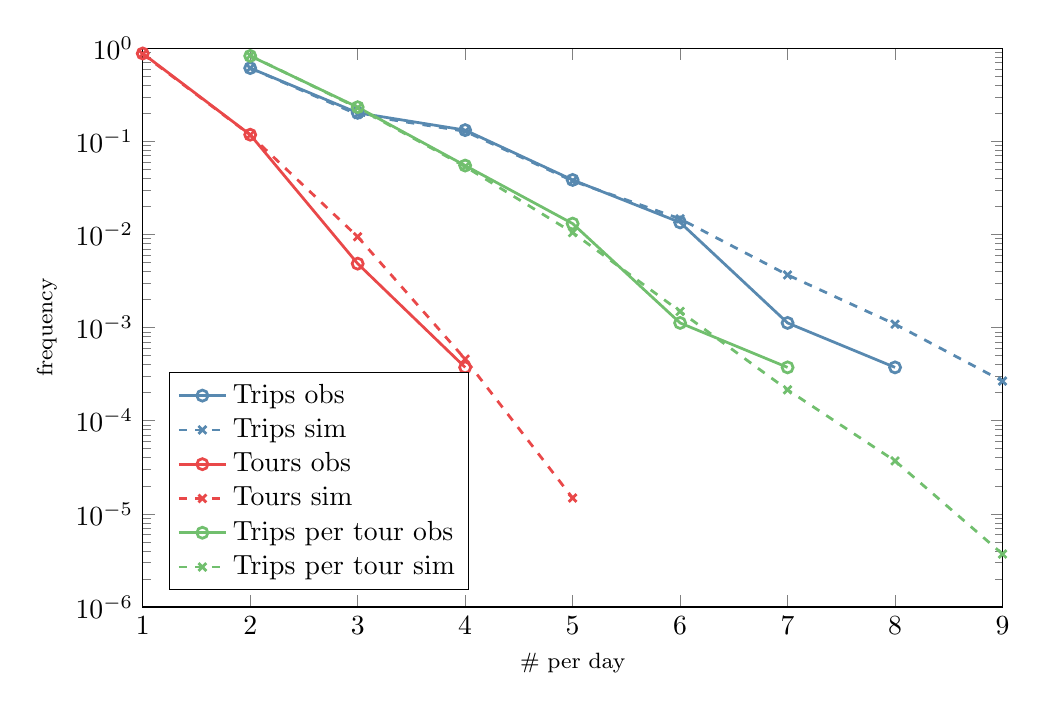
\begin{tikzpicture}

\begin{axis}[%
width=4.299in,
height=2.794in,
at={(0in,0in)},
scale only axis,
xmin=1,
xmax=9,
xlabel style={font=\footnotesize},
xlabel={\# per day},
ymode=log,
ymin=1e-06,
ymax=1,
yminorticks=true,
ylabel style={font=\footnotesize},
ylabel={frequency},
legend style={legend cell align=left, align=left},
legend pos = south west
]
\addplot [color=mycolor1, line width=1pt, mark=o, mark options={solid, mycolor1}]
  table[row sep=crcr]{%
2	0.6111\\
3	0.2021\\
4	0.1319\\
5	0.03848\\
6	0.01345\\
7	0.001121\\
8	0.0003736\\
};
\addlegendentry{Trips obs}

\addplot [color=mycolor1, dashed, line width=1pt, mark=x, mark options={solid, mycolor1}]
  table[row sep=crcr]{%
2	0.6105\\
3	0.1943\\
4	0.128\\
5	0.03754\\
6	0.0147\\
7	0.003676\\
8	0.001087\\
9	0.0002663\\
};
\addlegendentry{Trips sim}

\addplot [color=mycolor2, line width=1.0pt, mark=o, mark options={solid, mycolor2}]
  table[row sep=crcr]{%
1	0.8771\\
2	0.1177\\
3	0.004856\\
4	0.0003736\\
};
\addlegendentry{Tours obs}

\addplot [color=mycolor2, dashed, line width=1.0pt, mark=x, mark options={solid, mycolor2}]
  table[row sep=crcr]{%
1	0.8634\\
2	0.1168\\
3	0.009439\\
4	0.0004586\\
5	1.479e-05\\
};
\addlegendentry{Tours sim}

\addplot [color=mycolor3, line width=1.0pt, mark=o, mark options={solid, mycolor3}]
  table[row sep=crcr]{%
2	0.8252\\
3	0.2323\\
4	0.05491\\
5	0.01307\\
6	0.001121\\
7	0.0003736\\
};
\addlegendentry{Trips per tour obs}

\addplot [color=mycolor3, dashed, line width=1.0pt, mark=x, mark options={solid, mycolor3}]
  table[row sep=crcr]{%
2	0.8327\\
3	0.2287\\
4	0.05356\\
5	0.01047\\
6	0.001491\\
7	0.0002145\\
8	3.699e-05\\
9	3.699e-06\\
};
\addlegendentry{Trips per tour sim}

\end{axis}
\end{tikzpicture}%
	\caption{Distribution of number of trips, tours and trips per tour for simulated (dashed) and real data (solid). \label{fig:tours}}
\end{figure}

The length of trips by mode will mainly be determined by the utility of time and money for respectively mode and by network characteristics. This gives a good distribution of travel times, as can be seen in figure \ref{fig:triplength}. Since a large share of the trips are made to and from work, where the location is fixed and the trip is mandatory, the model is guaranteed to reproduce a large share of the trips well. However, the observed mode for the trip to work will only be the chosen mode in some of the simulated observations, and these restrictions will not give the distribution directly. 
%\begin{figure}[b!]
%\includegraphics[width=\textwidth]{fig/TripLength.png}
%\caption{Distribution of trip lengths of respectively mode for simulated (solid) and real data (dashed). \label{fig:triplength}}
%\end{figure}
\begin{figure}[b!]
%	% This file was created by matlab2tikz.
%
%The latest updates can be retrieved from
%  http://www.mathworks.com/matlabcentral/fileexchange/22022-matlab2tikz-matlab2tikz
%where you can also make suggestions and rate matlab2tikz.
%
\definecolor{mycolor1}{rgb}{0.34667,0.53600,0.69067}%
\definecolor{mycolor2}{rgb}{0.91529,0.28157,0.28784}%
\definecolor{mycolor3}{rgb}{0.44157,0.74902,0.43216}%
\definecolor{mycolor4}{rgb}{1.00000,0.59843,0.20000}%
%
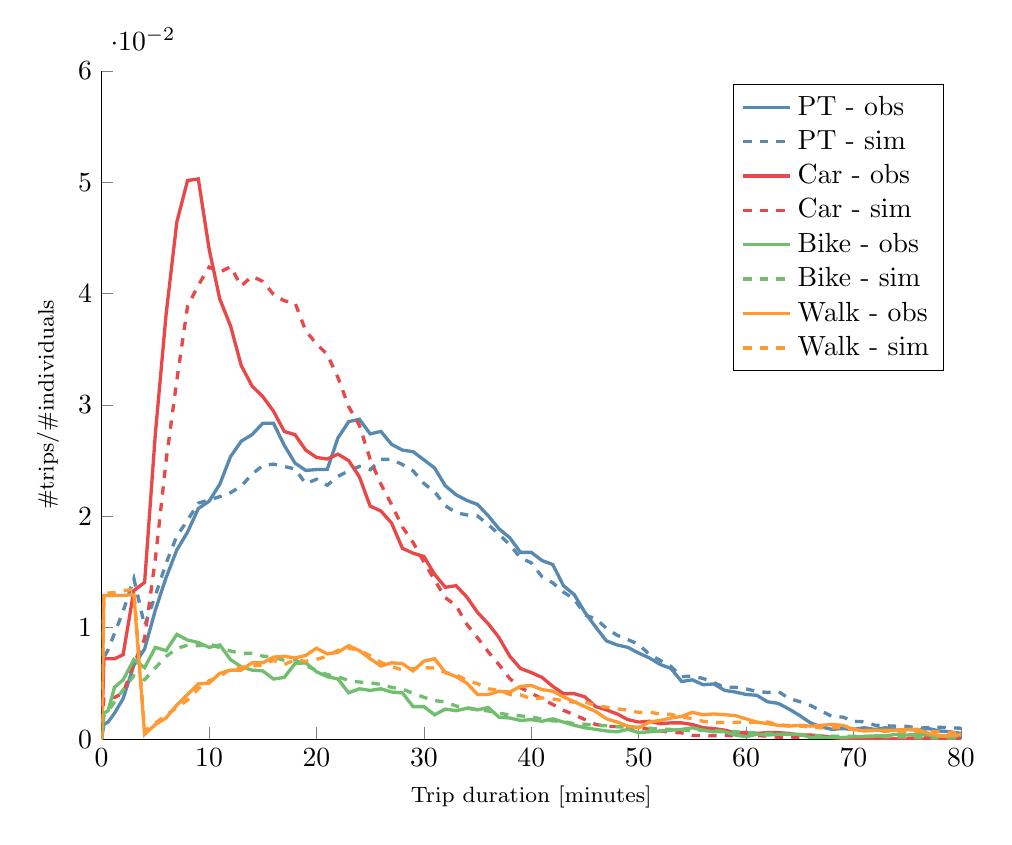
\begin{tikzpicture}

\begin{axis}[%
width=0.9\textwidth,
height=0.7\textwidth,
at={(0in,0in)},
scale only axis,
xmin=0,
xmax=80,
xlabel style={font=\footnotesize},
xlabel={Trip duration [minutes]},
ymin=0,
ymax=0.06,
ylabel style={font=\footnotesize},
ylabel={\#trips/\#individuals},
axis background/.style={fill=white},
axis x line*=bottom,
axis y line*=left,
legend style={legend cell align=left, align=left},
every axis plot/.append style = {very thick}
]
\addplot [color=mycolor1]
  table[row sep=crcr]{%
0	0\\
0.2	0.00131195335276968\\
0.6	0.00153061224489796\\
1.2	0.00233236151603499\\
2	0.00364431486880466\\
3	0.00663265306122449\\
4	0.00809037900874636\\
5	0.0115889212827988\\
6	0.0145043731778426\\
7	0.0169825072886297\\
8	0.0185860058309038\\
9	0.0206997084548105\\
10	0.0213556851311953\\
11	0.0228862973760933\\
12	0.0253644314868805\\
13	0.0267492711370262\\
14	0.027332361516035\\
15	0.0283527696793003\\
16	0.0283527696793003\\
17	0.0263848396501458\\
18	0.0247813411078717\\
19	0.0241253644314869\\
20	0.024198250728863\\
21	0.024198250728863\\
22	0.0270408163265306\\
23	0.0284985422740525\\
24	0.0287172011661808\\
25	0.0274052478134111\\
26	0.0276239067055394\\
27	0.0264577259475219\\
28	0.0259475218658892\\
29	0.025801749271137\\
30	0.0250728862973761\\
31	0.0243440233236152\\
32	0.0227405247813411\\
33	0.0219387755102041\\
34	0.0214285714285714\\
35	0.021064139941691\\
36	0.0200437317784257\\
37	0.0188775510204082\\
38	0.0180758017492711\\
39	0.0167638483965015\\
40	0.0167638483965015\\
41	0.0160349854227405\\
42	0.0156705539358601\\
43	0.0137755102040816\\
44	0.0129737609329446\\
45	0.0113702623906706\\
46	0.0100583090379009\\
47	0.00881924198250729\\
48	0.00845481049562682\\
49	0.00823615160349854\\
50	0.00772594752186589\\
51	0.00728862973760933\\
52	0.00670553935860058\\
53	0.00634110787172012\\
54	0.00517492711370262\\
55	0.00532069970845481\\
56	0.00488338192419825\\
57	0.00495626822157434\\
58	0.0043731778425656\\
59	0.00422740524781341\\
60	0.00400874635568513\\
61	0.00393586005830904\\
62	0.00335276967930029\\
63	0.00320699708454811\\
64	0.00269679300291545\\
65	0.00211370262390671\\
66	0.00145772594752187\\
67	0.0010932944606414\\
68	0.00087463556851312\\
69	0.000947521865889213\\
70	0.00087463556851312\\
71	0.00102040816326531\\
72	0.00087463556851312\\
73	0.00102040816326531\\
74	0.000801749271137026\\
75	0.00087463556851312\\
76	0.000801749271137026\\
77	0.000947521865889213\\
78	0.000728862973760933\\
79	0.00065597667638484\\
80	0.000510204081632653\\
81	0.00043731778425656\\
82	0.000291545189504373\\
83	0.00021865889212828\\
84	0.00021865889212828\\
85	7.28862973760933e-05\\
86	0\\
87	0\\
88	0\\
89	0.00021865889212828\\
90	0.000291545189504373\\
91	0.000291545189504373\\
92	0.000291545189504373\\
93	0.000291545189504373\\
94	7.28862973760933e-05\\
95	7.28862973760933e-05\\
96	7.28862973760933e-05\\
97	0.000145772594752187\\
98	0.000145772594752187\\
99	0.00021865889212828\\
100	0.000145772594752187\\
101	0.00021865889212828\\
102	0.000145772594752187\\
103	0.000145772594752187\\
104	7.28862973760933e-05\\
105	0.00021865889212828\\
106	0.00021865889212828\\
107	0.000291545189504373\\
108	0.000291545189504373\\
109	0.000291545189504373\\
110	0.000145772594752187\\
111	7.28862973760933e-05\\
112	7.28862973760933e-05\\
113	7.28862973760933e-05\\
114	7.28862973760933e-05\\
115	7.28862973760933e-05\\
116	7.28862973760933e-05\\
117	0.000291545189504373\\
};
\addlegendentry{PT - obs}

\addplot [color=mycolor1, dashed]
  table[row sep=crcr]{%
0	0\\
0.2	0.0073096452866861\\
0.6	0.00802028668610301\\
1.2	0.00950461613216715\\
2	0.0114696307094266\\
3	0.0144121720116618\\
4	0.0101766277939747\\
5	0.0128899416909621\\
6	0.0157780612244898\\
7	0.0182380952380952\\
8	0.0196468658892128\\
9	0.0211885325558795\\
10	0.0214658649173955\\
11	0.0217696793002915\\
12	0.0221224489795918\\
13	0.0227136783284742\\
14	0.0237849854227405\\
15	0.0245668124392614\\
16	0.0246864674441205\\
17	0.02447351797862\\
18	0.0242586248785228\\
19	0.0229341593780369\\
20	0.0233310252672498\\
21	0.0227930029154519\\
22	0.0235918367346939\\
23	0.0240817541302235\\
24	0.0244788629737609\\
25	0.0241831875607386\\
26	0.0251154033041788\\
27	0.025113824101069\\
28	0.0246537900874636\\
29	0.0240817541302235\\
30	0.0229539601554908\\
31	0.0222027453838678\\
32	0.0209515306122449\\
33	0.0203285957240039\\
34	0.0201310738581147\\
35	0.0200343780369291\\
36	0.0192509718172983\\
37	0.0183838678328474\\
38	0.0174444849368319\\
39	0.0162740524781341\\
40	0.0158284742468416\\
41	0.0145835762876579\\
42	0.0140313411078717\\
43	0.0131966715257532\\
44	0.0125810252672498\\
45	0.0111364188532556\\
46	0.0108101311953353\\
47	0.00994569970845481\\
48	0.00932009232264334\\
49	0.00893112244897959\\
50	0.00850911078717201\\
51	0.00759293002915452\\
52	0.00707689504373178\\
53	0.00653049076773566\\
54	0.00560835762876579\\
55	0.00565986394557823\\
56	0.00544144800777454\\
57	0.00508053935860058\\
58	0.00462585034013605\\
59	0.00465901360544218\\
60	0.00451737123420797\\
61	0.0042724732750243\\
62	0.00419059766763848\\
63	0.00427891156462585\\
64	0.00364965986394558\\
65	0.00336406705539359\\
66	0.00302113702623907\\
67	0.00254786200194363\\
68	0.0020205296404276\\
69	0.00197995626822157\\
70	0.00160119047619048\\
71	0.0015597667638484\\
72	0.00125291545189504\\
73	0.00119910106899903\\
74	0.00115974246841594\\
75	0.00114249271137026\\
76	0.000976190476190476\\
77	0.00104215257531584\\
78	0.00106584062196307\\
79	0.0010074101068999\\
80	0.00098153547133139\\
81	0.000959548104956268\\
82	0.000896137026239067\\
83	0.000712342079689018\\
84	0.000637998056365403\\
85	0.000524781341107872\\
86	0.000461491739552964\\
87	0.00038022351797862\\
88	0.000314261418853256\\
89	0.000260568513119533\\
90	0.000145408163265306\\
91	8.43051506316813e-05\\
92	0.000122084548104956\\
93	0.000125728862973761\\
94	9.99757045675413e-05\\
95	0.000124392614188533\\
96	0.000121234207968902\\
97	0.000137147716229349\\
98	0.000123177842565598\\
99	0.000157798833819242\\
100	0.000114795918367347\\
101	0.000176263362487852\\
102	0.000164601554907677\\
103	0.000162900874635569\\
104	0.000125242954324587\\
105	0.000284378036929057\\
106	0.000220724003887269\\
107	0.000193391642371234\\
108	0.000193999028182702\\
109	0.000193634596695821\\
110	3.31632653061225e-05\\
111	3.15840621963071e-05\\
112	2.28377065111759e-05\\
113	3.49854227405248e-05\\
114	3.60787172011662e-05\\
115	4.93197278911565e-05\\
116	4.95626822157434e-05\\
117	0.000177478134110787\\
};
\addlegendentry{PT - sim}

\addplot [color=mycolor2]
  table[row sep=crcr]{%
0	0\\
0.2	0.00721574344023324\\
0.6	0.00721574344023324\\
1.2	0.00721574344023324\\
2	0.0075801749271137\\
3	0.0133381924198251\\
4	0.014067055393586\\
5	0.0274052478134111\\
6	0.0381195335276968\\
7	0.0464285714285714\\
8	0.0501457725947522\\
9	0.0502915451895044\\
10	0.0440233236151603\\
11	0.0395043731778426\\
12	0.0370991253644315\\
13	0.0335276967930029\\
14	0.0317055393586006\\
15	0.0307580174927114\\
16	0.0294460641399417\\
17	0.0276239067055394\\
18	0.027332361516035\\
19	0.0259475218658892\\
20	0.0252915451895044\\
21	0.0251457725947522\\
22	0.0255830903790087\\
23	0.025\\
24	0.0235422740524781\\
25	0.0209183673469388\\
26	0.0204810495626822\\
27	0.0193877551020408\\
28	0.0171282798833819\\
29	0.0166909620991254\\
30	0.016399416909621\\
31	0.0147959183673469\\
32	0.0136297376093294\\
33	0.0137755102040816\\
34	0.0127551020408163\\
35	0.0113702623906706\\
36	0.0103498542274052\\
37	0.00911078717201166\\
38	0.00743440233236152\\
39	0.00634110787172012\\
40	0.00597667638483965\\
41	0.00553935860058309\\
42	0.00473760932944606\\
43	0.00408163265306122\\
44	0.00408163265306122\\
45	0.00379008746355685\\
46	0.00291545189504373\\
47	0.00262390670553936\\
48	0.00225947521865889\\
49	0.00174927113702624\\
50	0.00153061224489796\\
51	0.00160349854227405\\
52	0.00138483965014577\\
53	0.00145772594752187\\
54	0.00145772594752187\\
55	0.00131195335276968\\
56	0.00102040816326531\\
57	0.000947521865889213\\
58	0.000801749271137026\\
59	0.000583090379008746\\
60	0.000583090379008746\\
61	0.000510204081632653\\
62	0.000583090379008746\\
63	0.000583090379008746\\
64	0.000510204081632653\\
65	0.000364431486880466\\
66	0.000364431486880466\\
67	0.000291545189504373\\
68	0.000145772594752187\\
69	7.28862973760933e-05\\
70	7.28862973760933e-05\\
71	0\\
72	0\\
73	0\\
74	0\\
75	0\\
76	0\\
77	0\\
78	0\\
79	0\\
80	0\\
81	0\\
82	0\\
83	7.28862973760933e-05\\
84	7.28862973760933e-05\\
85	0.000145772594752187\\
86	0.000145772594752187\\
87	0.000145772594752187\\
88	7.28862973760933e-05\\
89	7.28862973760933e-05\\
90	0\\
91	0\\
92	0\\
93	0\\
94	0\\
95	0\\
96	0\\
97	0\\
98	0\\
99	0\\
100	0\\
101	0\\
102	0\\
103	0\\
104	0\\
105	0\\
106	0\\
107	7.28862973760933e-05\\
108	7.28862973760933e-05\\
109	7.28862973760933e-05\\
110	0.00021865889212828\\
111	0.00021865889212828\\
112	0.000145772594752187\\
113	0.000145772594752187\\
114	0.00021865889212828\\
115	7.28862973760933e-05\\
116	7.28862973760933e-05\\
117	7.28862973760933e-05\\
};
\addlegendentry{Car - obs}

\addplot [color=mycolor2, dashed]
  table[row sep=crcr]{%
0	0\\
0.2	0.00373955296404276\\
0.6	0.00373955296404276\\
1.2	0.00373955296404276\\
2	0.00415063168124393\\
3	0.00675898931000972\\
4	0.0090336491739553\\
5	0.0161873177842566\\
6	0.0249821428571429\\
7	0.0322192662779397\\
8	0.0388583576287658\\
9	0.0407502429543246\\
10	0.0423804664723032\\
11	0.0419165451895044\\
12	0.042405612244898\\
13	0.0406897473275024\\
14	0.0415481049562682\\
15	0.0410945092322643\\
16	0.0399249271137026\\
17	0.0393479105928086\\
18	0.0391806365403304\\
19	0.0366644800777454\\
20	0.0354769193391642\\
21	0.0345343780369291\\
22	0.0324653790087464\\
23	0.0298442662779397\\
24	0.0281673955296404\\
25	0.0251163751214772\\
26	0.0228910349854227\\
27	0.0210504130223518\\
28	0.019046768707483\\
29	0.0176540330417881\\
30	0.0158991739552964\\
31	0.0142706511175899\\
32	0.012700315840622\\
33	0.0119934402332362\\
34	0.0103111030126336\\
35	0.00909839650145773\\
36	0.00782543731778426\\
37	0.00667954324586978\\
38	0.0054365889212828\\
39	0.00462062682215743\\
40	0.00411880466472303\\
41	0.00362487852283771\\
42	0.00311115160349854\\
43	0.00258491253644315\\
44	0.00218974732750243\\
45	0.00175157920310982\\
46	0.00131584062196307\\
47	0.0011435860058309\\
48	0.00112585034013605\\
49	0.000939868804664723\\
50	0.00100413022351798\\
51	0.000895165208940719\\
52	0.000717930029154519\\
53	0.000621355685131195\\
54	0.000560009718172983\\
55	0.000335034013605442\\
56	0.000311224489795918\\
57	0.000295553935860058\\
58	0.000328960155490768\\
59	0.000295189504373178\\
60	0.000341472303206997\\
61	0.000315597667638484\\
62	0.000270165208940719\\
63	0.000160957240038873\\
64	0.00019290573372206\\
65	0.000162536443148688\\
66	0.000225340136054422\\
67	0.000217444120505345\\
68	0.000146622934888241\\
69	0.000111516034985423\\
70	7.27648202137998e-05\\
71	8.26044703595724e-06\\
72	8.86783284742468e-06\\
73	7.41010689990282e-06\\
74	7.16715257531584e-06\\
75	7.1064139941691e-05\\
76	0.000122691933916424\\
77	0.00012257045675413\\
78	0.000123299319727891\\
79	0.000124271137026239\\
80	6.07385811467444e-05\\
81	9.11078717201166e-06\\
82	7.28862973760933e-06\\
83	1.67638483965015e-05\\
84	1.56705539358601e-05\\
85	3.09766763848397e-05\\
86	2.93974732750243e-05\\
87	2.95189504373178e-05\\
88	1.84645286686103e-05\\
89	1.82215743440233e-05\\
90	2.30806608357629e-06\\
91	3.2798833819242e-06\\
92	3.15840621963071e-06\\
93	3.40136054421769e-06\\
94	3.40136054421769e-06\\
95	3.52283770651118e-06\\
96	2.55102040816327e-06\\
97	2.67249757045675e-06\\
98	2.91545189504373e-06\\
99	2.79397473275024e-06\\
100	2.55102040816327e-06\\
101	2.55102040816327e-06\\
102	2.30806608357629e-06\\
103	2.1865889212828e-06\\
104	2.55102040816327e-06\\
105	2.55102040816327e-06\\
106	2.1865889212828e-06\\
107	7.25218658892128e-05\\
108	7.22789115646259e-05\\
109	7.19144800777454e-05\\
110	7.17930029154519e-05\\
111	7.17930029154519e-05\\
112	8.50340136054422e-07\\
113	6.07385811467444e-07\\
114	4.62827988338192e-05\\
115	4.62827988338192e-05\\
116	4.65257531584062e-05\\
117	4.66472303206997e-05\\
};
\addlegendentry{Car - sim}

\addplot [color=mycolor3]
  table[row sep=crcr]{%
0	0\\
0.2	0.00233236151603499\\
0.6	0.00255102040816327\\
1.2	0.00466472303206997\\
2	0.00532069970845481\\
3	0.00714285714285714\\
4	0.00641399416909621\\
5	0.00823615160349854\\
6	0.00794460641399417\\
7	0.00940233236151604\\
8	0.00889212827988338\\
9	0.0086734693877551\\
10	0.00823615160349854\\
11	0.00845481049562682\\
12	0.00714285714285714\\
13	0.0064868804664723\\
14	0.00619533527696793\\
15	0.00612244897959184\\
16	0.0053935860058309\\
17	0.00553935860058309\\
18	0.00677842565597668\\
19	0.00685131195335277\\
20	0.00604956268221574\\
21	0.00561224489795918\\
22	0.0053935860058309\\
23	0.00415451895043732\\
24	0.00451895043731778\\
25	0.0043731778425656\\
26	0.00451895043731778\\
27	0.00422740524781341\\
28	0.00415451895043732\\
29	0.00291545189504373\\
30	0.00291545189504373\\
31	0.0021865889212828\\
32	0.00269679300291545\\
33	0.00255102040816327\\
34	0.00276967930029155\\
35	0.00262390670553936\\
36	0.00284256559766764\\
37	0.00196793002915452\\
38	0.00189504373177843\\
39	0.00167638483965015\\
40	0.00174927113702624\\
41	0.00160349854227405\\
42	0.00182215743440233\\
43	0.00153061224489796\\
44	0.00123906705539359\\
45	0.00102040816326531\\
46	0.00087463556851312\\
47	0.000728862973760933\\
48	0.00065597667638484\\
49	0.00087463556851312\\
50	0.000583090379008746\\
51	0.00065597667638484\\
52	0.000728862973760933\\
53	0.000801749271137026\\
54	0.00087463556851312\\
55	0.00102040816326531\\
56	0.000801749271137026\\
57	0.00065597667638484\\
58	0.00065597667638484\\
59	0.000364431486880466\\
60	0.00021865889212828\\
61	0.00043731778425656\\
62	0.000364431486880466\\
63	0.00043731778425656\\
64	0.00043731778425656\\
65	0.00043731778425656\\
66	0.000145772594752187\\
67	0.000145772594752187\\
68	0.000145772594752187\\
69	0.000145772594752187\\
70	0.00021865889212828\\
71	0.00021865889212828\\
72	0.000291545189504373\\
73	0.000291545189504373\\
74	0.00043731778425656\\
75	0.000364431486880466\\
76	0.00043731778425656\\
77	0.000364431486880466\\
78	0.000291545189504373\\
79	0.00021865889212828\\
80	0.000364431486880466\\
81	0.000364431486880466\\
82	0.00043731778425656\\
83	0.00043731778425656\\
84	0.00043731778425656\\
85	0.000291545189504373\\
86	0.00021865889212828\\
87	0.000145772594752187\\
88	7.28862973760933e-05\\
89	0\\
90	0\\
91	7.28862973760933e-05\\
92	7.28862973760933e-05\\
93	7.28862973760933e-05\\
94	7.28862973760933e-05\\
95	0.000145772594752187\\
96	0.000145772594752187\\
97	0.000145772594752187\\
98	0.000145772594752187\\
99	0.000145772594752187\\
100	7.28862973760933e-05\\
101	0.000145772594752187\\
102	0.000145772594752187\\
103	0.000145772594752187\\
104	0.000145772594752187\\
105	0.000145772594752187\\
106	0\\
107	0\\
108	0\\
109	0\\
110	0\\
111	0\\
112	0\\
113	0\\
114	7.28862973760933e-05\\
115	7.28862973760933e-05\\
116	0.000145772594752187\\
117	0.000291545189504373\\
};
\addlegendentry{Bike - obs}

\addplot [color=mycolor3, dashed]
  table[row sep=crcr]{%
0	0\\
0.2	0.00207956754130224\\
0.6	0.00248226433430515\\
1.2	0.00336601068999028\\
2	0.00443221574344023\\
3	0.00568500971817298\\
4	0.00532774538386783\\
5	0.00639504373177842\\
6	0.00741715257531584\\
7	0.00814224975704568\\
8	0.00843598153547133\\
9	0.00837779397473275\\
10	0.00856499028182702\\
11	0.00820347424684159\\
12	0.00791569484936832\\
13	0.00769484936831876\\
14	0.00770833333333333\\
15	0.00745201652089407\\
16	0.00735993683187561\\
17	0.00706972789115646\\
18	0.0071082361516035\\
19	0.00661321671525753\\
20	0.00616375121477162\\
21	0.00578765792031098\\
22	0.00560519922254616\\
23	0.0052463556851312\\
24	0.00512390670553936\\
25	0.00505478620019436\\
26	0.00491277939747327\\
27	0.00464067055393586\\
28	0.00450218658892128\\
29	0.00410131195335277\\
30	0.00375874635568513\\
31	0.00345505344995141\\
32	0.00334900388726919\\
33	0.00297120991253644\\
34	0.00283442662779397\\
35	0.00265415451895044\\
36	0.00252223032069971\\
37	0.00232847424684159\\
38	0.00216885325558795\\
39	0.00208466958211856\\
40	0.00199829931972789\\
41	0.00179968415937804\\
42	0.00163751214771623\\
43	0.00157932458697765\\
44	0.00138168124392614\\
45	0.00133345481049563\\
46	0.0012593537414966\\
47	0.00120177356656948\\
48	0.0011064139941691\\
49	0.00107810981535471\\
50	0.00105988824101069\\
51	0.000980320699708455\\
52	0.000900267249757046\\
53	0.000871355685131195\\
54	0.0008283527696793\\
55	0.000765427599611273\\
56	0.000780369290573372\\
57	0.000755952380952381\\
58	0.000725704567541302\\
59	0.000665087463556851\\
60	0.00060653547133139\\
61	0.000552478134110787\\
62	0.000503158406219631\\
63	0.000468901846452867\\
64	0.00040913508260447\\
65	0.00039067055393586\\
66	0.000331875607385811\\
67	0.000292031098153547\\
68	0.000266156462585034\\
69	0.00026044703595724\\
70	0.000246720116618076\\
71	0.000253279883381924\\
72	0.000247327502429543\\
73	0.000223275024295432\\
74	0.000205903790087464\\
75	0.000170918367346939\\
76	0.000139941690962099\\
77	0.000119290573372206\\
78	0.000105442176870748\\
79	0.000100826044703596\\
80	0.000105442176870748\\
81	9.96112730806608e-05\\
82	9.29300291545189e-05\\
83	9.03790087463557e-05\\
84	8.50340136054422e-05\\
85	7.39795918367347e-05\\
86	7.17930029154519e-05\\
87	6.81486880466472e-05\\
88	5.988824101069e-05\\
89	5.64868804664723e-05\\
90	5.24781341107872e-05\\
91	4.49465500485909e-05\\
92	4.3245869776482e-05\\
93	4.08163265306122e-05\\
94	3.42565597667639e-05\\
95	3.13411078717201e-05\\
96	2.90330417881438e-05\\
97	2.86686103012634e-05\\
98	3.04907677356657e-05\\
99	3.02478134110787e-05\\
100	2.80612244897959e-05\\
101	2.59961127308066e-05\\
102	2.34450923226433e-05\\
103	1.78571428571429e-05\\
104	1.49416909620991e-05\\
105	1.57920310981535e-05\\
106	1.50631681243926e-05\\
107	1.22691933916424e-05\\
108	1.16618075801749e-05\\
109	9.83965014577259e-06\\
110	8.38192419825073e-06\\
111	7.04567541302235e-06\\
112	6.80272108843537e-06\\
113	5.95238095238095e-06\\
114	5.83090379008746e-06\\
115	6.31681243926142e-06\\
116	4.73760932944606e-06\\
117	2.52672497570457e-05\\
};
\addlegendentry{Bike - sim}

\addplot [color=mycolor4]
  table[row sep=crcr]{%
0	0\\
0.2	0.0129008746355685\\
0.6	0.0129008746355685\\
1.2	0.0129008746355685\\
2	0.0129008746355685\\
3	0.0129737609329446\\
4	0.00043731778425656\\
5	0.00131195335276968\\
6	0.00189504373177843\\
7	0.00306122448979592\\
8	0.00400874635568513\\
9	0.00495626822157434\\
10	0.00502915451895044\\
11	0.00590379008746356\\
12	0.00619533527696793\\
13	0.00619533527696793\\
14	0.00685131195335277\\
15	0.00685131195335277\\
16	0.00736151603498542\\
17	0.00743440233236152\\
18	0.00728862973760933\\
19	0.00750728862973761\\
20	0.00816326530612245\\
21	0.0076530612244898\\
22	0.00779883381924198\\
23	0.00838192419825073\\
24	0.00794460641399417\\
25	0.00721574344023324\\
26	0.0065597667638484\\
27	0.00685131195335277\\
28	0.00677842565597668\\
29	0.00612244897959184\\
30	0.00699708454810496\\
31	0.00721574344023324\\
32	0.00597667638483965\\
33	0.00561224489795918\\
34	0.00502915451895044\\
35	0.00400874635568513\\
36	0.00400874635568513\\
37	0.00430029154518951\\
38	0.00422740524781341\\
39	0.00473760932944606\\
40	0.00481049562682216\\
41	0.00444606413994169\\
42	0.00430029154518951\\
43	0.00379008746355685\\
44	0.00335276967930029\\
45	0.00291545189504373\\
46	0.00247813411078717\\
47	0.00182215743440233\\
48	0.00153061224489796\\
49	0.00116618075801749\\
50	0.00102040816326531\\
51	0.00153061224489796\\
52	0.00167638483965015\\
53	0.00189504373177843\\
54	0.00204081632653061\\
55	0.00240524781341108\\
56	0.0021865889212828\\
57	0.00225947521865889\\
58	0.0021865889212828\\
59	0.00211370262390671\\
60	0.00182215743440233\\
61	0.00153061224489796\\
62	0.00138483965014577\\
63	0.00123906705539359\\
64	0.00116618075801749\\
65	0.00123906705539359\\
66	0.00116618075801749\\
67	0.00123906705539359\\
68	0.00131195335276968\\
69	0.00123906705539359\\
70	0.00087463556851312\\
71	0.000728862973760933\\
72	0.000801749271137026\\
73	0.000801749271137026\\
74	0.000801749271137026\\
75	0.00087463556851312\\
76	0.00087463556851312\\
77	0.000510204081632653\\
78	0.000291545189504373\\
79	0.000291545189504373\\
80	0.00043731778425656\\
81	0.000510204081632653\\
82	0.00043731778425656\\
83	0.000510204081632653\\
84	0.000364431486880466\\
85	0.000145772594752187\\
86	0.000145772594752187\\
87	0.000291545189504373\\
88	0.00021865889212828\\
89	0.00021865889212828\\
90	0.000364431486880466\\
91	0.000291545189504373\\
92	0.000145772594752187\\
93	0.000291545189504373\\
94	0.000291545189504373\\
95	0.000145772594752187\\
96	0.000145772594752187\\
97	0.000145772594752187\\
98	0\\
99	7.28862973760933e-05\\
100	7.28862973760933e-05\\
101	0.000145772594752187\\
102	0.000145772594752187\\
103	0.000145772594752187\\
104	7.28862973760933e-05\\
105	7.28862973760933e-05\\
106	0\\
107	7.28862973760933e-05\\
108	7.28862973760933e-05\\
109	0.000145772594752187\\
110	0.000145772594752187\\
111	0.00021865889212828\\
112	0.000145772594752187\\
113	0.00021865889212828\\
114	0.00021865889212828\\
115	0.00021865889212828\\
116	0.00021865889212828\\
117	0.00043731778425656\\
};
\addlegendentry{Walk - obs}

\addplot [color=mycolor4, dashed]
  table[row sep=crcr]{%
0	0\\
0.2	0.0130970602526725\\
0.6	0.0131183187560739\\
1.2	0.0131437074829932\\
2	0.0132995626822157\\
3	0.0134716958211856\\
4	0.000732871720116618\\
5	0.00143488824101069\\
6	0.00216836734693878\\
7	0.00282240038872692\\
8	0.00351882896015549\\
9	0.00453194849368319\\
10	0.00524611273080661\\
11	0.00560532069970845\\
12	0.00630660835762877\\
13	0.00642857142857143\\
14	0.00658053935860058\\
15	0.00663216715257532\\
16	0.00708199708454811\\
17	0.00669557823129252\\
18	0.00711831875607386\\
19	0.00698821671525753\\
20	0.00715585519922255\\
21	0.00744071914480078\\
22	0.0079758260447036\\
23	0.00816010689990282\\
24	0.00799125364431487\\
25	0.00747776967930029\\
26	0.00687840136054422\\
27	0.00652162293488824\\
28	0.00620262390670554\\
29	0.00631778425655977\\
30	0.00641253644314869\\
31	0.00637815840621963\\
32	0.00597509718172983\\
33	0.00578510689990282\\
34	0.00527174441205053\\
35	0.00497971331389699\\
36	0.00451530612244898\\
37	0.00439698736637512\\
38	0.00400036443148688\\
39	0.00397120991253644\\
40	0.00362159863945578\\
41	0.00370201652089407\\
42	0.00360495626822157\\
43	0.00344448493683188\\
44	0.00331073858114674\\
45	0.00334463070942663\\
46	0.00299854227405248\\
47	0.00286771137026239\\
48	0.00272278911564626\\
49	0.00259961127308066\\
50	0.00239249271137026\\
51	0.00242674927113703\\
52	0.00224562682215743\\
53	0.00222303206997085\\
54	0.00197096695821186\\
55	0.00184851797862002\\
56	0.00159657434402332\\
57	0.0014608843537415\\
58	0.00149744897959184\\
59	0.0015\\
60	0.00151797862001944\\
61	0.00150801749271137\\
62	0.00153838678328474\\
63	0.00129907677356657\\
64	0.00121404275996113\\
65	0.00117334791059281\\
66	0.00109183673469388\\
67	0.00101214771622935\\
68	0.00103705053449951\\
69	0.00100983965014577\\
70	0.000856778425655977\\
71	0.000812074829931973\\
72	0.000747934888241011\\
73	0.000707240038872692\\
74	0.000706146744412051\\
75	0.000678206997084548\\
76	0.000715621963070943\\
77	0.000711856171039844\\
78	0.000654033041788144\\
79	0.000579567541302235\\
80	0.000580539358600583\\
81	0.000470359572400389\\
82	0.000430636540330418\\
83	0.000436588921282799\\
84	0.000416545189504373\\
85	0.000381559766763848\\
86	0.000393221574344023\\
87	0.000379494655004859\\
88	0.000348760932944606\\
89	0.000315233236151603\\
90	0.000316933916423712\\
91	0.000294460641399417\\
92	0.000262512147716229\\
93	0.000251700680272109\\
94	0.000250121477162293\\
95	0.000239431486880466\\
96	0.000236030126336249\\
97	0.000239067055393586\\
98	0.000221817298347911\\
99	0.000207968901846453\\
100	0.00017930029154519\\
101	0.000171282798833819\\
102	0.00016435860058309\\
103	0.000157191448007775\\
104	0.000158041788143829\\
105	0.00016120019436346\\
106	0.000143586005830904\\
107	0.000143586005830904\\
108	0.00013301749271137\\
109	0.00011698250728863\\
110	0.000110422740524781\\
111	0.000109936831875607\\
112	9.7667638483965e-05\\
113	9.63313896987366e-05\\
114	9.17152575315841e-05\\
115	9.05004859086492e-05\\
116	8.33333333333333e-05\\
117	0.000316083576287658\\
};
\addlegendentry{Walk - sim}

\end{axis}
\end{tikzpicture}%
	\caption{Distribution of trip lengths of respectively mode for observed choices (solid) and simulated (dashed). The plot has been obtained by first constructing a histogram with bin-size of one minute, and then average each time step over the closest 5 minutes. \label{fig:triplength}}
\end{figure}
 
% To do- also plot activity duration



The ``same zone'' dummy parameter \param{same zone} for walk is negative, which seems contra-intuitive as one would expect walk to be the preferred mode of transport for shorter distances. From figure \ref{fig:triplength} it is clear that for same-zone trips (trips with zero travel time) walk is still the preferred mode of transport. The reason for this is that the mode specific constant $C_{\text{walk}}$ is the largest of the constants, even after adding $\delta_{\text{same zone}}$, and when the travel time is small it will therefore have the highest utility.

The parameters for travel time are almost the same for car, walk and bike but significantly smaller for PT. Since the travel time is longer for bike and walk, they will be less common for longer trips. PT has the smallest time coefficient and trips with longer travel time are therefore more common with public transport. The lower speed of bike and walk in comparison with the motorized modes will make them less common for longer trips, as can be seen in figure \ref{fig:triplength}. The lower alternative specific constants, and the fact that more locations will become available with the same travel time with PT and car also make bike and walk less common.



